	\documentclass[10pt,oneside]{CBFT_book}
	
	% Paquetes que cargan
	
	\usepackage{standalone}
	\usepackage{amssymb}
	\usepackage{amsmath}
	\usepackage{graphicx}
	\usepackage{libertine}
	\usepackage[bold-style=TeX]{unicode-math}
	\usepackage{lipsum}

	\usepackage[numbers]{natbib}
	\setcitestyle{square}

	\usepackage{polyglossia}
	\setdefaultlanguage{spanish}
	
	\usepackage{CBFT.estilo} % Cargo la hoja de estilo
	
	\title{CURSO BÁSICO DE FÍSICA TEÓRICA}
	\subtitle{Volumen 4: Física Teórica 3 [Mecánica Estadística]}
	\author{E.F. Lavia}
	\date{\today}
	\version{versión 0.1}

	%###########################################################################
	%		DOCUMENTO 
	%###########################################################################
	
	\begin{document}
	\maketitle	
	
%	\pagenumbering{roman}
	\thispagestyle{empty}
	
	\tableofcontents
	
	\thispagestyle{empty}
	
	
% 	\listoffigures
	
% 	\listoftables

% 	\include{chaps/cft_prefacio}

	\clearpage

	%###########################################################################
	%		CAPITULOS DEL CURSO
	%###########################################################################
	
	\pagenumbering{arabic}
	
		\documentclass[10pt,oneside]{CBFT_book}
	% Algunos paquetes
	\usepackage{amssymb}
	\usepackage{amsmath}
	\usepackage{graphicx}
	\usepackage{libertine}
	\usepackage[bold-style=TeX]{unicode-math}
	\usepackage{lipsum}

	\usepackage{natbib}
	\setcitestyle{square}

	\usepackage{polyglossia}
	\setdefaultlanguage{spanish}
	



	\usepackage{CBFT.estilo} % Cargo la hoja de estilo

	% Tipografías
	% \setromanfont[Mapping=tex-text]{Linux Libertine O}
	% \setsansfont[Mapping=tex-text]{DejaVu Sans}
	% \setmonofont[Mapping=tex-text]{DejaVu Sans Mono}

	%===================================================================
	%	DOCUMENTO PROPIAMENTE DICHO
	%===================================================================

\begin{document}

% =================================================================================================
\chapter{Básicos de termodinámica}
% =================================================================================================


% =================================================================================================
\section{Energía y entropía}
% =================================================================================================

Una de las formulaciones de la 2da ley es definir la entropía. Surge de:
\[
	\frac{Q_1}{Q_2} = -\frac{T_1}{T_2} \qquad \Rightarrow \frac{Q_1}{Q_2} + \frac{T_1}{T_2} = 0 \;
	\text{reversible}
\]
\[
	\int \frac{dQ}{T} \leq 0 \qquad \text{desigualdad de Clausius}
\] 
Proceso reversible en un sistema aislado
\[
	S_{A\to B} = \int_A^B dS = 0
\]
pues 
\[
	dS =\frac{dU}{T} - \frac{p}{V}dV + \frac{\mu}{T}dN = 0
\]
pero en procesos irreversibles la variación de $S$ es cota superior:
\notamargen{La existencia de $S$ es independiente de su cálculo}
\[
	\int_A^B \frac{dQ}{T} < \int_A^B dS = S_{A\to B}.
\]

Luego, para un sistema aislado, en un proceso irreversible 
\[
	dS_I = 0 \qquad \Rightarrow \qquad \frac{dQ_I}{T} = 0
\]
y entonces
\[
	0 < \int_A^B  dS =  S_{A\to B}
\]

La entropía solo aumenta. Podría calcular $S_{A\to B}$ con un proceso reversible de $A\to B$ pero ahí 
ya tengo que intervenir sobre el sistema (no hay procesos espontáneos --en un sistema aislado-- reversibles).

En reversibles
\[
	dU = TdS - pdV + \mu dN
\]
mientras que en irreversibles
\[
	dU = ddQ_I - pdV +\mu dN, \quad \text{pero} \quad dQ_I < TdS 
\]
y entonces
\[
	dU < TdS - pdV + \mu dN
\]
% \begin{figure}[htb]
% 	\begin{center}
% 	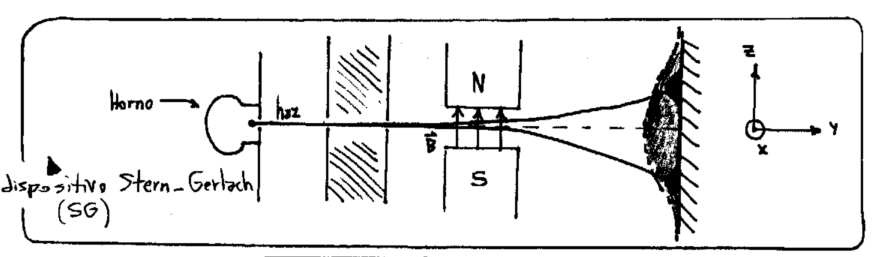
\includegraphics[width=0.8\textwidth]{images/teo2_1.pdf}	 
% 	\end{center}
% 	\caption{}
% \end{figure} 
Si $S$ es homogénea, se tiene
\[
	S = S(\lambda U, \lambda X, \{\lambda N_i\}) = \lambda S( U, X, \{ N_i\})
\]
y además si \notamargen{En un sistema $PVT$ $Y=-p$.}
\[
	TdS = dU - YdX - \mu_i dN_i
\]
\[
	\dtot{S}{\lambda} = S = \dpar{S}{\lambda U}\dtot{\lambda U}{\lambda} +
	\dpar{S}{\lambda X}\dtot{\lambda X}{\lambda} +
	\dpar{S}{\lambda N_i}\dtot{\lambda N_i}{\lambda}
\]
\[
	S = \dpar{S}{\lambda U} U + \dpar{S}{\lambda X} X + \dpar{S}{\lambda N_i} N_i
\]
\[
	\dpar{}{\lambda U}\left[ S(\lambda U)\right] = 
	\dpar{}{\lambda U}\left[ \lambda S( U)\right] = \dpar{S}{U} = \frac{1}{T}
\]
y procediendo del mismo modo con $Y,\mu$
\[
	S = \frac{1}{T} U + \frac{-Y}{T} X + \frac{-\mu_i}{T} N_i
\]
y arribamos a la ecuación fundamental
\[
	TS = U - YX - \mu_i N_i 
\]
o bien
\[
	U = TS + YX + \sum_i \mu_i N_i
\]

La primera ley (en sistemas reversibles) era 
\[
	dU = TdS + YdX + \sum_i \mu_i dN_i
\]
y a $S,V,N$ constantes 
\[
	dU^R = 0 \qquad dU^I \leq 0
\]
la mínima $U$ es equilibrio.
Si existe trabajo que no es de volumen resulta 
\[
	dU < -dW_\text{libre}
\]
\[
	\frac{dQ}{dT} = \frac{dU}{T} + \frac{p}{T}dV - \frac{\mu}{T}dN = \frac{dQ}{dT} \leq dS
\]

Si el sistema está aislado será
\[
	0 \leq dS \quad \text{condición de equilibrio}
\]
alcanzando el máximo ya no puede disminuir la entropía.


% =================================================================================================
\section{Transformadas de Legendre de las funciones termodinámicas}
% =================================================================================================

\[
	f(x,y,z) \qquad \text{con pendientes} \quad \dpar{f}{x},\dpar{f}{y},\dpar{f}{z}
\]
entonces 
\[
	\varphi(f_x,y,z) = f(x,y,z) - \left. x \dpar{f(x,y,z)}{x}\right|_{y,z}
\]
es la transformada de Legendre respecto de $x$, mientras que 
\[
	\varphi(f_x,f_y,z) = f(x,y,z) - x \dpar{f}{x} - y \dpar{f}{y}
\]
es la transformada de Legendre respecto de $y$.

La transformada de Legendre transforma una función homogénea en otra función homogénea, mantiene el
carácter de función de estado.
\[
	d\varphi(f_x,y,z) = df - dx \dpar{f}{x} - x d\left( \dpar{f}{y} \right)
\]

Para el caso de la energía
\[
	U=U(S,V,N) \qquad \qquad dU = TdS - pdV + \mu dN
\]
y entonces
\[
	A = U - \left. S\dpar{U}{S}\right|_{V,N} = U - ST \Rightarrow A=A(T,V,N)
\]
% \[
% 	\left( \frac{1}{\sqrt{2}} \Bra{x} + \frac{1}{\sqrt{2}} \Bra{y}  \right)
% 	\left( \Ket{x} \right)= \frac{1}{\sqrt{2}}
% \]
% 
% \subsection{Propiedades}
% 
% \begin{enumerate}
%  \item $\Braket{\beta|\alpha} = \Braket{\beta|\alpha}^*$ \text{luego} $ \Braket{\alpha|\alpha} \; \in \mathbb{R}$
%  \item $\Braket{\alpha|\alpha} \geq 0$ \text{métrica definida positiva}
%  \item $\Braket{\alpha|\beta} = \Braket{\beta|\alpha} = 0 \Leftrightarrow \Ket{\alpha} \perp \Ket{\beta}$
%  \item $\Braket{\tilde{\alpha}|\tilde{\alpha}} = 1 \; \text{con} \; 
%  \Ket{\tilde{\alpha}} = \frac{1}{\sqrt{\Braket{\alpha|\alpha}}}\Ket{\alpha} $ todo ket no nulo es normalizable
% \end{enumerate}
% 
% \subsection{Operadores}
% 
% A cada observable lo representaremos por un operador. hay operaradores que no vienen de observables.
% \[
% 	\hat{A}\Ket{\alpha} = \Ket{\gamma} \qquad \qquad  \Bra{\alpha} \hat{A} = \Bra{\gamma}
% \]
% un operador sobre un ket da otro ket y sobre un bra da otro bra. Notemos que en este último caso opera 
% a izquierda. La transformación entre operadores se da con 
% \[
% 	\hat{X}\Ket{a} \Leftrightarrow \Bra{a}\hat{X}^\dagger
% \]
% donde $\dagger$ (daga) significa el traspuesto conjugado; cambia el sentido hacia donde actúa el operador 
% y conjuga. Se da que si 
% \[
% 	\hat{X} = \hat{X}^\dagger \quad \Rightarrow \qquad \hat{X} \;\text{es hermítico}
% \]
% Se dan 
% \begin{itemize}
%  \item $\hat{X}\hat{Y} \neq \hat{Y}\hat{X} \qquad \qquad \text{no conmutativo}$
%  \item $\hat{X}(\hat{Y}\hat{Z}) = (\hat{X}\hat{Y})\hat{Z} = \hat{X}\hat{Y}\hat{Z} \qquad \qquad \text{asociativo}$
%  \item $(XY)^\dagger = Y^\dagger X^\dagger$
%  \item $\hat{0}\Ket{\alpha} = 0 \qquad \forall \Ket{\alpha}$ ; $\hat{0} \equiv$ operador nulo
%  \item $\hat{X}( c_1 \Ket{\alpha} + c_2 \Ket{\beta} ) = c_1 \hat{X}\Ket{\alpha} + c_2 \hat{X}\Ket{\beta} $
% \end{itemize}
% 
% de modo que en cuántica los observables se representan mediante operadores hermíticos.
% 
% \subsection{sandwichs}
% 
% \[
% 	\Braket{\beta|X|\alpha} = (\Bra{\beta})(X\Ket{\alpha}) = \Braket{\beta|\gamma} =
% 	\Braket{\gamma|\beta}^* = (\Braket{\alpha|X|\beta})^*
% \]
% donde usamos que $\Ket{\gamma}$ es un ket y por dual conjugado $\Bra{\gamma} = \Bra{\alpha}\hat{X}^\dagger$ y
% extraemos como conclusión 
% \[
% 	\Braket{\beta|X|\alpha} = (\Braket{\alpha|X|\beta})^*
% \]
% y de manera equivalente
% \[
% 	\Braket{\beta|X|\alpha} = (\Bra{\beta}X^\dagger)(\Ket{\alpha}) = \Braket{\Gamma|\alpha} =
% 	\Braket{\alpha|\Gamma}^* = (\Braket{\alpha|X^\dagger|\beta})^*
% \]
% donde usamos que $\Bra{\Gamma}$ es un bra y por dual conjugado $\Ket{\Gamma} = \hat{X}\Ket{\beta}$.
% El formalismo parece ser consistente. El operador opera sobre un ket/bra y multiplica al otro.
% 
% 
% \subsection{Producto externo}
% 
% \[
% 	\Ket{\beta} \Bra{\alpha} \equiv (\Ket{\beta} )( \Bra{\alpha} )
% \]
% \[
% 	( \Ket{\beta} \Bra{\alpha} )\Ket{\gamma} = \Ket{\beta} \Bra{\alpha} \Ket{\gamma} =
% 		\Braket{\alpha|\gamma} \Ket{\beta} , 
% \]
% de modo que es un operador pues al aplicar sobre un ket obtengo otro ket (notemos que $\Braket{\alpha|\gamma}$
% es un escalar). Podemos pensar en que 
% \[
% 	\Lambda_\alpha \equiv \Ket{\alpha}\Bra{\alpha}
% \]
% es el proyector, que actúa rotando un $\Ket{\gamma}$ en la dirección de $\Ket{\beta}$. Notemos 
% \[
% 	\Lambda_\alpha^2 = \Ket{\alpha}\Bra{\alpha}\Ket{\alpha}\Bra{\alpha} = \Ket{\alpha}\Bra{\alpha} = \Lambda_\alpha
% \]
% puesto que $\Braket{\alpha|\alpha}=1$. El proyector $\Lambda_\alpha$ sobre un ket $\Ket{\beta}$ selecciona la parte de
% $\Ket{\beta}$ en la dirección de $\Ket{\alpha}$. Nos dice cuanto de $\Ket{\beta}$ está en la dirección de 
% $\Ket{\alpha}$.
% Luego,
% \[
% 	\sum_i^N \; \Lambda_i = \sum_i^N \; \Ket{i}\Bra{i} = \mathbb{1}
% \]
% la suma de todos los proyectores del espacio en el que estamos es la identidad de ese espacio. Decimos que $\Ket{i}$ es 
% un conjunto completo. Se verifica además
% \[
% 	(\Ket{\beta} \Bra{\alpha})^\dagger = \Ket{\alpha} \Bra{\beta}
% \]
% Algunas cuentitas de ejemplo en dos dimensiones,
% \[
% 	\hat{X} = \begin{pmatrix} 1 \\ 0 \end{pmatrix} \qquad \qquad \hat{Y} = \begin{pmatrix} 0 \\ 1 \end{pmatrix}
% \]
% \[
% 	\hat{X}^\dagger = ( 1 \; 0 ) \qquad \qquad \hat{Y}^\dagger = ( 0 \; 1  ) 
% \]
% \[
% 	\hat{X}^\dagger\hat{X} = (1 \; 0) \begin{pmatrix} 1 \\ 0 \end{pmatrix} = 1 \qquad 
% 	\hat{X}\hat{X}^\dagger = \begin{pmatrix} 1 \\ 0 \end{pmatrix} (1 \; 0) = 
% 	\begin{pmatrix} 1 & 0 \\ 0 & 0 \\ \end{pmatrix},
% \]
% donde instamos al lector a que note la diferencia de dimensión en los resultados.
% 
% Los kets $\Ket{\alpha}$ {\it viven} en un espacio vectorial de Hilbert con dimensión N, donde N lo dicta el número de 
% posibles estados de cada sistema físico. Una partícula de spín $1/2$ sólo tiene dos estados: up y down.
% Hay otro producto más, que se llama producto tensorial y se representa como 
% \[
% 	\Ket{\alpha} \otimes \Ket{\beta}
% \]
% que es un producto entre kets de espacios de Hilbert diferentes.
% \[
% 	\Braket{\alpha|\beta}^* \equiv DC\{\ket{\beta}\} DC\{\Bra{\alpha}\}
% \]
% 
% \section{Bases}
% 
% Dado un sistema físico representado por un espacio vectorial $\mathcal{H}$ de dimensión $N$ existirá una base (también 
% de dimensión $N$) que será un conjunto de estados tal que cualquier estado de ese sistema físico puede representarse 
% como combinación lineal de ese conjunto,
% \[
% 	\{ \Ket{i}\} \; \text{base} \quad \Rightarrow \; \Ket{\alpha} = \sum_i^N c_i \Ket{i}
% \]
% siendo $\Ket{\alpha}$ un estado cualquiera.
% Es práctico utilizar bases ortonormales,
% \[
% 	\Braket{ i|j } = \delta_{ij} = \begin{cases}
% 	                                1 \quad i=j \\
% 	                                0 \quad i\neq j
% 	                               \end{cases}
% \]
% que es la delta de Kronecker.
% 
% Así, los kets se definen normalizados.
% \[
% 	\Ket{\psi} = a \Ket{1} + b \Ket{2} + c \Ket{3} + d \Ket{4} \qquad\quad |a|^2 + |b|^2 +|c|^2 +|d|^2 = 1
% \]
% sea $\Ket{\phi} = a \Ket{1} + b \Ket{2}$, $\Bra{\phi} = a^*\Bra{1} + b^* \Bra{2}$ entonces 
% \[
% 	\Braket{\phi|\phi} = (a^*\Bra{1} + b^* \Bra{2})(a \Ket{1} + b \Ket{2}) = 
% 	a^*a \Braket{1|1} + b^*a\Braket{2|1} + a^*b\Braket{1|2} + b^*b\Braket{2|2} =
% 	|a|^2 + |b|^2 = 1
% \]
% 
% \subsection{Autokets y autovalores}
% 
% Si $\hat{A}\Ket{a}=c\Ket{a}$ entonces $\Ket{a}$ es autoket de $\hat{A}$ con autovalor $c$. Se suelen 
% etiquetar los autoestados $\Ket{a'}, \Ket{a''}$ de modo que 
% \[
% 	\hat{A}\Ket{a'} = a'\Ket{a'}
% \]
% lo cual lleva al problema espectral
% \[
% 	\left(\hat{A} - a'\mathbb{1}\right) \Ket{a'} = 0
% \]
% entonces los operadores tendrán representación matricial, que cambiará según la base utilizada.ñ
% Vamos viendo que en general sólo se sabe cómo opera un operador sobre kets. La operación sobre los
% bras la obtenemos usando dual conjugado.
% 
% Deducimos entonces que
% \begin{enumerate}
%  \item Los autovalores de un operador hermítico son reales y los autokets correspondientes a diferentes
%  autovalores son ortogonales.
%  \item Los autokets de un operador son base completa del espacio de kets.
% \end{enumerate}
% 
% Como ejemplo de A citemos
% \[
% 	a'\Ket{a'} = A\Ket{a'} \quad \text{DC} \quad \Bra{a'} A^{\dagger} = \Bra{a'} A = \Bra{a'}a'^*
% \]
% de manera que 
% \[
% 	\Braket{a'|A|a'} = ( \Bra{a'} )( A\Ket{|a'} ) = a'
% \]
% \[
% 	( \Braket{a'|A|a'} )^* = ( \Bra{a'} )( A\Ket{|a'} )^* = ( \Bra{|a'}A^\dagger )( \Ket{a'} )
% \]
% \[
% 	= \Braket{a'|A|a'} = a' \qquad \Rightarrow \quad a' = a'^*.
% \]
% 
% Para el caso de B se postula así. Si esto vale entonces 
% \[
% 	\Ket{\alpha} = \sum_i^N \Ket{a_i}\Bra{a_i} \Ket{\alpha} = \sum_i^N c_i \Ket{a_i} = 
% 	\mathbb{1}\Ket{\alpha}
% \]
% pues 
% \[
% 	\Braket{\alpha|\alpha} = \sum_{i,j}^N \Braket{ a_j|c_j^* c_i|a_i} = \sum_i^N |c_i|^2 = 1
% \]
% y además 
% \[
% 	A\Ket{a'} = a'\Ket{a'} \qquad A\Ket{a''} = a''\Ket{a''} \Rightarrow 
% 	A(\Ket{a'} - \Ket{a''} ) = a'\Ket{a'} - a''\Ket{a''}
% \]
% \[
% 	\Braket{ a''|A|a' } = a' \Braket{ a''|a' } \qquad \Braket{ a'|A|a'' } = a'' \Braket{ a'|a'' }
% \]
% y ahora conjugando
% \[
% 	\Braket{ a''|A|a' }^* = a' \Braket{ a''|a' }^* \qquad \Braket{ a''|A|a' } = a'' \Braket{ a''|a' }
% \]
% donde usamos que $a''^* = a''$ y restando 
% \[
% 	(a'-a'')\Braket{a''|a'} = 0 \qquad \Rightarrow \; \Braket{a''|a'} = 0 
% 		\quad \text{si} \quad a'\neq a''
% \]
% Si la base es completa entonces es $\sum \Lambda = 1$.
% 
% \subsection{Operadores y matrices}
% 
% Un operador se puede representar matricialmente como 
% \[
% 	X = \sum_{a'}^N  \sum_{a''}^N \Ket{a''} \Bra{a''} X \Ket{a'} \Bra{a'} =  
% 	\sum_{a'}^N  \sum_{a''}^N ( \Braket{a''|X|a'} ) \Ket{a''} \Bra{a'}
% \]
% donde hemos explotado el hecho de que en el medio aparece un escalar (?), siendo 
% \[
% 	X_{ij} = \Braket{a_i|X|a_j}
% \]
% un elemento de matriz. Y notemos que $\Ket{a''} \Bra{a'}$ es un ente de $N\times N$.
% Si la base es de dimensión 3 se tendrá por ejemplo,
% \[
% 	X = \begin{pmatrix}
% 	 x_{11} & x_{12} & x_{13} \\
% 	 x_{21} & x_{22} & x_{23} \\
% 	 x_{31} & x_{32} & x_{33} \\
% 	\end{pmatrix}
% \]
% de manera que existe una identificación entre cosas del álgebra básica y este mundo
% de operadores y estados.
% Si $X$ es hermítico por ejemplo, entonces su matriz es simétrica conjugada.
% \[
% 	\Braket{a_i|X|a_j}^* = (\Bra{a_j}X^\dagger)(\Ket{a_i}) = \Braket{a_j|X|a_i}
% \]
% y entonces 
% \[
% 	\Braket{a_j|X|a_i}^* = \Braket{a_i|X|a_j}
% \]
% de modo que 
% \[
% 	X_{ji}^* = X_{ij} \qquad X_{ij}^{t*} = X_{ij} \qquad X_{ij}^\dagger=X_{ij}
% \]
% y vemos bien el significado de {\it daguear}. En este caso la matriz tiene traza real
% y seis elementos independientes
% \[
% 	X = \begin{pmatrix}
% 	  X_{11} & X_{12} & X_{13} \\
% 	  X_{12}^* & X_{22} & X_{23} \\
% 	  X_{13}^* & X_{23}^* & X_{33} \\
% 	\end{pmatrix} =
% 	\begin{pmatrix}
% 	  X_{11} & X_{12} & X_{13} \\
% 	  X_{21} & X_{22} & X_{23} \\
% 	  X_{31} & X_{32} & X_{33} \\
% 	\end{pmatrix} =
% 	\begin{pmatrix}
% 	  X_{11}^* & X_{21}^* & X_{31}^* \\
% 	  X_{12}^* & X_{22}^* & X_{32}^* \\
% 	  X_{13}^* & X_{12}^* & X_{33}^* \\
% 	\end{pmatrix}
% \]
% 
% \subsection{Combinación lineal de autoestados}
% 
% Un estado $\Ket{\alpha}$ se puede escribir en función de la base $\Ket{a_i}$ de esta forma 
% \[
% 	\Ket{\alpha} = \sum_{i=1}^N \Ket{a_i}\Braket{a_i|\alpha} = 
% 		\sum_{i=1}^N (\Braket{a_i|\alpha}) \Ket{a_i}
% \]
% y entonces
% \[
% 	\Braket{a_i|\alpha} = \sum_{i=1}^N c_i \underbrace{\Braket{a_j|a_i}}_{\delta_{ij}} = c_j 
% \]
% 
% \subsection{Cambio de base}
% 
% Para cambiar de base metemos un uno ($\mathbb{1}$) escrito como suma de proyectores,
% \[
% 	X\Ket{b_j} = \sum_{i=1}^N \Ket{a_i}\Braket{a_i|X|b_j} = \sum_{i=1}^N C_{ij} \Ket{a_i}
% \]
% siendo $C_{ij}$ la matriz del cambio de base.
% Se puede escribir
% \[
% 	\Ket{b_j} = \sum_{i=1}^N \Ket{a_i}\Braket{a_i|b_j} 
% \]
% y se ve que $\Braket{a_i|b_j}$ son los elementos de la matriz que cambia de base.
% 
% \subsection{Representación diagonal}
% 
% Un operador tiene representación diagonal cuando está representado en la base de sus
% autokets
% \[
% 	A = \sum_i^N\sum_j^N \Ket{a_i}\Braket{a_i|A|a_j}\Bra{a_j} =
% 		\sum_i^N\sum_j^N a_j\Ket{a_i}\Braket{a_i|a_j}\Bra{a_j} =
% 		\sum_{i,j}^N \delta_{ij} a_j \Ket{a_i}\Bra{a_j} = \sum_i^N a_i \mathbb{1}
% \]
% \[
% 	A = \begin{pmatrix} 
% 		a_1 & 0 & ... & 0 \\
% 		0 & a_2 & ... & 0 \\
% 		0 & 0 & ... & 0 \\
% 		0 & 0 & ... & a_n \\
% 	\end{pmatrix}
% \]
% y $a_1,a_2,...,a_n$ son sus autovalores.
% Es destacable que es conveniente utilizar como bases los autoestados de ciertos operadores.
% 
% \subsection{Representaciones canónicas}
% 
% Podemos representar una base como vectores canónicos
% \[
% 	\Ket{a_1} = \begin{pmatrix}
% 			1 \\
% 			0 \\
% 			. \\
% 			. \\
% 			N
% 			\end{pmatrix} \qquad 
% 	\Ket{a_1} = \begin{pmatrix}
% 			0 \\
% 			1 \\
% 			. \\
% 			. \\
% 			N
% 			\end{pmatrix} \qquad 
% 	\Ket{a_n} = \begin{pmatrix}
% 			0 \\
% 			0 \\
% 			. \\
% 			. \\
% 			1
% 			\end{pmatrix}
% \]
% luego 
% \[
% 	\Ket{\alpha} = \sum_i \Ket{a_i}\Braket{a_i|\alpha} =
% 		\Braket{a_1|\alpha} \begin{pmatrix}
% 			1 \\
% 			0 \\
% 			. \\
% 			. \\
% 			N
% 			\end{pmatrix} +
% 		\Braket{a_2|\alpha} \begin{pmatrix}
% 			0 \\
% 			1 \\
% 			. \\
% 			. \\
% 			N
% 			\end{pmatrix} +
% 			... +
% 		\Braket{a_n|\alpha} \begin{pmatrix}
% 			0 \\
% 			0 \\
% 			. \\
% 			. \\
% 			1
% 			\end{pmatrix} =
% \]
% \[
% 	\begin{pmatrix}
% 		\Braket{a_1|\alpha} \\
% 		\Braket{a_2|\alpha} \\
% 			... \\
% 			... \\
% 		\Braket{a_n|\alpha}
% 	\end{pmatrix}
% \]
% y por DC se tiene 
% \[
% 	\Bra{\alpha} = ( \Braket{\alpha|a_1} \Braket{\alpha|a_2} ... \Braket{\alpha|a_n} )
% \]
% y 
% \[
% 	\Braket{\alpha|\alpha} = 1 = \overbrace{( \phantom{1} \qquad \phantom{1} )}^{1\times 
% N}\overbrace{\begin{pmatrix} \phantom{1} \\ 	\phantom{1}  \end{pmatrix} }^{N\times 1} = \Box
% \]
% que es un escalar.
% \[
% 	\Braket{\beta|\alpha} = \Braket{\beta|a_i} \Braket{a_i|\alpha} = 
% 	\sum_i^N \Bra{\beta} \underbrace{\Ket{a_i} \Braket{a_i}}^{\Lambda_{a_i}} \Ket{\alpha} = \Box 
% \]
% otra vez un escalar.
% \[
% 	\Braket{a_i|\gamma} = \Braket{a_i|X|\alpha} = \sum_{a_j} \Braket{a_i|X|a_j}\Braket{a_j|\alpha}
% \]
% \[
% 	\begin{pmatrix}
% 	 \Braket{a_1|\gamma} \\
% 	 ... \\
% 	 ... \\
% 	\end{pmatrix} = 
% 	\begin{pmatrix}
% 	 X_{11} & X_{12} & ...\\
% 	 X_{21} & X_{22} & ... \\
% 	 ... \\
% 	\end{pmatrix}
% 	\begin{pmatrix}
% 	 \Braket{a_1|\alpha} \\
% 	 ... \\
% 	 ... \\	 
% 	\end{pmatrix}
% \]
% \[
% 	X = \sum_i^N \sum_j^N \Ket{a_i} \Braket{a_i|X|a_j} \Bra{a_j} =
% 		\sum_i^N \sum_j^N  \Braket{a_i|X|a_j} \Ket{a_i} \Bra{a_j}
% \]
% y esto último es una matriz. Aquí el $\hat{X}$ es una matriz y $\Braket{a_i|\hat{X}|a_j} \equiv X_{ij}$ son 
% sus elementillos (escalares).
% 
% \section{Sistemas de spín 1/2}
% 
% Hay dos estados posibles de spin $(\Ket{+}, \Ket{-})$ entonces dimensión del espacio vectorial es 2. De 
% manera que 
% \[
% 	\mathbb{1} = \Ket{+}\Bra{+} \; + \;  \Ket{-}\Bra{-}
% \]
% \[
% 	\Ket{S_z ; +} = \Ket{S_z = \hbar/2} \equiv \Bra{+} 
% \]
% \[
% 	\Ket{S_z ; -} = \Ket{S_z = -\hbar/2} \equiv \Bra{-}
% \]
% \notamargen{Acá hay que diseñar unos $+,-$ que habiten dentro de los brakets pues estos se ven feo.}
% 
% Tenemos operadores de subida y de bajada,
% \[
% 	S_+ = \hbar \Ket{+}\Bra{-} \qquad S_- = \hbar \Ket{-}\Bra{+}
% \]
% que actúan subiendo el spin o dando el ket nulo,
% \[
% 	S_+ = \hbar \begin{pmatrix} 1 \\ 0 \end{pmatrix} ( 0 \; 1 ) 
% 		= \hbar \begin{pmatrix}  0 & 1 \\ 0 & 0 \end{pmatrix}
% \]
% o bien bajando el spín o dando el ket nulo,
% \[
% 	S_- =\hbar \hbar \begin{pmatrix} 0 \\ 1 \end{pmatrix} ( 1 \; 0 ) 
% 	 = \hbar \begin{pmatrix} 0 & 0 \\ 1 & 0 \end{pmatrix}
% \]
% 
% \subsection{Cambio de base}
% 
% Dados dos conjuntos base ortonormales y completos existe un $\widehat{U}$ unitario tal que 
% \[
% 	U^+U=UU^+=\mathbb{1} \qquad \Ket{b_i}=U\Ket{a_i}
% \]
% 
% Este operador de cambio de base será 
% \[
% 	U = \sum_\ell \Ket{b_\ell}\Bra{a_\ell}
% \]
% \[
% 	U\Ket{a_i} = \sum_\ell \Ket{b_\ell}\Braket{a_\ell|a_i} = \Ket{b_i}
% \]
% que tiene por función pasar 
% \[
% 	\underbrace{\Ket{a_\ell}}_{\text{vieja base}} \longrightarrow \underbrace{\Ket{b_\ell}}_{\text{nueva base}}
% \]
% \[
% 	\Braket{b_k|\alpha} = \sum_\ell \Braket{b_k|a_\ell}  \Braket{a_\ell|\alpha}  =
% 	\sum_\ell \Braket{a_k|U^+|a_\ell}  \Braket{a_\ell|\alpha} = \Braket{a_k|U^+|\alpha} 
% \]
% 
% Entonces
% \[
% 	\Ket{\text{nueva base}} = U \Ket{\text{vieja base}}
% \]
% \[
% 	\Braket{b_i | x | b_j} = \sum_{\ell,m} \Braket{b_i|a_\ell}\Braket{a_\ell|x|a_m}\Braket{a_m|b_j }
% \]
% \[
% 	\Braket{b_i | x | b_j} = \sum_{\ell,m}\Braket{a_i|U^+|a_\ell}\Braket{a_\ell|x|a_m}\Braket{a_m|U|a_j}
% \]
% \[
% 	X_{\Ket{b}} = U^+ X_{\Ket{a}} U,
% \]
% que es una transformación de similaridad.
% 
% \subsection{Mediciones y probabilidades}
% 
% En mecánica cuántica medir es filtrar. La medición perturba al sistema. Se miden variables dinámicas asociadas a 
% observables.
% Como los autoestados de un observable $\hat{A}$ son una base completa $\{\Ket{a_i}\}$ entonces un sistema se hallará en 
% una combinación lineal de autoestados de $\hat{A}$, o al menos eso puede pensarse.
% 
% 
% \begin{tabular}{|c|c|c|}
% \hline
% antes de medir & & luego de medir \\
% \hline 
% sistema en CL
% de autestados de $\hat{A}$ & Medición de $\hat{A}$ & Salta a un autoestado de $\hat{A}$ \\
% \hline 
% sistema en 
% autoestado de $\hat{A}$  & & Continúa en autoestado de $\hat{A}$ \\
% \hline
% \end{tabular}
% 
% Puede verse pictóricamente la medición así:
% \[
% 	\Ket{\alpha} \longrightarrow \Ket{a'}
% \]
% el proceso de medición hace saltar hacia $\Ket{a'}$ siendo el resultado de la medida el autovalor $a'$.
% Luego,
% \[
% 	\mathrm{Prob}_{\Ket{a'}} \equiv |\Braket{a'|\alpha}|^2
% \]
% 
% Antes de medir no puedo saber a qué estado saltará y tampoco en qué estado se hallaba. Si $P=1$ se halla en
% $\Ket{a'}$ antes de saltar, si $P=0$ no se halla en $\Ket{a'}$ antes de saltar.
% 
% \subsection{Valor de expectación}
% 
% \[
% 	\Braket{\widehat{A}} \equiv \Braket{\alpha|A|\alpha}
% \]c
% el valor de expectación siempre se refiere a un estado en particular.
% \[
% 	\Braket{A} = \sum_{a',a''} \Braket{\alpha|a'}	\Braket{a'|A|a''} \Braket{a''|\alpha}
% \]
% \[
% 	\Braket{A} = \sum_{a',a''}  \Braket{\alpha|a'} a''\delta_{a'a''} \Braket{a''|\alpha} =
% 			\sum_{a''} a''|\Braket{\alpha|a''}|^2
% \]
% \[
% 	\Braket{A} = \sum_{a',a''} = a'' \text{Prob}_{\Ket{a''}}
% \]
% Esto último tiene el sentido de una especie de promedio ponderado.
% 
% 
% \subsection{Conmutadores}
% 
% Se definen, el conmutador
% \[
% 	[ A, B] \equiv AB - BA,
% \]
% y el anticonmutador
% \[
% 	\{ A, B \} \equiv AB + BA,
% \]
% y se dice que dos observables conmutan si $[A,B]=0$. Se dice que son compatibles si $[A,B]=0$ y anticompatibles si se 
% da la contrario, $[A,B]\neq 0$.
% 
% TEOREMA:
% 
% Sean dos observables compatibles y no degenerados, entonces los autoestados $\{ \Ket{a'}\}$ de $A$ lo son también de 
% $B$. Es decir que A y B tienen base de autoestados en común.
% 
% demostración:
% \[
% 	\Braket{a'|AB-BA|a''} = 0 
% \]
% \[
% 	a' \Braket{a'|B|a''} - \Braket{a'|B|a''} a''= (a'-a'') \Braket{a'|B|a''}= 0 
% \]
% entonces 
% \[
% 	\Braket{a'|B|a''} = 0
% \]
% y $B$ es diagonal en $\{ \Ket{a'}\}$.
% 
% Los autoestados son iguales pero no los autovalores; con lo cual se utilizará la notación $\Ket{a',b'}$ donde 
% \[
% 	A \Ket{a',b'} = a' \Ket{a',b'} \qquad \qquad B \Ket{a',b'} = b' \Ket{a',b'}
% \]
% 
% \subsection{Degeneración}
% 
% Puede darse que haya varios $g$ autoestados correspondientes a un mismo autovalor $a'$; entonces se dice que hay 
% degeneración de orden $g$ para el autoestado $\Ket{a'}$
% \[
% 	A\Ket{a'}= a'\Ket{a'} \quad ; i=1,2,...,g
% \]
% y $A$ tendrá una matriz de $m\times n$ bloques. 
% En este caso no se puede decir que la base de $A$ diagonalice a $B$.\notamargen{Mejorar la matriz que está un asco}
% \[
% 	A = \begin{pmatrix}
% 	     a'\mathbb{1} & 0 & & \\
% 	     0 & a''\mathbb{1} & & \\
% 	     & & a'''& \\
% 	     & & & a^IV \\
% 	     ...
% 	    \end{pmatrix}
% \]
% Los $\ket{a'_i}$ no dan información sobre los bloques correspondientes en la matriz de $B$.
% Necesito un conjunto de operadores que haga romper la degeneración para expresar unívocamente 
% el estado del sistema. Se llama CCOC. Necesito que conmuten entre sí para que las mediciones tengan sentido.
% 
% Si no conmutan entonces son incompatibles; la medición de uno hace saltar al sistema a un autoestado del otro y como no 
% son comunes pierde sentido el concepto de medir. No tiene sentido la medición de algo si por el hecho de medir 
% cambiamos lo que queremos medir.
% Al ser incompatibles sus mediciones de afectan mutuamente.
% 
% Los autovalores de algunos operadores podrán tener degeneración pero una combinación de los autovalores del CCOC, 
% $\Ket{a'b'c'...}$, determina el estado de forma única.
% 
% Dado un set CCOC, $\{A,B,C,D\}$, se etiquetarán $\Ket{K'} \equiv \Ket{a'b'c'd'}$ los autoestados.
% Las únicas cosas que tiene sentido medir en MC son las variables asociadas a operadores en un CCOC.
% 
% Sean $A,B$ compatibles sin degeneración
% \[
% 	\Ket{\alpha} \overbrace{\underbrace{\longrightarrow}_{a'}}^{\text{Mido A}} \Ket{a'b'}
% 	\overbrace{\underbrace{\longrightarrow}_{b'}}^{\text{Mido B}} \Ket{a'b'} 
% 	\overbrace{\underbrace{\longrightarrow}_{a'}}^{\text{Mido A}} \Ket{a'b'}
% \]
% En cambio si $A,B$ son compatibles pero con degeneración 
% \[
% 	\Ket{\alpha} \overbrace{\underbrace{\longrightarrow}_{a'}}^{\text{Mido A}} 
% 		\sum_{i=1}^g C_{a'}^{(i)}\Ket{a'b'(i)} \overbrace{\underbrace{\longrightarrow}_{b'(j)}}^{\text{Mido B}} 
% 		C_{a'}^{(j)}\Ket{a'b'(j)} \overbrace{\underbrace{\longrightarrow}_{a'(j)}}^{\text{Mido A}} 
% 		C_{a'}^{(j)} \Ket{a'b'(j)}
% \]
% 
% Al medir A y obtener $a'$ no tengo determinado el estado del sistema. Me hallaré en una CL de autoestados 
% correspondientes al autovalor degenerado $a'$. Al medir luego B selecciono uno de los $\Ket{a'b'}$ degenerados, el 
% correspondiente a $b'(j)$ pues B no está degenerado. Puedo volver a medir A pues el autoestado en que ha caído el 
% sistema permanece incólume.
% 
% 
% \subsection{Postulados de la mecánica cuántica}
% 
% \begin{enumerate}
%  \item El estado de un sistema lo definimos con un ket $\Ket{\alpha} \in \mathcal{H}$ y con $\Braket{\alpha|\alpha}=1$
%  \item Asociamos a propiedades físicas (observables) operadores hermíticos $\widehat{A}$ que operan sobre los ketes. 
% 	Los autokets $\Ket{a}$ verifican :
% \[
% 	\widehat{A}\Ket{a} = a \Ket{a}, 
% \]
% y $\{ \Ket{a} \}$ es base del espacio de kets.
%  \item Al medir una cantidad física representada por el observable $\widehat{A}$ obtenemos un autovalor $a'$.
%  Luego de medir, el estado del sistema es $\Ket{a'}$.
%  \[
% 	\Ket{\Psi} \overbrace{\underbrace{\longrightarrow}_{a'}}^{\text{Mido A}} \Ket{\Psi'} =
% 	\Ket{a}\Bra{a}\Ket{\Psi} =(\Braket{a|\Psi})\Ket{a}
%  \]
%  hecho al sistema a un autoestado de $\widehat{A}$. Quizás deba ahora normalizar. $\Braket{\Psi|\Psi}=1$
%  El esquema de arriba representa la frase ``proyectar sobre la base de autoestados''.
%  \item Las transformaciones espaciales se generan por $\vb{p}$
%  \[	
% 	[x_i,p_j] = i\hbar\delta_{ij}
%  \]
%  \item La evolución temporal la realiza $H$ (el hamiltoniano).
% \end{enumerate}
% 
% \notamargen{Extrañamente el punto 4 estaba vacío. Raro.}
% 
% \subsection{Operador de dispersión}
% 
% \[
% 	\Delta \widehat{A} \equiv \widehat{A} - \Braket{A}\mathbb{1}
% \]
% la dispersión será nula en un autoestados del operador $\widehat{A}$. Luego la dispersión cualitativamente nos dice 
% ``qué tan lejos'' del autoestado nos hallamos.
% \[
% 	\Braket{(\Delta A)^2} = \Braket{(\widehat{A} - \Braket{A}\mathbb{1})^2} =
% 	\Braket{ A^2 - 2A\Braket{A} + \Braket{A}^2 } = \Braket{A^2} - 2A\Braket{A}^2 + \Braket{A}^2 =
% 	\Braket{A^2} - \Braket{A}^2
% \]
% y la relación de dispersión generalizada
% \[
% 	\Braket{(\Delta A)^2} \Braket{(\Delta B)^2} \geq \frac{1}{4}|\Braket{[ A,B ]}|^2
% \]
% 
% \subsection{Espectro continuo}
% 
% Hay observables con espectro de autovalores continuo.
% Nos podemos construir la siguiente tabla para comparar ambos escenarios.
% 
% \begin{tabular}{|c|c|}
% \hline 
% Espectro discreto & Espectro continuo \\
% \hline
%   & \\
%   $A\Ket{a'}=a'\ket{a'}$ & $Y\Ket{y'}=y'\ket{y'}$ \\
%   & \\
%   $\mathbb{1} = \sum_{a' }^N \Ket{a'}\Bra{a'} $ & $\mathbb{1} = \int_{-\infty}^ {\infty} \Ket{y'}\Bra{y'} dy' $ \\
%   & \\
%   $\Braket{a'|a''} = \delta_{a' a''}$ & $\Braket{y'|y''} = \delta(y'-y'')$ \\
%   & \\
%   $ \sum_{a' }^N \Braket{a'|a''}\Bra{a''} = \Bra{a'}$ & $ \int_{-\infty}^\infty dy'' \Braket{y'|y''}\Bra{y''} = 
% \Bra{y'}$ \\
%   & \\
%   $ \sum_{a' }^N \Ket{a'} \Braket{a'|\alpha} =  \Ket{\alpha}$ & $ \int_{-\infty}^\infty dy' \Ket{y'}\Braket{y'|\alpha} 
% = \Ket{\alpha}$ \\
%   & \\
%   $ \sum_{a' }^N |\Braket{a'|\alpha}|^2 = 1$ & $ \int_{-\infty}^\infty dy'|\Braket{y'|\alpha}|^2 = 
% 1$ \\
%   & \\
%     $ \Braket{\beta | \alpha}  = \sum_{a' }^N \Braket{\beta|a'}\Braket{a'\alpha}$ & $ \Braket{\beta | \alpha}  = 
% \int_{-\infty}^\infty dy' \Braket{\beta|y'}\Braket{y'\alpha}$ \\
%   & \\
% \hline  
% \end{tabular} 
% 
% \subsection{La función de onda}
% 
% \[
% 	\Ket{\alpha} = \int_{\infty}^\infty dx' \Ket{x'}\Braket{x'|\alpha}
% \]
% donde 
% \[
% 	\Braket{x'|\alpha}dx'
% \]
% es la densidad de probabilidad y 
% \[
% 	|\Braket{x'|\alpha}|^2
% \]
% es la amplitud de probabilidad. La densidad de probabilidad, en el formalismo de Schrödinger, es la función de onda
% \[
% 	\Psi_\alpha(x) = \Braket{x|\alpha}
% \]
% siendo este el vínculo entre la representación de Dirac y la función de onda,
% \[
% 	\Braket{\beta|\alpha} = \int dx' \Braket{\beta|x'}\Braket{x'|\alpha} = 
% 		\int dx' \Psi_\beta^*(x) \Psi_\alpha(x)
% \]
% \[
% 	\Braket{\beta|A|\alpha} = \int \int dx' dx''\Braket{\beta|x''}\Braket{x''|A|x'}\Braket{x'|\alpha}
% \]
% \[
% 	\Braket{\beta|A|\alpha} = \int \int dx' dx'' \Psi_\beta^*(x'') \Braket{x''|A|x'} \Psi_\alpha(x')
% \]
% y si $A=f(\hat{x})$ entonces $f(\hat{x}) \Ket{x'} = f(x') \Ket{x'}$ y
% \[
% 	\Braket{\beta|A|\alpha} = \int \int dx' dx'' \Psi_\beta^*(x'') f(x')\delta(x''-x') \Psi_\alpha(x')
% \]
% y entonces 
% \[
% 	\Braket{\beta|A|\alpha} = \int dx' \Psi_\beta^*(x') f(x') \Psi_\alpha(x').
% \]
% 
% En forma análoga tenemos la representación de momento;
% \[
% 	\hat{p}\Ket{p'} = p'\Ket{p'} \qquad \Braket{p'|p''} = \delta(p'-p'') \qquad 
% 	\Ket{\alpha} = \int dp' \Ket{p'}\Braket{p'|\alpha}
% \]
% \[
% 	\Phi_\alpha(p') = \Braket{p'|\alpha}.
% \]
% 
% \subsection{Operador de traslación}
% 
% Se le pedirá
% \[
% 	\Tau_{(dx')} \Ket{x'} = \Ket{x'+dx'}
% \]
% siendo este requerimiento intuitivamente adecuado para una traslación. Nótese que $dx'$ no es un operador, es el 
% parámetro de la traslación.
% 
% Cumplirá las propiedades
% \begin{itemize}
%  \item Unitariedad:
%  \[
% 	\Tau^\dagger\Tau = \Tau \Tau^\dagger = \mathbb{1}
%  \]
%  para que no varíe la probabilidad ante un cambio de coordenadas.
%  \item Aditividad:
%  \[
% 	\Tau_{(dx')}\Tau_{(dx'')} = \Tau_{(dx'+dx'')}
%  \]
%  porque vale en mecánica clásica.
%  \item Existencia de inverso:
%  \[
% 	\Tau_{(dx')}^{-1} = \Tau_{(-dx'')}
%  \]
%  \item Límite a $\mathbb{1}$
%  \[
% 	\Tau_{(dx')} \to \mathbb{1} \quad \text{si} \quad dx' \to 0
%  \]
% \end{itemize}
% 
% Se propone un 
% \[
% 	\Tau_{(dx')} = \mathbb{1} - i \vb{K}\cdot d\vb{x}'
% \]
% con $\vb{K}$ hermítico (notemos que $\tau$ no es hermítico). Comparando con mecánica clásica vemos que \vb{p} origina 
% las traslaciones, entonces identificamos $K$ con $p$.
% \notamargen{Hay que ver el carácter vectorial de estas cosas.}
% 
% Entonces pedimos que \vb{p} cuántico origine las traslaciones
% \[
% 	\vb{K} = \frac{\vb{p}}{\hbar} \qquad \Tau_{(dx')} = \mathbb{1} - \frac{i}{\hbar} \vb{P}\cdot d\vb{x}'
% \]
% y así
% \[
% 	\Tau_{(dx')}\Ket{p'} = \left( \mathbb{1} - \frac{i}{\hbar} \vb{P}\cdot d\vb{x}' \right)\Ket{p'} =
% 	\left( 1 - \frac{i}{\hbar} p' dx \right)\Ket{p'}
% \]
% el autovalor no es real, pues $\Tau$ no es hermítico.
% 
% Partiendo del conmutador 
% \[
% 	x \Tau_{(dx')} - \Tau_{(dx')} x = dx \Tau_{(dx')}
% \]
% entonces 
% \[
% 	[x, \Tau_{(dx')}] = dx\Tau 
% \]
% y con $dx\sim 0$ a orden uno (esto significa que tiramos los términos cuadráticos en $dx$)
% \[
% 	[ x, p_x ] = i \hbar
% \]
% se llega a la incompatibilidad de posición y momento, generalizando
% \[
% 	[ x_i, p_j ] = i \hbar \delta_{ij}
% \]
% Pero las traslaciones en diferentes direcciones conmutan
% \[
% 	[ \Tau_{(d\vb{x}')}, \Tau_{(d\vb{x}'')} ] = 0  \qquad [ p_i, p_j ] = 0
% \]
% 
% Sumando infinitas traslaciones infinitesimales tenemos una traslación finita,
% \[
% 	\Tau_{(\Delta x')} = \lim_{N\to \infty}\left( 1 - \frac{i}{\hbar}p\frac{\Delta x'}{N}\right)^N 
% 		= \euler^{-i/\hbar \: p\Delta x'}
% \]
% y entonces 
% \[
% 	\Tau_{(\Delta x')} = \euler^{-i/\hbar\: \vb{p}\cdot\Delta \vb{x}'}
% \]
% 
% 
% \subsection{\vb{p} en la representación \vb{x}}
% 
% \[
% 	\Tau_{(\Delta x)} \Ket{\alpha} = \int dt' \Tau\Ket{x'}\Braket{x'|\alpha} = 
% 		\int dt' \Ket{x'+ \Delta x}\Braket{x'|\alpha} = \int dt' \Ket{x'}\Braket{x'-\Delta x|\alpha}
% \]
% pero
% \[
% 	\dpar{}{x'} \Braket{x'|\alpha} \approx \frac{ -\Braket{x'-\Delta x|\alpha} + \Braket{x'|\alpha} }{\Delta x}
% \]
% y entonces
% \[
% 	-\dpar{}{x'} \Braket{x'|\alpha} \Delta x + \Braket{x'|\alpha}  = \Braket{x'-\Delta x|\alpha}
% \]
% 
% \[
% 	\Tau\Ket{\alpha} = \int dx' \Ket{x'}\left( \Braket{x'|\alpha} -\dpar{}{x'} \Braket{x'|\alpha} \Delta x \right) =
% 	\int dx' \Ket{x'} \Braket{x'|\alpha} - \int dx' \Ket{x'}  \dpar{}{x'} \Braket{x'|\alpha} \Delta x 
% \]
% \[
% 	\left( 1 - \frac{i}{\hbar}p\Delta x \right) \Ket{\alpha} = 
% 		\Ket{\alpha} - \int dx' \Ket{x'}  \dpar{}{x'} \Braket{x'|\alpha} \Delta x
% \]
% \[
% 	\frac{i}{\hbar}p\Delta x \Ket{\alpha} = \int dx' \Ket{x'}  \dpar{}{x'} \Braket{x'|\alpha} \Delta x
% \]
% y así
% \[
% 	p\Ket{\alpha} = -i\hbar \int dx' \Ket{x'}  \dpar{}{x'} \Braket{x'|\alpha}
% \]
% de modo que usándo este resultado se tienen
% \[
% 	\Braket{x''|p|\alpha} = -i\hbar \int dx' \Braket{x''|x'}  \dpar{}{x'} \Braket{x'|\alpha}
% \]
% \[
% 	\Braket{x''|p|\alpha} = -i\hbar \dpar{}{x'} \Braket{x''|\alpha}
% \]
% \[
% 	\Braket{\beta|p|\alpha} = \int dx' \Braket{\beta|x'} (-i\hbar) \dpar{}{x'} \Braket{x'|\alpha}
% \]
% \[
% 	\Braket{\beta|p|\alpha} = \int dx' \Psi_\beta^*(x') (-i\hbar) \dpar{}{x'} \Psi_\alpha(x')
% \]
% de lo que se deduce 
% \[
% 	\hat{p} \equiv - i \hbar \dpar{}{x},
% \]
% que es el resultado más importante de la sección.
% 
% \subsection{Cambio entre representaciones \vb{x} y \vb{p} }
% 
% \[
% 	\Braket{x'|\hat{p}|p'} =  -i\hbar \int dx'  \Braket{x'|x'} \dpar{}{x'} \Braket{x'|p'} =
% 	-i\hbar \dpar{}{x'} \Braket{x'|p'}
% \]
% y entonces,
% \[
% 	p' \Braket{x'|p'} = -i\hbar \dpar{}{x'} \Braket{x'|p'},
% \]
% que es una ecuación diferencial para $\Braket{x'|p'}$. Luego
% \[
% 	\int  \frac{1}{\Braket{x'|p'}} \partial \Braket{x'|p'} = \int \frac{ip'}{\hbar} \partial x'
% \]
% \[
% 	\log \Braket{x'|p'} = \frac{ip'x'}{\hbar} + Cte.
% \]
% \[
% 	\int dp' \Braket{x'|p'} \Braket{p'|x''} = \Braket{x'|x''} = \delta(x-x')
% \]
% \[
% 	\int dp' \euler^{ip'/\hbar(x'-x'')} |N|^2 = \delta(x-x')
% \]
% \[
% 	|N| = \frac{1}{\sqrt{2\pi\hbar}}.
% \]
% \[
% 	\Braket{x'|p'} = \frac{1}{\sqrt{2\pi\hbar}} \euler^{i p'x'/\hbar}
% \]
% Con este escalar podemos cambiar entre representaciones.
% Usando esto podemos ver que $\Psi_\alpha(x')$ y $\Phi_\alpha(p')$ son transformadas de Fourier la una de la otra.
% \[
% 	 \int_{-\infty}^\infty dp \euler^{iap(x-x')} = \frac{2\pi}{a}\delta(x-x')
% \]
% 
% \subsection{Corchetes de Poisson versus conmutadores}
% 
% Hay una equivalencia entre corchetes de Poisson y conmutadores, a saber:
% \[
% 	[A, B]_{\text{classic}} \longrightarrow \frac{1}{i\hbar}[A,B]
% \]
% o
% \[
% 	[A, B]_{\text{classic}} = \sum_i \left( \dpar{A}{q_i} \dpar{B}{p_i} - \dpar{A}{p_i} \dpar{B}{q_i} \right)
% \]

% \bibliographystyle{CBFT-apa-good}	% (uses file "apa-good.bst")
% \bibliography{CBFT.Referencias} % La base de datos bibliográfica

\end{document}

	
% 		\documentclass[10pt,oneside]{CBFT_book}
	% Algunos paquetes
	\usepackage{amssymb}
	\usepackage{amsmath}
	\usepackage{graphicx}
	\usepackage{libertine}
	\usepackage[bold-style=TeX]{unicode-math}
	\usepackage{lipsum}

	\usepackage{natbib}
	\setcitestyle{square}

	\usepackage{polyglossia}
	\setdefaultlanguage{spanish}
	



	\usepackage{CBFT.estilo} % Cargo la hoja de estilo

	% Tipografías
	% \setromanfont[Mapping=tex-text]{Linux Libertine O}
	% \setsansfont[Mapping=tex-text]{DejaVu Sans}
	% \setmonofont[Mapping=tex-text]{DejaVu Sans Mono}

	%===================================================================
	%	DOCUMENTO PROPIAMENTE DICHO
	%===================================================================

\begin{document}

% =================================================================================================
\chapter{Conjuntos estadísticos}
% =================================================================================================

La cantidad
\[
	\rho(\{ \vec{q}_i, \vec{p}_i\},t) d^{3N}qd^{3N}p
\]
es el número de microestados en el elemento $d^{3N}qd^{3N}p$ al tiempo $t$ centrado en $q,p$.
Si los microestados son equiprobables $\rho \equiv cte.$. El conjunto $\{ \vec{q}_i, \vec{p}_i\}$ son
$6N$ coordenadas.
\[
	\Omega = \int p d^{3N}qd^{3N}p
\]
\notamargen{La integral $\Omega$ es imposible porque es difícil determinar el volumen de integración.}

XXX Dibujos XXXX

el volumen en  $\mathbb{\Gamma}$ es proporcional al número de microestados compatibles con $E,N$,
el volumen $ \mathbb{\Gamma}$ del macroestado es $\Omega\{ n_i \}$

$n_i = f_i d^3q d^3p$ es el número de partículas en una celda $i$ (con su $\vec{p}$ en $\vec{p} + d\vec{p}$
y con su $\vec{q}$ en $\vec{q} + d\vec{q}$ )

Un microestados determina una distribución $f$ que da un conjunto $\{ n_i \}$. Pero una $f$ determina muchos
microestados porque la función de distribución no distingue entre partículas (importan los números de 
ocupación); entonces una $f$ determina un volumen en $\mathbb{\Gamma}$.
\notamargen{Cada microestado tiene su $f$.}

Suponemos que todos los microestados en $\mathbb{\Gamma}$ son igualmente probables.
La $f$ que determina el mayor volumen en  $\mathbb{\Gamma}$ es la más probable. Suponemos que en el 
equilibrio el sistema toma la $f$ más probable.
Si $f_i$ es el valor de $f$ en cada celda $i$
\[
	f_i = \frac{n_i}{d^3p d^3q} \quad \text{promediada en el ensamble} \quad \bar{f}_i =  \frac{<n_i>}{d^3p d^3q}
	\quad \text{en el equilibrio}
\]
\notamargen{$f_i$ es la distribución para un miembro en el ensamble.}

Esta $\bar{f}_i$ es la de equilibrio, pero la cuenta no es fácil. Asumiremos que la $f$ de equilibrio es la más
probable (la de mayor volumen en  $\mathbb{\Gamma}$); entonces maximizaremos dicho volumen para hallarla.

Un microestado determina una $f$; diferentes microestados pueden determinar otras $f$ pero muchos coincidirán en
una misma $f$.

La $f$ en el equilibrio es la que tiene mayor cantidad de microestados (la más probable) pero 
\[
	\bar{f}_i =  \frac{<n_i>}{d^3p d^3q}
\]
es el promedio en el ensamble y no será exactamente igual a la $f_i$ del mayor volumen, salvo que el volumen de $f$
sea mucho mayor al ocupado por $f',f''$, etc.

Dado el volumen $\Omega \{ n_i\}$ extremaremos el mismo sujeto a las condiciones
\[
	E = \sum_i^K n_i e_i \qquad \qquad N = \sum_i^K n_i
\]
y llegamos a la $f$ de equilibrio que es $f_{MB}$.
\notamargen{Necesito $\Omega = \Omega \{ n_i\}$ para obtener el $\{ \tilde{n}_i\}$.}

El volumen $\Omega$ se escribe en función de los números de ocupación
\[
	\Omega \left( \{ n_i \} \right) = 
	\frac{N!}{\prod_i^K n_i!} \prod_i^K g_i^{n_i} \qquad 
	(i=1,2,...,K \quad \text{identifica celdas en}\;\mu )
\]
\[
	\Omega \left( \{ n_i \} \right) = N! \prod_i^K \frac{g_i^{n_i}}{n_i!}
\]
donde $g_i$ son los subniveles en que podríamos dividir la celda $K$; es por matemática conveniencia y para abarcar 
más casos (luego será $g_i=1 \forall i$).

El conjunto $\{ \tilde{n}_i\}$ que extrema $\Omega \left( \{ n_i \} \right)$ es el más probable y consideraremos
\[
	\{ \tilde{n}_i\} = < n_i >
\]
Estaremos pensando que cuando $N \to \infty$ la mayor parte de los microestados van a una distribución $f_{MB}$


% =================================================================================================
\section{Microcanónico}
% =================================================================================================

\subsection{Solución de equilibrio}

La solución de equilibrio satisfacía
\[
	f(p_1) f(p_2) = f(p_1') f(p_2')
\]
\[
	\log f(p_1) + \log f(p_2) = \log f(p_1') + \log f(p_2')
\]
que luce como una ley de conservación y admite como solución
\[
	\log f(p) = A m + \vb{B}\cdot \vb{p} + C|\vb{p}|^2 
	\qquad (A,\vb{B},C \text{ctes. adimensionales})
\]
que lista los {\it invariantes colisionales}. Completando cuadrados
\[
	f \propto C_1 \euler^{-C_2(\vb{p} - \vb{p}_0)^2}
\]

La expresión completa se ajusta con 
\[
	n = \int f(\vb{p},t) d^3p
\]
donde el $\vb{p}$ de una partícula es
\[
	<\vb{p}> = \frac{\int f(\vb{p}) \vb{p} \; d^3p d^3q}{\int f(\vb{p}) \; d^3p d^3q } = 
	\frac{1}{n} \int f(\vb{p}) \; \vb{p} \; d^3p
\]
\notamargen{El cociente es $\vb{P}/N$.}
y la energía por partícula
\[
	<e> = \frac{\int f(\vb{p}) \; \vb{p}^2/ (2m) \; d^3p d^3q}{\int f(\vb{p}) d^3p d^3q } = 
	\frac{1}{n} \int f(\vb{p}) \frac{ \vb{p}^2 }{ 2m } \; d^3p
\]

Finalmente se llega a 
\[
	f(\vb{p}) = \frac{n}{(2\pi m k T)^{3/2}} \euler^{- \frac{( \vb{p} - \vb{p}_0 )^2}{2mkT} }
\]

que es la función de distribución de momentos de Maxwell-Boltzmann.
\notamargen{Solución de equilibrio de la ecuación de transporte}

\[
	\text{(presión ideal)} \qquad p = \frac{2}{3} \frac{U}{V} = \frac{2}{3} n \epsilon =
	\frac{2}{3} n \frac{3}{2} k T = nkT 
\]

\subsection{Método de la distribución más probable}

Con este método también llegamos a $f_{MB}$ pero extremandolo el volumen $\Omega(\{ n_i \})$ que ocupa en el espacio
$\mathbb{\Gamma}$ sujeto a los vínculos $E = \sum_i n_i e_i$ y $N = \sum_i n_i $.

Luego podemos estimar qué tan probable es la distribución de MB (la más probable) considerando
(ASUMIMOS)
\[
	\text{los \# de ocupación de MB} \quad \tilde{n}_i \cong <n_i> \quad \text{el promedio en el ensamble}
\]
pero esto sólo valdrá si las desviaciones son pequeñas; es decir si $f_{MB}$ es muy muy probable.

Calculamos la desviación cuadrática (varianza) se tiene 
\[
	<n_i^2> - <n_i>^2 = g_i \dpar{<n_i>}{g_i}
\]
donde se usó que 
\[
	<n_i> = \frac{\sum_{\{ n_j\}} n_i \Omega\{ n_j\} }{\sum_{\{ n_j\}} \Omega\{ n_j\}}
\]

Suponiendo que $ <n_i> \approx \tilde{n}_i$ entonces $ <n_i>  \propto f_{MB}$ con lo cual se tiene también 
\[
	<n_i^2> - <n_i>^2 \cong \tilde{n}_i
\]
\notamargen{como $ g_i \dpar{\tilde{n}_i}{g_i} = \tilde{n}_i $}
y las fluctuaciones relativas
\[
	\sqrt{<\left( \frac{m_i}{N}\right)^2 > - <\left( \frac{m_i}{N}\right) >^2 } \cong 
	\sqrt{ \frac{ \tilde{n}_i/N }{N} }\to_{N\to\infty} 0
\]

En el límite termodinámico MB es totalmente dominante.

\subsection{Hipótesis ergódica}

La trayectoria individual de casi cualquier punto en el $\Omega$ pasa, con el tiempo, a través de todos los
puntos permitidos del espacio $\mathbb{\Gamma}$. Si esperamos lo suficiente, todos los microestados posibles
son visitados.

\subsection{Observaciones sobre el microcanónico}

\[
	\Gamma(E) = \int_{E < \Ham < E + \Delta E} \rho d^{3n}p d^{3n}q \qquad 
	\Sigma(E) = \int_{\Ham < E} \rho d^{3n}p d^{3n}q
\]
entonces 
\[
	\Gamma(E) = \Sigma( E + \Delta E ) - \Sigma( E ) \cong \dpar{\Sigma( E )}{E}\Delta E  
	\qquad \text{si}\; \Delta E \ll E
\]
$\Delta E$ es el {\it paso} entre medidas de energía 
\[
	\Gamma(E) = \Gamma_1(E_1) \Gamma_2(E_2) \qquad \text{(1 y 2 son subsistemas)}
\]
\[
	E = E_1 + E_2 \Rightarrow \Gamma(E) = \sum_i^{E/\Delta E} \Gamma_1(E_i)\Gamma_2(E-E_i)
\]
siendo $E/\Delta E$ el número de términos tales que se cumple $ E = E_1 + E_2 $.
Si se da $ N_1 \to \infty $ y $ N_2 \to \infty $ será
\[
	\log \Gamma_1 \propto N_1 \quad \log \Gamma_2 \propto N_2 \quad E \propto N_1 + N_2
\]
luego $\log(E/\Delta E)$ es despreciable pues $\Delta E$ es constante y entonces
\notamargen{$\log(E/\Delta E) \propto \log(N)$ pues $E\propto N$ y $\Delta E$ cte.}
\[
	S(E,V) = S(\tilde{E}_1,V_1) + S(\tilde{E}_2,V_2) + \mathcal{O}(\log[N])
\]
con lo cual la mayoría de los microestados tienen los valores $\tilde{E}_1$ y $\tilde{E}_2$ de energía.

Asimismo
\[
	\delta( \Gamma_1(\bar{E}_1)  \Gamma_2(\bar{E}_2) ) = 0 \qquad \delta( \bar{E}_1 + \bar{E}_2 ) = 0
\]
\[
	\delta\Gamma_1 \Gamma_2 + \Gamma_1 \delta \Gamma_2 = 0 \quad \delta( \bar{E}_1 ) = -\delta ( \bar{E}_2 )
\]
\[
	\frac{\delta\Gamma_1}{\bar{E}_1}\Gamma_2 = \Gamma_1\frac{\delta\Gamma_2}{\bar{E}_2} \Rightarrow 
	\frac{1}{\Gamma_1} \dpar{\Gamma_1}{\bar{E}_1} = \frac{1}{\Gamma_2} \dpar{\Gamma_2}{\bar{E}_2} 
\]
\[
	\dpar{}{\bar{E}_1}\left( k\log \Gamma_1(\bar{E}_1) \right) = 
	\dpar{}{\bar{E}_2}\left( k\log \Gamma_1(\bar{E}_2) \right)
\]
\[
	\left. \dpar{}{{E}_1}S(E_1)\right|_{\bar{E}_1} = \left. \dpar{}{{E}_2}S(E_2)\right|_{\bar{E}_2}
	\equiv \frac{1}{T} \qquad \text{en equilibrio} \; T_1 = T_2
\]

La $T$ es el parámetro que gobierna el equilibrio entre partes del sistema.

La idea es que dado un sistema de $E = E_1 + E_2$, sistema compuesto de dos subsistemas, hay muchos valores
1,2 tales que $E = E_1 + E_2$ pero hay una combinación que maximiza $\Gamma(E)$ y es
\[
	\Gamma_{Max}(E) = \Gamma_1(\bar{E}_1)  \Gamma_2(\bar{E}_2) 
\]
\notamargen{El sistema es $E,N,V$ y yo lo pienso compuesto de dos partes $E_1,N_1,V_1$ y $E_2,N_2,V_2$.}

Luego, con $N_1, N_2 \to \infty$ se da que la mayoría de los sistemas tendrán $E_1=\bar{E}_1$ y $E_2=\bar{E}_2$.
Esa configuración, por supuesto, maximiza la entropía $S=k\log(\Gamma)$.

El hecho de que $\Delta S> 0$ para un sistema aislado lo vemos considerando que tal sistema sólo puede variar
$V$ (creciendo, como en la expansión libre de un gas), luego $V_F > V_I$ y entonces
\[
	\Sigma(E) = \int_{\Ham < E} \rho d^{3N}p d^{3N}q \underbrace{\longrightarrow}_{\text{Si aumento el volumen}}
	\Sigma(E)' = \int_{\Ham < E} \rho d^{3N}p d^{3N}q
\]
\notamargen{Será un número mayor porque el dominio de integración en $q$ es mayor.}
\[
	\Sigma(E)' > \Sigma(E) \qquad \Rightarrow \qquad \Delta S > 0
\]

Equipartición implica 
\[
	\left< x_i \dpar{\Ham}{x_j} \right> = \delta_{ij} k T
\]
y entonces
\[
	\left< p_i \dpar{\Ham}{p_i} \right> = \left< p_i \dot{q}_i \right> = kT 
\]
y
\[
	\left< q_i \dpar{\Ham}{q_i} \right> = \left< q_i \dot{p}_i \right> = kT 
\]
\[
	\left< \sum_i^{3N} q_i \dpar{\Ham}{q_i} \right> =  \sum_i^{3N} \left< q_i \dpar{\Ham}{q_i} \right> =
	\sum_i^{3N} k T = 3 N k T
\]
entonces llegamos al virial,
\[
	\sum_i^{3N} \left< q_i \dot{p}_i \right> = 3 N k T.
\]

Considerando un hamiltoniano armónico,
\[
	\left< \Ham \right> = E \qquad \text{con} \quad \Ham = \sum_i^{3N} a_i p_i^2 + b_i q_i^2
\]
\[
	p_k \dpar{\Ham}{p_k} = 2 a_k p_k^2 \qquad q_k \dpar{\Ham}{q_k} = 2 b_k q_k^2
\]
de modo que 
\[
	\Ham =  \sum_i^{3N} \frac{1}{2} p_k \dpar{\Ham}{p_k} + \frac{1}{2} q_k \dpar{\Ham}{q_k}
\]
\[
	\left< \Ham \right> =  \sum_i^{3N} \frac{1}{2} \left< p_k \dpar{\Ham}{p_k}\right> +
		\frac{1}{2} \left< q_k \dpar{\Ham}{q_k} \right>
\]
y si $f$ es el número de constantes $a_k,b_k$ no nulos
\[
	\left< \Ham \right> =  \frac{1}{2} f k T
\]

Si fuesen todas no nulas entonces
\[
	\left< \Ham \right>  = 3 N k T.
\]

\subsection{Gas ideal (microcanónico)}

\[
	\Ham =  \sum_i^{N} \frac{p^2_i}{2m}
\]
\[
	\Sigma(E) = \frac{1}{h^{3N}} \int_{\Ham < E} d^3p_1 ... d^3p_N d^3q_1 ... d^3q_N = 
	\left( \frac{V}{h^{3N}} \right)^N \int_{\Ham < E} d^3p_1 ... d^3p_N
\]
donde la integral en $\{ q_i\}$ es inmediata porque no están los mismos en los límites y donde el
límite de integración $\Ham < E$ implica la condición 
\[
	p_1^2 + p_2^2 + ... + p_N^2 < ( \sqrt{2mE} )^2
\]
\notamargen{Es una especie de radio $2mE$.}
\[
	\Sigma(E) = C_{3N} \left[ \frac{V}{h^3} (2mE)^{3/2}\right]^N
\]

Luego,
\[
	S = k \log \left\{ C\left( \frac{V}{h^3}(2mE)^{3/2}\right)^N \right\}
\]
\[
	S = k \log C + N k \log \left[ \frac{V}{h^3}(2mE)^{3/2}\right]
\]
\notamargen{$ k\log C \approx -3/2 Nk \log 3N/2 $}
\[
	\left. \dpar{S}{E} \right|_{V,N} = \frac{1}{T} \qquad \Rightarrow \qquad \frac{1}{T} = Nk\frac{3}{2}\frac{1}{E}
\]
y entonces
\[
	E = \frac{3}{2} NkT \qquad \text{gas ideal}
\]
\notamargen{Vemos que la termodinámica es bastante insensible a las aproximaciones.}

\subsection{Paradoja de Gibbs}

\[
	S \propto Nk\log(V) + Nk \log (E^{3/2})
\]
Supongamos dos gases idénticos con la misma $\rho$ y $T$
\notamargen{Quitar la pared es una operación mental si los gases son idénticos (o al menos eso podemos pensar).}

\[
	\Delta S = Nk \log V + Nk \log (E^{3/2}) - N_1k \log V_1 - N_2k \log (E_1^{3/2})
	- N_1k \log V_2 - N_2k \log (E_2^{3/2})
\]
\[
	\Delta S = N_1 k \log \left( \frac{V}{V_1} \right) + N_2 k \log \left( \frac{V}{V_2} \right) +
		N_1 k \log \left( \frac{E}{E_1} \right)^{3/2} + N_2 k \log \left( \frac{E}{E_2} \right)^{3/2}
\]
\notamargen{Si los gases son distintos está correcto $\Delta S > 0$ pero si son idénticos no porque un estado
como F podría provenir de infinitas compartimentacionales las cuales darían todas difrentes $\Delta S$ y entonces
la entropía $S$ no sería función de estado.}
\[
	\Delta S > 0 \quad \text{pues: } \; \frac{V}{V_1} = 1 + \frac{V_2}{V_1} > 1, \frac{V}{V_2} > 1, 
	\frac{E}{E_1} > 1, \frac{E}{E_2} > 1
\]

Podemos hacer algo menos cuentoso tomando
\[
	S \propto Nk\log \left( V\left[ \frac{4\pi m E}{3 h^2 N} \right]^{3/2} \right)
\]
donde la $N$ viene de $k\log C_{3N}$ con $N \to \infty$. Vemos que $E/N$ mantiene el cambio en $S$ respecto de $E$
igual, puesto que 
\[
	\frac{E}{N} = \frac{E_1 + E_2}{N_1 + N_2} = \frac{E_1}{N_1} = \frac{E_2}{N_2} = \epsilon
\]
pero $V$ no balance. Luego la inclusión de $1/N!$ hará que 
\[
	S = k \log (\frac{1}{N!}\Sigma(E,N,V)) = k \log (\Sigma) - k\log N!
\]
de forma que resultará
\[
	S \propto Nk\log \left( \frac{V}{N}\left[ \frac{4\pi m E}{3 h^2 N} \right]^{3/2} \right)
\]
y esta $S$ sí está libre de paradoja de Gibbs.

% \bibliographystyle{CBFT-apa-good}	% (uses file "apa-good.bst")
% \bibliography{CBFT.Referencias} % La base de datos bibliográfica

\end{document}

	
% 		\documentclass[10pt,oneside]{CBFT_book}
	% Algunos paquetes
	\usepackage{amssymb}
	\usepackage{amsmath}
	\usepackage{graphicx}
	\usepackage{libertine}
	\usepackage[bold-style=TeX]{unicode-math}
	\usepackage{lipsum}

	\usepackage{natbib}
	\setcitestyle{square}

	\usepackage{polyglossia}
	\setdefaultlanguage{spanish}
	



	\usepackage{CBFT.estilo} % Cargo la hoja de estilo

	% Tipografías
	% \setromanfont[Mapping=tex-text]{Linux Libertine O}
	% \setsansfont[Mapping=tex-text]{DejaVu Sans}
	% \setmonofont[Mapping=tex-text]{DejaVu Sans Mono}

	%===================================================================
	%	DOCUMENTO PROPIAMENTE DICHO
	%===================================================================

\begin{document}

% =================================================================================================
\chapter{Gases clásicos ideales}
% =================================================================================================


% =================================================================================================
% \section{Energía y entropía}
% =================================================================================================





% \bibliographystyle{CBFT-apa-good}	% (uses file "apa-good.bst")
% \bibliography{CBFT.Referencias} % La base de datos bibliográfica

\end{document}

	
% 		\documentclass[10pt,oneside]{CBFT_book}
	% Algunos paquetes
	\usepackage{amssymb}
	\usepackage{amsmath}
	\usepackage{graphicx}
	\usepackage{libertine}
	\usepackage[bold-style=TeX]{unicode-math}
	\usepackage{lipsum}

	\usepackage{natbib}
	\setcitestyle{square}

	\usepackage{polyglossia}
	\setdefaultlanguage{spanish}
	



	\usepackage{CBFT.estilo} % Cargo la hoja de estilo

	% Tipografías
	% \setromanfont[Mapping=tex-text]{Linux Libertine O}
	% \setsansfont[Mapping=tex-text]{DejaVu Sans}
	% \setmonofont[Mapping=tex-text]{DejaVu Sans Mono}

	%===================================================================
	%	DOCUMENTO PROPIAMENTE DICHO
	%===================================================================

\begin{document}

% =================================================================================================
\chapter{Gases imperfectos}
% =================================================================================================


% =================================================================================================
\section{Cuánticos --reubicar}
% =================================================================================================

Ensamble de $ \mathcal{N} $ sistemas $(k=1,2,...,\mathcal{N})$. Cada uno tiene su estado descripto por 
\[
	\Psi^k(\vb{x},t), \qquad \qquad \hat{H} \Psi^k = i\hbar \dpar{\Psi^k}{t} \quad \forall k
\]

Si son estados puros entonces 
\notamargen{Todos son la {\it misma} combinación lineal de la base.}
\[
	\Psi^k = \sum_n a_n(t) \phi_n(\vb{x}) \qquad \{ \phi_n \} \text{ set ortonormal }
\]
Un estado puro es superposición coherente de una base 
\[
	i \hbar \dpar{}{t} a_m^k = \sum_n H_{mn}a_n^k
\]

El sistema k-ésimo puede describirse a partir de $ \Psi^k $ o bien a partir de los coeficientes $ \{ a_n \}$.

Definimos un operador de densidad,
\notamargen{Promedio en el ensamble de la interferencia cuántica entre $\phi_m$ y $\phi_n$. $p_k$ es la probabilidad
del estado $k$.}
\[
	\rho_{mn} \equiv \sum_{k=1}^\mathcal{N} p_k a_m^k (a_n^k)^*
\]
el cual proviene de 
\[
	\hat{\rho}_{mn} = \sum_{k=1}^\mathcal{N} p_k \Ket{\Psi^k}\Bra{\Psi^k}
\]
\notamargen{¿Y los índices $mn$ capo?}

Puede verse que se cumple
\[
	i \hbar \dot{\rho} = [ \hat{H}, \hat{\rho} ],  
\]
un teorema de Liouville cuántico.
 
Sea el valor medio de $ \hat{G} $
\[
	\braket{G}_{ENS} = \sum_{k=1}^\mathcal{N} p_k \braket{G}_k = 
	\sum_{k=1}^\mathcal{N} p_k \braket{\Psi^k|\hat{G}|\Psi^k}_k = 
	\sum_k p_k \int \sum_i a_i^{k*}\phi_i^* \hat{G}\sum_j a_j^k\phi_j dx
\]
\[
	\braket{G}_{ENS} = \sum_k p_k \sum_i \sum_j a_i^{k*}  a_j^k \int \phi_i^* G \phi_j dx =
	\sum_i \sum_j \left( \sum_k p_k a_i^{k*}  a_j^k \right) G_{ij}
\]
\[
	\braket{G}_{ENS} = \sum_i \sum_j \rho_{ij} G_{ij} = 
	\text{ Traza }(\hat{\rho}\hat{G}) = \sum_i [\rho G]_{ii}
\]

Ahora, si el conjunto $\{ \phi_n \}$ fuesen autoestados de $\hat{G}$ entonces 
\[
	\int dx \phi_i^* G \phi_j = \int dx \phi_i^* \phi_j g_j = \delta_{ij} g_j = g_i
\]
\[
	\braket{G}_{ENS} = \sum_k p_k \sum_i a_i^{k*}  a_i^k g_i = 
	\sum_k p_k \sum_i |a_i^k|^2 g_i
\]

La matriz densidad $\hat{\rho}$ se define de modo que sus elementos $\rho_{ij}$ resultan 
\[
	\braket{\phi_i|\hat{\rho}|\phi_j} = \sum_{k=1}^\mathcal{N} p_k \braket{\phi_i|\Psi^k} \braket{\Psi^k|\phi_j} =
	\sum_{k=1}^\mathcal{N} p_k \int dx \phi^*_i \sum_l a_l^k \phi_l \int dx' \phi_j \sum_m a_m^{k*} \phi_m^*
\]
\[
	\braket{\phi_i|\hat{\rho}|\phi_j} = 
	\sum_{k=1}^\mathcal{N} p_k \sum_l \sum_m a_l^k a_m^{k*} \int dx \phi^*_i \phi_l \int dx' \phi_j \phi_m^* =
	\sum_{k=1}^\mathcal{N} p_k \sum_l \sum_m a_l^k a_m^{k*} \delta_{il}\delta_{jm}
\]
\[
	\rho_{ij} = \sum_k p_k a_i^k a_j^{k*}
\]

El primer postulado de la QSM es asegurarse de que $\rho_{ij} \propto \delta_{ij} $, es decir que
EN PROMEDIO no hay correlación entre funciones $\{ \phi_i \}$ para diferentes miembros $k$ del ensamble.
El elemento $\rho_{ij}$ es el promedio en el ensamble de la interferencia entre $\phi_i$ y $\phi_j$.


En la práctica los ensambles serán mezcla, una superposición de estados puros pero incoherente, de modo
que 
\notamargen{Es muy difícil preparar un ensamble puro.}
\[
	\hat{\rho} = \sum_{k=1}^\mathcal{N} p_k \Ket{\Psi^k}\Bra{\Psi^k} \qquad p_k \geq 0 \quad \sum_k p_k = 1 
\]
donde $p_k$ serán las {\it abundancias relativas} de los estados puros $\Psi^k$.

Para un ensamble puro sería
\[
	\hat{\rho} = \Ket{\Psi}\Bra{\Psi}
\]
donde no hay supraíndice $k$ puesto que todos son el mismo estado.

Un estado puro puede escribirse 
\[
	\Psi^k = \sum_n a_n \phi_n, \quad \text{ o bien }\quad \Ket{\Psi^k} = \sum_n a_n \Ket{\phi_n}
\]
y sabemos que el valor de expectación será
\[
	\braket{A}_k = \braket{\Psi^k|\hat{A}|\Psi^k} = \int dx \Psi^{k*} A \Psi^k
\]

Un estado mezcla será en cambio 
\be
	\Ket{\xi} \cong \sum_n p_n\Ket{\phi_n}
	\label{estado_mezcla}	
\ee
donde $\sum_n p_n =1$ y $p_n \in \mathbb{R}>0$. Pero $\Ket{\xi} $ no es un estado de sistema como $\Psi^k$ pués
\be
	\Ket{\xi} \neq \sum_n c_n\Ket{\phi_n}
	\label{falso_mezcla}
\ee
no hay cambio de base que lleve \eqref{estado_mezcla} al miembro derecho de \eqref{falso_mezcla}.
Entonces
\[
	\braket{A}_\xi \neq \braket{\xi|\hat{A}|\xi}
\]

Pero como en la práctica lo que se tiene son estados mezcla, la matriz de densidad $\hat{\rho}$ permite trabajar
con ellos tranquilamente.

Sea que evaluamos el valor medio de $ \hat{G} = \hat{\Ham} $ que será la energía $\braket{E}$ en autoestados de 
$ \hat{\Ham} $.
\[
	\braket{\hat{\Ham}}_{ENS} = \braket{E} = \sum_k p_k \sum_i \sum_j a_i^{k*} a_j^k \int \phi_i^* \phi_j E_j =
	\sum_k p_k \sum_j a_j^{k*} a_j^k E_j
\]
\[
	\braket{E} = \sum_k p_k \sum_j a_j^{k*} a_j^k E_j = \sum_j \left( \sum_k p_k a_j^{k*} a_j^k \right) E_j =
	\sum_j \rho_{jj} E_j
\]

Se tiene que $ \hat{\rho} $ es diagonal para un operador $\hat{G}$ tal que utilizamos la base de autoestados.

Querremos que esto valga para cualquier base entonces necesitaremos que las fases sean números aleatorios:
\[
	\rho_{ij} = \sum_k^\mathcal{N} p_k a_i^{k*} a_j^k = 
	\sum_k^\mathcal{N} p_k | a_i^k | | a_j^k |\euler^{i( \theta_i^k - \theta_j^k )}
\]
y asi además son equiprobables (microcanónico) los estados base accesibles,
\[
	p_k = \frac{1}{\mathcal{N}} \qquad \text{ y } \qquad |a^k_i| = |a_i| \quad \forall k
\]
y asimismo pedimos que para cada miembro del ensamble la amplitud sea la misma, se tiene 
\[
	\rho_{ij} = | a_i | | a_j | \frac{1}{\mathcal{N}} \sum_k^\mathcal{N} \euler^{i( \theta_i^k - \theta_j^k )}
	= | a_i | | a_j | \delta_{ij}
\]
donde se han usado fases al azar, de modo que 
\[
	\rho_{ij} = | a_i |^2 \delta_{ij} = \rho_i \delta_{ij}
\]
\notamargen{Esto no está consistente: colapsas la delta o no, papi?}
y entonces 
\[
	\begin{cases}
	 \rho_i = \displaystyle{ \frac{1}{\Gamma} }\\
	 \rho_i = 0
	\end{cases}
\]

Entonces $ \rho_i $ será la probabilidad del estado de base $ \phi_i $. Se sigue que el operador densidad del
microcanónico puede escribirse 
\[
	\hat{\rho} = \sum_i | a_i |^2 \Ket{\phi_i}\Bra{\phi_i}
\]
de manera que es una superposición incoherente de estados de la base $\{ \phi_i \}$
\[
	\hat{\rho} = \sum_i \rho_i \Ket{\phi_i}\Bra{\phi_i}
\]
y al final del día
\[
	\rho_{kl} = \braket{ \phi_k | \hat{\rho} | \phi_l } = \sum_i \rho_i 
	\braket{ \phi_k | \phi_i }  \braket{ \phi_i | \phi_l } = \sum_i \rho_i \delta_{ki} \delta_{il} = 
	\rho_k \delta_{kl}
\]

\[
	\Omega = 1 \text{ ensamble puro } \qquad \qquad S = k\log \Omega = 0
\]
\[
	\rho_{mn} = \frac{1}{\mathcal{N}} \sum_k^\mathcal{N} a_m^{k*} a_m^k = a_m a_n^* 
\]
si es la misma $\Psi \forall k$ el sistema se halla en una combinación lineal de $\phi_n$, o bien
\[
	\rho_{mn} = |a_m|^2 \delta_{mn}
\]
el sistema se halla en un único autoestado $ \phi_n $

\[
	\Omega > 1 \text{ ensamble mezcla }
\]

\subsection{Resumen formalismo}

\[
	\rho_{ij} = \rho_i \delta_{ij}
\]
\[
	\rho_i = \frac{1}{\Omega} \qquad \text{ Microcanónico }
\]
\[
	\rho_i = \frac{\euler^{-\beta E_i}}{Q_N(V,T)}  \qquad  \text{ Canónico }
\]
\[
	\rho_i = \frac{\euler^{-\beta E_i + \beta \mu N_i }}{\Xi(z,V,T)}  \qquad  \text{ Gran canónico }
\]

\[
	\hat{\rho} = \sum_i \Ket{ \phi_i } \rho_i \Bra{ \phi_i } \qquad \qquad \text{ Traza }(\hat{\rho} ) =
	1 \text{ bien normalizado }
\]
\[
	\hat{\rho} = \frac{1}{\Omega} \sum_i^{\text{ACC}} \Ket{ \phi_i } \Bra{ \phi_i } = 
	\frac{1}{\Omega} \hat{\mathbb{1}}^{\text{ACC}}  \qquad \text{ Tr }(\hat{\rho} ) = 1 
\]
donde $ \hat{\mathbb{1}}^{\text{ACC}}  $ es una indentidad con 0 para los sitios de la diagonal donde no hay
estado accesible. Luego $ \text{ Traza }(\hat{\mathbb{1}}^{\text{ACC}})  = \Omega $. Para los otros dos casos,
\[
	\hat{\rho} = \frac{\euler^{-\beta E_i}}{Q_N(V,T)}  \sum_i^{\text{ACC}} \Ket{ \phi_i } \Bra{ \phi_i } = 
	\frac{\euler^{-\beta E_i}}{Q_N(V,T)} \hat{\mathbb{1}}^{\text{ACC}} 
	\qquad \text{ Tr }(\hat{\rho} ) = \frac{1}{Q_N} \text{ Tr }( \euler^{-\beta E_i} \hat{\mathbb{1}}^{\text{ACC}} )
\]
\[
	\hat{\rho} = \frac{\euler^{-\beta E_i + \beta \mu N_i }}{\Xi(z,V,T)} 
	\sum_i^{\text{ACC}} \Ket{ \phi_i } \Bra{ \phi_i } = 
	\frac{\euler^{-\beta E_i + \beta \mu N_i }}{\Xi(z,V,T)} \hat{\mathbb{1}}^{\text{ACC}} 
	\qquad \text{ Tr }(\hat{\rho} ) = 
	\frac{1}{\Xi} \text{ Tr }( \euler^{-\beta E_i + \beta \mu N_i } \hat{\mathbb{1}}^{\text{ACC}} ) 
\]

El conteo de estados se hace cuánticamente de modo que no hay paradoja de Gibbs. Los estados accesibles en el
microcanónico $ (\Omega) $ son tales que sus probabilidad es 
\[
	| a_i |^2 = \frac{1}{\Omega} \quad \forall i \text{ accesible }
\]
Serán aquellos de la base $ \{ \phi_i \} $ en cuestión tales que la energía resulte vale entre $E$ y $E+\Delta E$.

Los dos postulados
\begin{itemize}
 \item i) Equiprobabilidad
 \item ii) Fases al azar
\end{itemize}
aseguran que no hay correlación entre las funciones $ \{ \phi_i \} $ (en promedio).


% =================================================================================================
\section{Gases reales}
% =================================================================================================

Función canónica de un gas real. Surge una integral configuracional
\[
	Z_N =  \int d^3q_1 ... d^3q_N \euler^{ - \beta \sum_{i<j} V_{ij} }
\]
En el gran canónico tenemos $ \Xi( Z_N ) $. Potencial de Lenard-Jones
\[
	\frac{1}{r^{12}} - \frac{1}{r^{6}}
\]

Definimos $ f_{ij} = \euler^{-\beta V_{ij}} - 1 $ y expresamos todo en términos de $ f_{ij} $.
Estudiamos con los N-grafos.

El gas real lo estudiamos clásicamente, entonces 
\[
	Q_N = \frac{1}{N! h^{3N} } \int  d^{3N}q d^{3N}p  \euler^{ - \beta H(p,q) }
\]
si bien aparece $h$ (constante de Planck) no hablamos de funciones de onda; como sí sucede en una
expansión cuántica 
\[
	Z_N = \int  d^{3N}q \prod_{i<j} ( 1 + f_{ij} )
\]
\notamargen{Cada grafo puede verse en una matriz de adyacencias $M_{ij}$}
la cual tendrá $ (N-1)N/2 $ productos y $ 2^{N(N-1)/2} $ términos sumando de modo que serán esa cantidad
de integrales
\begin{center}
\begin{tabular}{cc}
N=2 $ \to $ & $1$ producto y $2^1$ términos \\
N=3 $ \to $ & $3$ productos y $2^3=8$ términos \\
N=4 $ \to $ & $6$ productos y $2^6=64$ términos \\
N=10 $ \to $ & $45$ productos y $2^{45} \cong 3.5\cdot 10^{13}$ términos 
\end{tabular}
\end{center}

Cada uno de los N-grafos (integrales) puede factorizarse en l-racimos (l-grafo conexo).
\notamargen{Cada integral puede verse como un grafo.}
Un dado N-grafo, por ejemplo

DIBUJO=
\begin{multline*}
	\int d^3r_1 d^3r_2 f_{12} \int d^3r_3  \int d^3r_4 d^3r_6 f_{46} \int d^3r_5 \times  \\
	\int d^3r_7 d^3r_8 d^3r_9 d^3r_{10} f_{78} f_{79} f_{710} f_{89} f_{910} 
\end{multline*}
tiene dos 1-racimo, dos 2-racimos y un 4-racimo.

\notamargen{Términos $f_{ij}$ son los links en el lenguaje de grafos.}
Un dado l-racimo tendrá al menos l-1 términos $f_{ij}$ para asegurar la conexión. El máximo será $l(l-1)/2$.
Se cumple 
\be
	N = \sum_{l=1}^N  \; l \cdot m_l \quad \text{ suma en racimos }
	\label{constraint}
\ee
siendo $l$ el número de partículas del racimo y $m_l$ el número de l-racimos y sujeta a
\[
	N = 1 \cdot 2 + 2 \cdot 2 + 4 \cdot 1 = 10 \qquad  \{ m_l \} = ( 2,2,0,1,0,0,0,0,0,0 )
\]

DIBUJO 

Claramente separando en racimos cuento las partículas con \eqref{constraint}.

\notamargen{Cada N-grafo se divide en varios l-racimos. Un l-racimo tendrá de 1 a N partículas.}
DIBUJO 

Pero el set $ \{ m_l \} $ tiene degeneración pues es equivalente a este otro arreglo de racimos.

Se definen las integrales de racimo como 
\[
	b_l = \frac{1}{l! \lambda^{3l-3} V} \left[ \text{ suma de todos los l-racimos posibles }\right]
\]
donde sumar los l-racimos es en todas las configuraciones de l-bolas conexas DIBUJITO.
\[
	b_1 = \frac{1}{1! \lambda^0 V} \int d^3r_1 \leftarrow \sum \boxed{1}
\]
\notamargen{Cambiar los boxed por circled!!!}
\[
	b_2 = \frac{1}{2! \lambda^3 V} \int d^3r_1 d^3r_2  f_{12} \leftarrow \sum \boxed{1} -- \boxed{2}
\]
\begin{multline*}
	b_3 = \frac{1}{3! \lambda^6 V} \int d^3r_1 d^3r_2 d^3r_3 (f_{12}f_{23} + f_{12}f_{13} + f_{13}f_{23}+
	f_{12}f_{13}f_{23} ) \\
	\leftarrow \sum_{\text{ perm. etiqu. }} \left[ \; \boxed{\phantom{a}}-\boxed{\phantom{a}} + 
	\boxed{\phantom{a}}-\boxed{\phantom{a}}-\boxed{\phantom{a}} \; \right]
\end{multline*}

Sea $ S( \{ m_l \} ) $ la suma de todos los l-racimos compatibles con el conjunto $ \{ m_l \}$
\[
	S( \{ m_l \} ) = \sum_{\text{ perm. conectores. }} \left[ \boxed{ \phantom{a} } \right]^2 \cdot 
	\left[ \boxed{ \phantom{a} }-- \right]^2 \left[ \boxed{ \phantom{a} } ---- \right]^1
\]
donde los conectores se permutan dentro de cada racimo.
\[
	Z_N = \int d^3q_1 d^3q_2 ... d^3q_N \: ( 1 + f_{12} + f_{13} + ... + f_{12}f_{13} + ... )
\]

Tenemos $ 2^{N(N-1)/2} $ integrales
\[
	Z_N = \int d^3q_1 1 + \int d^3q_2 f_{12} + ... + \int d^3q_N f_{12}f_{13} 
\]
Cada integral es un N-grafo (N bolas unidas por un número $m$ de links ($m$ es igual al número de $f_{ij}$)).

Cada N-grafo se factoriza en l-racimos y se puede escribir 
\[
	N = \sum_{l=1}^N  \; l \cdot m_l \quad \text{ suma en racimos }
\]
siendo $l$ el número de partículas en el racimo $l$ y $m_l$ el número de l-racimos. 
El conjunto $ \{ m_l \} $ es la distribución de l-racimos de un grafo
\[
	1. \text{ es } \{ m_l \} = ( N, 0, 0 , ..., 0 ) \qquad \text{ tiene $N$ 1-racimos }
\]
\[
	2.  \{ m_l \} = ( N-2, 1, 0 , ..., 0 ) \qquad \text{ tiene $N-2$ 1-racimos y $1$ 2-racimo }
\]
\[
	3. \{ m_l \} = ( N-3, 0, 1 , ..., 0 ) \qquad \text{ tiene $N-3$ 1-racimos y $1$ 3-racimo }
\]
\notamargen{ \[ N = N\cdot 1 \] \[ N = (N-2)\cdot 1 + 1 \cdot 2 \] \[ N = 1\cdot(N-3) + 3\cdot 1\]}

Sea $ S( \{ m_l \} ) $ la suma de todos los l-racimos compatibles con un conjunto $ \{ m_l \}$ dado,
\[
	S( \{ m_l \} ) = \sum_{\text{ perm. conectores. }} \left[ \boxed{ \phantom{a} } \right]^{m_1} \cdot 
	\left[ \boxed{ \phantom{a} }-- \right]^{m_2} \left[ \boxed{ \phantom{a} } ---- \right]^{m_3} \times ...
\]

Por ejemplo, para $m_3=2$ (dos 3-racimos)
\[
	\equiv 
\]
\[
	\equiv 
\]
\notamargen{Faltan los diagramáticos de estas cosas.}
y entonces 
\[
	\oplus
\]
lo que da un total de 16 términos.

Esto da el número de formas de construir un 6-grafo compuesto de dos 3-racimos

DIBUJO

Cada set $ \{ m_l \} $ define un conjunto de $ R = \sum m_l $ racimos correspondiente a un conjunto de 
N-grafos. Así:
\[
	\{ m_l \} = ( N-2, 1, 0, ..., 0 )
\]
representa

DIBUJO 

una gran cantidad de N-grafos dada por permutar etiquetas. Pero si quiero economizar cuentas similares consideraré
un factor 
\[
	\frac{1}{ 1!^{m_1} 2!^{m_2} 3!^{m_3} ... N!^{m_N} }
\]
por permutaciones de índices en cada racimo 
\[
	\frac{1}{ m_1! m_2! ... m_N! }
\]
por permutaciones de índices entre racimos iguales.

Para el ejemplo es 
\[
	\frac{1}{1!^{N-1} 2!^1} \frac{1}{(N-2)! 1!}
\]
Entonces
\[
	S( \{ m_l \} ) = \frac{1}{ 1!^{m_1} 2!^{m_2} 3!^{m_3} ... N!^{m_N} } \frac{1}{ m_1! m_2! ... m_N! }
	\left[ \boxed{ \phantom{a} } \right]^{m_1} \times \left[ \boxed{ \phantom{a} }-- \right]^{m_2} \times ...
\]
\[
	S( ( N-2, 1, 0, ..., 0 ) ) = \frac{ N(N-1) }{2!}
	\left[ \boxed{ \phantom{a} } \right]^{m_1} \times \left[ \boxed{ \phantom{a} }-- \right]^{m_2} \times
	\left[ \boxed{ \phantom{a} } ---- \right]^{m_3} \times ...
\]

Recordando 
\[
	b_l = \frac{ 1 }{ l! \lambda^{3(l-1)} V }\cdot ( \text{ Suma de todos los l-racimos } )
\]
será 
\[
	S( \{ m_l \} ) = \frac{N!}{ 1!^{m_1} 2!^{m_2} 3!^{m_3} ... N!^{m_N} } \: \prod_{l}^N \: 
	\frac{ ( l! \lambda^{3(l-1)} V \: b_l )^{ m_l } }{ m_1! m_2! ... m_N! }
\]
\[
	S( \{ m_l \} ) = N! \: \prod_{l}^N \: 
	\frac{ ( \lambda^{3(l-1)} V \: b_l )^{ m_l } }{ m_1! m_2! ... m_N! }
\]

Luego
\[
	Z_N = \sum_{\{ m_l \} } ' S( \{ m_l \} ) = N! \lambda^{3N}  \sum_{\{ m_l \} }' \prod_{l}^N 
	\frac{1}{m_l!} \Frac{ V \: b_l }{ \lambda^3 }^{m_l}
\]
\[
	Q_N = \frac{1}{N! \lambda^{3N}} Z_N = 
	\sum_{\{ m_l \} }' \prod_{l}^N \frac{1}{m_l!} \Frac{ V \: b_l }{ \lambda^3 }^{m_l}
\]
\[
	\Xi = \sum_{N=0}^\infty z^N Q_N =  \sum_{m_1=0}^\infty \sum_{m_2=0}^\infty ...  \sum_{m_N=0}^\infty
	z^N \prod_{l}^N \frac{1}{m_l!} \Frac{ V \: b_l }{ \lambda^3 }^{m_l}
\]
\[
	\Xi = \sum_{m_1=0}^\infty \sum_{m_2=0}^\infty ...  \sum_{m_N=0}^\infty
	\prod_{l}^N \frac{1}{m_l!} \Frac{ z^l V \: b_l }{ \lambda^3 }^{m_l}
\]
\[
	\Xi = \prod_{l=1}^N \sum_{m_l=0}^\infty \frac{1}{m_l!} \Frac{ z^l V \: b_l }{ \lambda^3 }^{m_l}
	= \prod_{l=1}^N \euler^{ \frac{ z^l V \: b_l }{ \lambda^3 } }
\]
\[
	\log \Xi = \sum_{l=1}^N \log\left( \euler^{ \frac{ z^l V \: b_l }{ \lambda^3 } } \right) =
	\sum_{l=1}^N  \frac{ z^l V \: b_l }{ \lambda^3 }
\]
de modo que 
\[
	\beta p = \frac{ 1 }{ \lambda^3 } \sum_{l=1}^N  z^l b_l .
\]
	
\[
	b_1 = \frac{1}{1!\lambda^{3(1-1)}V} \int d^3r = \frac{V}{\lambda^0 V} = 1
\]
\[
	b_2 = \frac{1}{2\lambda^3 V} \int d^3r d^3r' f_{rr'} = \frac{1}{2\lambda^3 V} \int d^3r \int d^3u f_u
\]
\notamargen{$r-r'= u$ y entonces $-dr'= du$.}

Sea un sistema de esferas rígidas (potencial esférico)
\[
	f_u = \euler^{-\beta V_u} - 1 = \begin{cases}
	                                 -1 \quad r < \sigma \\
	                                  0 \quad r > \sigma
	                                \end{cases}
\]

DIBUJO 

\[
	b_2 = \frac{1}{2\lambda^3 V} \int_0^\infty du 4 \pi u^2 f_u = \frac{-1}{2\lambda^3 V} \frac{4\pi\sigma^3}{3}
\]

\[
	Z_3 = \int d^3q_1 \int d^3q_2 \int d^3q_3 \; ( 1 + f_{12} ) ( 1 + f_{13} ) ( 1 + f_{23} )
\]
\begin{multline*}
	Z_3 = 	\int d^3q_1 d^3q_2 d^3q_3 + \int d^3q_1 d^3q_2 d^3q_3 \: f_{12} +
	\int d^3q_1 d^3q_2 d^3q_3 \: f_{13} + \\ \int d^3q_1 d^3q_2 d^3q_3 \: f_{23} +
	\int d^3q_1 d^3q_2 d^3q_3 \: f_{12}f_{13}  + \int d^3q_1 d^3q_2 d^3q_3 \: f_{12}f_{23} + \\
	\int d^3q_1 d^3q_2 d^3q_3 \: f_{13}f_{23} + \int d^3q_1 d^3q_2 d^3q_3 \: f_{12}f_{13}f_{23} 
\end{multline*}
\[
	Z_3 = + + + + + + 
\]
(muchos dibujitos)

Se observa cierta degeneración. Podemos dar los números de ocupación de cada N-grafo
\[
\begin{aligned}
	\{ m_l \} = & (3,0,0) \qquad \text{ 1er N-grafo } \\
	\{ m_l \} = & (1,1,0) \qquad \text{ 2-4 N-grafo } \\
	\{ m_l \} = & (0,0,1) \qquad \text{ 5-8 N-grafo }
\end{aligned}
\]

Son sólo tres conjuntos $\{ m_l \}$ que describen todos los ocho 3-grafos. Sumamos los diferentes permutaciones de 
etiquetas distinguibles de cada conjunto $\{ m_l \}$
\[
	S((3,0,0)) = [  ]^3 = [\lambda^0 V b_1 ]^3
\]
\[
	S((1,1,0)) = []^1[]^1 = 3! [\lambda^0 V b_1 ]^1 [\lambda^3 V b_2 ]^1
\]
\[
	S((0,0,3)) = []^3 = 3! [\lambda^6 V b_3 ]^1
\]
\[
	\sum_{ \{ m_l \} } = 3! \left[ \frac{(V b_1)^3}{3!} + \lambda^3 V^2 b_1 b_2 + \lambda^6 V b_3 \right]
\]

\subsection{hoja suelta --reubicar--}
\[
	\hat{\rho} = \frac{\euler^{\beta \hat{H}}}{Q_N(V,T)} \quad \rightarrow \quad 
	\text{ Tr }(\hat{\rho}) = \frac{1}{Q_N(V,T)} \text{ Tr }(\euler^{\beta \hat{H}})
\]
\[
	1 =  \frac{1}{Q_N(V,T)} \text{ Tr }(\euler^{\beta \hat{H}})
\]
\[
	Q_N(V,T) = \text{ Tr }(\euler^{\beta \hat{H}})
\]

Pero la traza debe evaluarse en alguna base dada,
\[
	\text{ Tr }(\euler^{\beta \hat{H}}) = 
	\int \Bra{\vb{q}_1,..., \vb{q}_N} \euler^{-\beta \hat{H}} \Ket{\vb{q}_1,..., \vb{q}_N} d^{3N}q
\]
\[
	= \int \Bra{\vb{q}_1,..., \vb{q}_N} \euler^{-\beta \hat{H}} 
	\sum_E \Ket{\Psi_E} \braket{\Psi_E | \vb{q}_1,..., \vb{q}_N} d^{3N}q
\]
\[
	= \int  \sum_E \euler^{ -\beta E }  \braket{\vb{q}_1,..., \vb{q}_N | \Psi_E} 
	\braket{\Psi_E | \vb{q}_1,..., \vb{q}_N} d^{3N}q
\]
\[
	\text{ Tr }(\euler^{\beta \hat{H}}) = 
	\int \sum_E \euler^{ -\beta E }  \Psi_E (\vb{q}_1,..., \vb{q}_N ) 
	\Psi_E^*(\vb{q}_1,..., \vb{q}_N ) d^{3N}q
\]
donde $\Ket{\Psi_E}$ son autoestados de energía del $\hat{H}$. Usaremos la función de onda simetrizada y normalizada
\[
	\Psi_E (\vb{q}_1,..., \vb{q}_N )  =
\]
\begin{multline*}
	\Psi_E \Psi_E* = \frac{1}{N!} \sum_{\mathbb{P},\mathbb{P}'} \delta \mathbb{P} u_1(\mathbb{P}_1)
	u_2(\mathbb{P}_2) ... \delta \mathbb{P}' u(\mathbb{P}'_1)(1) u(\mathbb{P}'_2) (2) ... \\
	\sum_{\mathbb{P}} \delta(\mathbb{P}) u_1(\mathbb{P}_1) u_1^*(1) u_2(\mathbb{P}_2) u_2^*(2) ...
\end{multline*}


Una función de onda de $N$ partículas correctamente normalizada y simetrizada
\be
	\Psi (\vb{q}_1,..., \vb{q}_N ) = \frac{1}{\sqrt{N!}} \sum_{ \mathbb{P} } \delta \mathbb{P} \; \mathbb{P}
	\{ u_1(\vb{q}_1) u_2(\vb{q}_2) ... \}
	\label{fun_onda_norm}
\ee
\notamargen{$\mathbb{P}$ es el operador de permutaciones}
donde 
\[
	\Psi_B (\vb{q}_1,..., \vb{q}_N ) = \prod_{i=1}^{n_1} u_1(\vb{q}_1) \prod_{i=n_1+1}^{n_1+n_2} u_2(\vb{q}_2)
\]
es una función para partículas distinguibles (de Boltzmann).

Cada
\notamargen{Estas $\Psi$ son autofunciones del $\hat{H}$.}
\[
	u_{p_i}(\vb{q}_i) = \frac{1}{\sqrt{V}} \euler^{ i \vb{p}_i \cdot \vb{q}_i / \hbar }
\]
es función de onda de la partícula i-ésima en el ninvel energético $e_i$ dado por 
\[
	e_i = \frac{|\vb{p}_i|^2}{2m}
\]

Dado que sumamos en todas las permutaciones de \eqref{fun_onda_norm} es lo mismo permutar coordenadas que vectores
\[
	\Psi (\vb{q}_1,..., \vb{q}_N ) = \frac{1}{\sqrt{N!}} \sum_{ \mathbb{P} } \delta \mathbb{P} \;
	\left( u_{\mathbb{P}_1}(1) u_{\mathbb{P}_2}(2) ... \right) = 
	\frac{1}{\sqrt{N!}} \sum_{ \mathbb{P} } \delta \mathbb{P} \;
	\left( u_1({\mathbb{P}_1}) u_2({\mathbb{P}_2}) ... \right)
\]
\begin{multline*}
	\Psi (\vb{q}_1,..., \vb{q}_N ) \Psi^* (\vb{q}_1',..., \vb{q}_N' ) = \frac{1}{N!} \times \\
	\sum_{\mathbb{P}} \;  \delta \mathbb{P} \; \left(  u_1({\mathbb{P}_1}) u_2({\mathbb{P}_2}) ...\right)
	\sum_{\mathbb{P}'} \;  \delta \mathbb{P}' \; \left(  u_{\mathbb{P}_1}^*(1') u_{\mathbb{P}_2}^*(2') ... \right)\\
	= \frac{1}{N!} \sum_{\mathbb{P},\mathbb{P}'}\delta \mathbb{P} \delta \mathbb{P}'
	\left[ u_1({\mathbb{P}_1}) u_{\mathbb{P}_1}^*(1') u_2({\mathbb{P}_2}) u_{\mathbb{P}_2}^*(2') ... \right]
\end{multline*}

Dado que las permutaciones sólo difieren en el orden de los términos consideramos sólo una permutación repetida $N!$ 
veces, con lo cual 
\[
	\Psi (\vb{q}_1,..., \vb{q}_N ) \Psi^* (\vb{q}_1',..., \vb{q}_N' ) =
	\sum_{\mathbb{P}} \delta \mathbb{P} 
	\left[ u_1({\mathbb{P}_1}) u_{\mathbb{P}_1}^*(1') u_2({\mathbb{P}_2}) u_{\mathbb{P}_2}^*(2') ... \right]
\]
\[
	\Psi (\vb{q}_1,..., \vb{q}_N ) \Psi^* (\vb{q}_1',..., \vb{q}_N' ) =
	\sum_{\mathbb{P}} \delta \mathbb{P}
	\left[ \frac{\euler^{ i \vb{p}_1 \cdot ( \mathbb{P}\vb{q}_1 - \vb{q}_1' )/\hbar} }{V} \times 
	\frac{\euler^{ i \vb{p}_2 \cdot ( \mathbb{P}\vb{q}_2 - \vb{q}_2' )/\hbar}}{V} \times ... \right]
\]
\notamargen{
\[
	\delta \mathbb{P} = \begin{cases}
	                     1 \qquad \text{ bosones } \\
	                     \pm 1 \qquad \text{ fermiones}\\
	                     \text{ (perm par o impar) }
	                    \end{cases}
\]}

Ahora sea el sistema de las $N$ partículas con energía $E$, es decir 
\[
	E = \sum_i^N \; \frac{|\vb{p}_i|^2}{2m} =
	\frac{1}{2m} \left( |\vb{p}_1|^2 + |\vb{p}_2|^2 + ... + |\vb{p}_N|^2 \right)
\]
el estado energético será función de un vector $\vb{P}$
\[
	\vb{P} = (\vb{p}_1, \vb{p}_2, ..., \vb{p}_N )
\]
quiero evaluar 
\[
	\braket{ \{ \vb{q} \} | \euler^{\beta \hat{H}} | \{ \vb{q} \} } =
	\sum_P \euler^{-\beta E(P)} \Psi (\vb{q}_1,..., \vb{q}_N ) \Psi^* (\vb{q}_1',..., \vb{q}_N' )
\]
\notamargen{Suma en todos los $P$ posibles.}
pero esta sumatoria en $P$ es equivalente a 
\[
	\frac{1}{N!} \sum_{\vb{p}_1} \sum_{\vb{p}_2} ... \sum_{\vb{p}_N} 
	\euler^{-\beta/2m \left( |\vb{p}_1|^2 + |\vb{p}_2|^2 + ... + |\vb{p}_N|^2 \right)}
\]

\begin{multline*}
	= \frac{1}{N!} \sum_{\vb{p}_1} \sum_{\vb{p}_2} ... \sum_{\vb{p}_N} 
	\euler^{-\beta/2m \left( |\vb{p}_1|^2 + |\vb{p}_2|^2 + ... + |\vb{p}_N|^2 \right)} \times \\ 
	\sum_{ \mathbb{P} } \delta\mathbb{P} \: \frac{\euler^{ i \vb{p}_1 \cdot ( \mathbb{P}\vb{q}_1 - \vb{q}_1')/ 
	\hbar} }{V} \times \frac{\euler^{ i \vb{p}_2 \cdot ( \mathbb{P}\vb{q}_2 - \vb{q}_2' )/\hbar} }{V}\times ...
\end{multline*}
\[
	= \frac{1}{N!}\sum_{ \mathbb{P} } \delta\mathbb{P} \: \left( 
	\sum_{\vb{p}_1} \frac{\euler^{ -\beta/2m|\vb{p}_1|^2 + i \vb{p}_1 \cdot \vb{r}_1/ \hbar} }{V} \times 
	\sum_{\vb{p}_2} \frac{\euler^{ -\beta/2m|\vb{p}_2|^2 + i \vb{p}_2 \cdot \vb{r}_2/ \hbar} }{V} \times ...
	\right)
\]
donde 
\[
	\vb{r}_i = ( \mathbb{P}\vb{q}_i - \vb{q}_i')
\]

La cuenta entre paréntesis es integrable pasando al continuo con 
\[
	\frac{V}{h^3} \delta \vb{p}_i = 1 \quad \rightarrow \quad \frac{d\vb{p}_i}{h^3} = \frac{1}{V}
\]
\[
	= \frac{1}{N!} \sum_{ \mathbb{P} } \delta\mathbb{P} \: \left( 
	\frac{1}{h^3} \int d\vb{p}_1 \euler^{ -\beta/2m|\vb{p}_1|^2 + i \vb{p}_1 \cdot \vb{r}_1/ \hbar} \times 
	\frac{1}{h^3} \int d\vb{p}_2 \euler^{ -\beta/2m|\vb{p}_2|^2 + i \vb{p}_2 \cdot \vb{r}_2/ \hbar} \times ...
	\right)
\]

Descomponemos cada integral en tres
\[
	I \equiv \left[ \frac{1}{h} \int dp_x \euler^{ -\beta/2m p_x^2 + i p_x r_x/ \hbar} \right] 
	\left[ \frac{1}{h} \int dp_y ... \right] \left[ \frac{1}{h} \int dp_z ... \right]
\]

Usamos que 
\[
	\int dp \euler^{-ap^2} \euler^{-ibp} = \frac{\sqrt{\pi}}{\sqrt{a}} \euler^{-b^2/(4a)}
\]
\[
	I_x = \frac{1}{h} \sqrt{\frac{2\pi m}{\beta}} \euler^{-\frac{2r^2m}{4\beta \hbar^2}} =
	\frac{1}{h} \sqrt{2\pi m kT} \euler^{-\frac{2mkT\pi^2 r^2}{h^2}} = 
	\frac{1}{\lambda} \euler^{-r_x^2\pi /\lambda^2}
\]
\[
	I = I_x I_y I_z = \frac{1}{\lambda^3} \euler^{ -\frac{\pi}{\lambda^2}
	[ (\mathbb{P}q_x-q_x')^2 + (\mathbb{P}q_y-q_y')^2 + (\mathbb{P}q_z-q_z')^2 ]} = 
	\frac{1}{\lambda^3} \euler^{ -\frac{\pi}{\lambda^2} |\vb{r}|^2 }
\]

Luego,
\[
	= \frac{1}{N!} \sum_{ \mathbb{P} } \delta\mathbb{P} \frac{1}{\lambda^{3N}}
	\euler^{ -\frac{\pi}{\lambda^2} |\vb{r}_1|^2 } \times \euler^{ -\frac{\pi}{\lambda^2} |\vb{r}_2|^2 } \times ...
\]

Definimos
\[
	f( \vb{r}_i ) = \euler^{ -\frac{ \pi |\vb{r}_i|^2 }{ \lambda^2 } } \qquad 
	f( \mathbb{P}\vb{q}_i - \vb{q}_i' ) = \euler^{ -\frac{ \pi }{ \lambda^2 }(\mathbb{P}\vb{q}_i - \vb{q}_i')^2 }
\]

Resultando 
\[
	= \frac{1}{N!\lambda^{3N}} \sum_{\mathbb{P}} \delta\mathbb{P} [ f( \mathbb{P}\vb{q}_1 - \vb{q}_1' ) ... 
	f( \mathbb{P}\vb{q}_N - \vb{q}_N' )]
\]
\[
	\braket{ \vb{q}_1,..., \vb{q}_N|\euler^{-\beta\hat{H}}| \vb{q}_1',..., \vb{q}_N' } = 
	\frac{1}{N!\lambda^{3N}} \sum_{\mathbb{P}} \delta\mathbb{P} [ f( \mathbb{P}\vb{q}_1 - \vb{q}_1' ) \times 
	... \times f( \mathbb{P}\vb{q}_N - \vb{q}_N' )]
\]
\begin{multline*}
	\text{ Tr} (\euler^{-\beta\hat{H}}) = \int d^{3N} q
	\braket{ \vb{q}_1,..., \vb{q}_N|\euler^{-\beta\hat{H}}| \vb{q}_1',..., \vb{q}_N' } =\\
	\frac{1}{N!\lambda^{3N}} \int d^{3N}q \sum_{\mathbb{P}} \delta\mathbb{P} [ f( \mathbb{P}\vb{q}_1 - \vb{q}_1' ) 
	\times ... \times f( \mathbb{P}\vb{q}_N - \vb{q}_N' )]
\end{multline*}
\[
	\text{ Tr} (\euler^{-\beta\hat{H}}) = \frac{1}{N!\lambda^{3N}} \int d^{3N}q \sum_{\mathbb{P}} 
	\delta\mathbb{P} \prod_i f( \mathbb{P}\vb{q}_i - \vb{q}_i )
\]

Analizamos la $\sum_{\mathbb{P}}$. Como se suma en todas las permutaciones, tendremos
\[
	\sum_{\mathbb{P}} f(\mathbb{P}{q}_1 - {q}_1) f(\mathbb{P}{q}_2 - {q}_2) ... =
\]
\[
	1 \: f(0) \pm \sum_{i<j} f_{ij} f_{ji} + \sum_{i<j<k} f_{ij} f_{jk} f_{ki} \pm ...
\]
\[
	\text{ 0 permut } \qquad \text{ 1 permut } \qquad \text{ 2 permut }
\]

Veamos la permutación de $q_1$ y $q_2$
\[
	\underbrace{\mathbb{P}}_{=1} (\prod_i f( \mathbb{P}\vb{q}_i - \vb{q}_i ) ) =
	\underbrace{f(\mathbb{P}{q}_1 - {q}_1) f(\mathbb{P}{q}_2 - {q}_2)}_{f_{ij}f_{ji}}
	\underbrace{\prod_{i=3}^N f(q_i - q_i)}_{\prod f(0)=1}
\]
\[
	q_1 \; q_2 \; q_3 \; ... \; q_N
\]
\[
	q_1 \; q_2 \; q_3 \; ... \; q_N
\]

\[
	\underbrace{\mathbb{P}}_{=2} (\prod_i f( \mathbb{P}\vb{q}_i - \vb{q}_i ) ) =
	\underbrace{f( {q}_2 - {q}_1 )}_{f_{ij}} \underbrace{f( {q}_3 - {q}_2 )}_{f_{ki}}
	\underbrace{f( {q}_1 - {q}_3 )}_{f_{jk}}
	\prod_{i=4}^N f(0)
\]
\[
	q_1 \; q_2 \; q_3 \; ... \; q_N
\]
\[
	q_1 \; q_2 \; q_3 \; ... \; q_N
\]

\[
	\underbrace{\mathbb{P}}_{=3} (\prod_i f( \mathbb{P}\vb{q}_i - \vb{q}_i ) ) =
	f( {q}_2 - {q}_1 ) f( {q}_1 - {q}_2 ) f( {q}_4 - {q}_3 ) f( {q}_3 - {q}_4 ) 
	\prod_{i=5}^N f(0)
\]
\[
	q_1 \; q_2 \; q_3 \; q_4 \; ... \; q_N
\]
\[
	q_1 \; q_2 \; q_3 \; q_4 \; ... \; q_N
\]
\[
	\text{ Tr} (\euler^{-\beta\hat{H}}) = \frac{1}{N!\lambda^{3N}} \int d^{3}q 
	\left( 1 \pm \sum_{i<j} f_{ij} f_{ji}  \right)
\]
\notamargen{El $+$ es por bosones y el $-$ por fermiones.}
\[
	f_{ij} = \euler^{ -\frac{\pi}{\lambda^2} |\vb{q}_i - \vb{q}_j|^2} =
	\euler^{ -\frac{\pi}{h} 2\pi k T |\vb{q}_i - \vb{q}_j|^2}
\]

Veamos los límites clásico y el surgimiento de fenómenos cuánticos 
\[
	\text{ CLÁSICO } \qquad v = \frac{V}{N} \ggg 1 \quad \Rightarrow \quad 
	|\vb{q}_i - \vb{q}_j| \gg 1 \qquad T \ggg 1
\]
y por lo tanto
\[
	\euler^{ -\frac{\pi}{h} 2\pi k T |\vb{q}_i - \vb{q}_j|^2} \to 0
\]
\[
	\text{ Tr} (\euler^{-\beta\hat{H}}) = \frac{1}{N!\lambda^{3N}} \int d^{3}q (1) =
	\frac{1}{N!}\Frac{V}{\lambda^3}^N
\]
\[
	\Or(v) \approx 1 \quad \Rightarrow \quad \Or(|\vb{q}_i - \vb{q}_j|) \approx 1 \qquad
	\Or(T) \approx 1
\]
y en este caso es
\[
	\euler^{ -\frac{\pi}{h} 2\pi k T |\vb{q}_i - \vb{q}_j|^2} \to 1
\]
\begin{multline*}
	\text{ Tr} (\euler^{-\beta\hat{H}}) \cong \frac{1}{N!\lambda^{3N}} \int d^{3}q 
	\left( 1 \pm \sum_{i<j} f_{ij} f_{ji}  \right) \\ 
	\cong \frac{1}{N!\lambda^{3N}} \int d^{3}q 
	\left[ \prod_{i<j} (1 \pm f_{ij} f_{ji} ) \right] 
\end{multline*}
\notamargen{Este pasaje vale si $f_{ij} f_{ji}$ es pequeño.}

\begin{multline*}
	\prod_{i<j} ( 1 \pm f_{ij}f_{ji}) = \displaystyle \euler^{\log \prod_{i<j} ( 1 \pm f_{ij}f_{ji}) } =
	\euler^{\displaystyle \sum_{i<j} \log ( 1 \pm f_{ij}f_{ji}) } = \\
	\euler^{\displaystyle -\beta \sum_{i<j}  kT \log ( 1 \pm f_{ij}f_{ji}) } =
	\euler^{\displaystyle -\beta \sum_{i<j}  V_{ij}^{\pm} }
\end{multline*}
donde 
\[
	V_{ij}^{\pm} = -kT\log \left( 1 \pm \euler^{-\frac{\pi}{\lambda^2}|\vb{q}_i - \vb{q}_j|^2} 
	\euler^{-\frac{\pi}{\lambda^2}|\vb{q}_j - \vb{q}_i|^2} \right) =
	-kT\log \left( 1 \pm  \euler^{-2\frac{\pi}{\lambda^2}|\vb{q}_i - \vb{q}_j|^2} \right)
\]

Con $ | \vb{q}_i - \vb{q}_j| \to 0 $ es
\[
	V_{ij}^{\pm} = -kT\log ( 1 \pm 1 ) = \begin{cases}
	                                           -kT\log (2) \quad \text{ bosones } \\
	                                           -kT\log (o^+) \quad \text{ fermiones } 
	                                          \end{cases}
\]

DIBUJO 

El potencial efectivo $\beta V_{ij}$ luce como la Figura


Límite clásico $\to$ no permutación 

Cuando hay overlap de las funciones de onda de las partículas hay que realizar las permutaciones correspondientes.

La simetría (por la indistinguibilidad que hace necesaria la permutación) lleva a términos efectivos de interacción 
repulsivos (FD) o a atractivos (BE).

\subsection{Otra cosa suelta --reubicar--}

El parámetro de comportamiento siempre es
\[
	\frac{\lambda^3}{v} = \frac{h^3/(2\pi m kT)^{3/2}}{V/N}
\]
donde la longitud de onda térmica $\lambda = h/(2\pi m kT)^{1/2}$ es una medida que da idea de la dispersión de la 
partícula de masa $m$ y temperatura $T$ considerada como onda. El volumen específico $v=V/N$ es el volumen promedio 
ocupado por una partícula. Luego, $\lambda^3$ es una especie de volumen de la partícula considerada como onda.
Si 
\[
	\lambda^3 > v \qquad \text{ Fenómenos de interferencia cuántica }
\]
\[
	\lambda^3 < v \qquad \text{ No hay fenómenos de interferencia cuántica }
\]

GRAFIQUETES

$\lambda$ es una característica del sistema de partículas $(m,T)$
\begin{center}
\begin{tabular}{c c}
$\displaystyle \frac{\lambda^3}{v} \ggg 1 $ & $\displaystyle \frac{\lambda^3}{v} \lll 1 $ \\
Altamente cuántico &  Altamente clásico\\
alta $N/V$ & baja $N/V$\\
baja T & alta T
\end{tabular}
\end{center}

Para Bose el análisis parte de 
\[
	\euler^{-\beta(e-\mu)} < 1 \quad \rightarrow \quad \mu < e \to \mu < 0
\]
\notamargen{gas ideal $e_0=0$, todas con $\vb{p}=0$}
para toda $e$ del sistema, lo cual hará que 
\[
	0 < z < 1 
\]
y
\[
	\frac{N}{V} = \frac{1}{\lambda^3} g_{3/2}(z) + \frac{1}{V} \frac{z}{1-z}
\]

Como $z$ es a lo sumo 1, entonces $g_{3/2}(z)$ está acotada y $g_{3/2}(1)=2.612$
\[
	\frac{\lambda^3}{v} = g_{3/2}(z) + \frac{\lambda^3}{V} \Frac{z}{1-z}
\]

Cuando $z=1$, $g_{3/2}$  ya no puede crecer más; si sube $N$ el remanente $(N-N_e)$ va al estado 
$e_0=0$
\[
	\frac{\lambda^3}{v}(N_e+N_0) = \underbrace{g_{3/2}(z)}_{\lambda^3/V N_e} + \frac{\lambda^3}{V} N_0
\]

Definimos $T_c, v_c$ a partir de $\frac{\lambda^3}{v} = g_{3/2}(1)$ 

Si $ T<T_c$ o $v<v_c$ se tiene 
\[
	\frac{\lambda^3}{v} > g_{3/2}(1) \quad \Rightarrow \quad \frac{\lambda^3}{v} =
	g_{3/2}(1) + \frac{\lambda^3}{V} N_0
\]

Entonces tendremos 
\[
	z = 1 \quad \Rightarrow \quad \mu(T_c) = 0 \quad \Rightarrow \quad T=T_c \quad \Rightarrow \quad  
	\frac{\lambda^3}{v} = 2.612
\]
\[
	T < T_c \quad \Rightarrow \quad \mu(T) = 0 \quad \Rightarrow \quad z = 1 \quad \Rightarrow \quad  
	\frac{\lambda^3}{v} > 2.612
\]
\[
	T > T_c \quad \Rightarrow \quad \mu(T) < 0 \quad \Rightarrow \quad z < 1 \quad \Rightarrow \quad  
	\frac{\lambda^3}{v} < 2.612
\]
\[
	T \gg T_c \quad \Rightarrow \quad \mu(T) \ll 0 \quad \Rightarrow \quad z \ll 1 \quad \Rightarrow \quad  
	\frac{\lambda^3}{v} \ll 1
\]

El $\mu(T)$ luego del condensado $(T<T_c)$ se hace cero con lo cual $z=1$ para todo el intervalo.

Una vez que se tiene el condensado

GRAFICO

\subsection{Cuánticos 6}

comentario estadísticas

modelado de un metal

red de átomos -> gas de fonones -> $c_v$ fonones

Modelos de Debye -> distribución de $\omega$
Einstein -> $\omega = \omega_E$

Modelado de un metal (gas de electrones) -> $c_v$ electrónico

Emisión termoiónica

Tema pequeñas oscilaciones (leer mi resumen)
ver tema de ondas de sonido en sólidos.

\subsection{Estudio de un metal}

Modelamos un metal como una red de átomos que pueden oscilar y un gas de electrones
\[
	(\vb{x}_1, ...,\vb{x}_N ) \qquad \qquad \text{ $N$ átomos }
\]
\[
	(\vb{x}_1^0, ...,\vb{x}_N^0 ) \qquad \qquad \text{ Equilibrio fundamental }
\]

PICTURE 

Los desplazamientos del equilibrio serán 
\[
	\vb{x}_i - \vb{x}_i^0 = \vec{\xi}_i
\]
\notamargen{Planteo de un potencial de pequeñas oscilaciones}
\[
	K = \sum_i \frac{m}{2} | \vec{\xi}_i|^2 \qquad \text{ cinética }
\]
\[
	V =
\]
\[
	V = V_0 + \sum_{i,j} \frac{1}{2} k_{ij}  \vec{\xi}_i\cdot  \vec{\xi}_j \qquad \text{ potencial }
\]
siendo las constantes de fuerza $k_{ij}$ las que controlan la interacción 
\[
	H = V_0 + \frac{m}{2} | \vec{\xi}_i|^2  + \sum_{i,j} \frac{1}{2} k_{ij}  \vec{\xi}_i\cdot  \vec{\xi}_j
\]

Este hamiltoniano se puede pasar a modos normales diagonalizando la matriz de fuerzas
\[
	H = V_0 + \frac{m}{2}  \sum_i^{3N} \left( \dot{q}_i^2 + \omega_i^2 q_i^2 \right)
\]
y $\omega_i$ son las frecuencias de los $3N$ modos normales del sistema de $N$ grados de libertad en
3D. En modos normales el hamiltoniano del sistema es el de $3N$ osciladores armónicos independientes
(no acoplados. 
Puede resolverse mediante los operadores de bajada y de subida (cuántica) resultando en
\[
	E = \sum_i^{3N} \left( n_i + \frac{1}{2} \right) \hbar \omega_i
\]
donde $n_i$ es el número de fonones (ocupación) del modo normal $i-$ésimo.

Estos fonones, cuasipartículas, son bosones porque pueden ser 
\[
	n_i = 0,1,2,...,\infty
\]
y su número total no está fijo ($\mu=0$ pues la energía no depende del número de fonones)
\[
	n_i = \frac{1}{\euler^{\beta\hbar \omega_i} -1 }
\]
pues $\hbar\omega_i$ es la energía del estado $i-$ésimo
\[
	n_i = \frac{1}{\euler^{ \hbar \omega_i / kT } -1 }
\]
\[
	E = V_0 + \frac{1}{2} \sum_i^{3N} \hbar \omega_i + \sum_i^{3N} n_i \hbar \omega_i
\]

La función de partición canónica será 
\[
	Q = \sum_E \euler^{ -\beta E } =
	\sum_E \euler^{ -\beta \left( \frac{1}{2} \sum \hbar \omega_i + \sum n_i \hbar \omega_i \right) }
\]
\[
	Q = \sum_{n_1=0}^\infty \sum_{n_2=0}^\infty ... \sum_{n_N=0}^\infty 
	\euler^{ -\beta \sum \left( \hbar \omega_i /2  + n_i \hbar \omega_i \right) }
\]
\[
	Q = \sum_{n_1} \euler^{ -\beta \left( \hbar \omega_1 /2 + n_1 \hbar\omega_1 \right) }
	\sum_{n_2} \euler^{ -\beta \left( \hbar \omega_2 /2 + n_2 \hbar\omega_2 \right) } \; ...
\]
\[
	Q = \prod_i^{3N} \left(
	\sum_{n_i=0} \euler^{ -\beta \left( \hbar \omega_i /2 + n_i \hbar\omega_i \right) } 
	\right) = \prod_i^{3N} \left(
	\sum_{n_i=0} \euler^{ -\beta n_i \hbar\omega_i } \right) \euler^{ -\beta \hbar \omega_i /2 }
\]
\[
	Q = \prod_i^{3N} \left(
	\frac{1}{1-\euler^{ -\beta \hbar \omega_i } } \right)  \euler^{ -\beta \hbar \omega_i /2 } = 
	\prod_i^{3N} \left( \frac{1}{ \euler^{ \beta \hbar \omega_i } -\euler^{ -\beta \hbar \omega_i } } \right)
\]
\[
	\log Q = \sum_i^{3N} \log \left( \frac{1}{ \euler^{ \beta \hbar \omega_i } -\euler^{ -\beta \hbar \omega_i } } 
	\right) = 
	\sum_i^{3N} - \log \left( { \euler^{ \beta \hbar \omega_i } -\euler^{ -\beta \hbar \omega_i } } \right)
\]
\[
	\log Q = \sum_i^{3N} - \log \left( 2 \sinh \Frac{\hbar\omega_i}{2kT} \right)
\]

Si quisiéramos pasar al continuo resultaría (con $N \to \infty$)
\[
	\log Q = - \int_0^\infty d\omega g(\omega) \log \left[ 2 \sinh \Frac{\beta\hbar\omega_i}{2} \right]
\]
donde $ g(\omega) $ es la densidad de estados y 
\[
	d\omega g(\omega) = \text{ \# de modos normales con frecuencia entre $\omega$ y $\omega + d\omega$ }
\]

Tenemos dos métodos de cálculo de energía
\begin{center}
\begin{tabular}{l|l}
$ \displaystyle E = \sum_i^{3N} ( n_i + 1/2 )\hbar\omega_i $ & 
$ \displaystyle -\dpar{\log Q}{\beta} = \sum_i^{3N} \frac{1}{\euler^\Box - \euler^{-\Box}}( \euler^\Box + 
\euler^{-\Box} )\frac{\hbar\omega_i}{2} $ \\
& \\
$ \displaystyle \sum_i^{3N} \hbar\omega_i\Frac{1/2\euler^{\beta\hbar\omega_i}+1/2}{\euler^{\beta\hbar\omega_i}-1} $  & 
$ \displaystyle -\dpar{\log Q}{\beta} = \sum_i^{3N} \Frac{\euler^\Box + \euler^{-\Box}} {\euler^\Box - \euler^{-\Box}} 
\frac{\hbar\omega_i}{2} $ \\
& \\
$ \displaystyle \sum_i^{3N} \frac{\hbar\omega_i}{2}\Frac{\euler^{\beta\hbar\omega_i}+1}{\euler^{\beta\hbar\omega_i}-1} $ 
& $ \displaystyle = \sum_i^{3N} \Frac{\euler^{2\Box} + 1 }{ \euler^{2\Box} - 1 } \frac{\hbar\omega_i}{2} $ \\
\end{tabular}
\end{center}

Por supuesto ambas coinciden. Observemos que 
\[
	\text{ \# de fonones } = \sum_i^{3N} n_i
\]
es una cantidad que no es fija (se crean y se destruyen). Por ello podemos evaluar fácilmente el
$Q$.

Desde $E$ se puede evaluar el $C_v$
\[
	\dpar{E}{T} = \sum_i^{3N} \frac{\hbar\omega_i}{2} \dpar{}{T}\Frac{ \cosh \Box }{ \sinh \Box } 
\]
\[
	C_v = \sum_i^{3N} \frac{\hbar\omega_i}{2} \left[ 
	\frac{ \sinh \Box }{ \sinh \Box }\dpar{\Box}{T} - \frac{ \cosh^2 \Box }{ \sinh^2 \Box } \dpar{\Box}{T}
	\right]
\]
\[
	C_v = \sum_i^{3N} \frac{\hbar\omega_i}{2}  \frac{\hbar\omega_i}{2k} \Frac{-1}{T^2} 
	\Frac{-1}{\sinh^2 \Box}
\]

Tenemos el modelo de Einstein, que usa $ \omega_i = \omega_E \forall i $ y entonces 
\[
	C_v = 3N k \Frac{\hbar\omega_E}{kT}^2 \frac{1}{[\euler^{\hbar\omega_E/kT2} -\euler^{-\hbar\omega_E/kT2}]^2}
\]
\[
	C_v = 3Nk \left[ \Frac{1}{t}^2 \Frac{1}{\euler^{1/(2t)}-\euler^{-1/(2t)} }^2 \right]
\]

Con $ T \ggg 1 $ es $ [ ... ] \to 1$ y $C_V = 3Nk $ (clásico). Con $ T < 1 $ se comporta exponencialmente.

Dibujo 

$ C_v \to 3Nk $  con $ T \ggg 1 $, $ C_v \to 0 $ con $ T \to 0 $ Tiende a cero muy rápidamente

\subsection{Modelo de Debye}

Las frecuencias se distribuyen continuamente de modo que hay 
\[
	\int_0^{\omega_D} g(\omega) d\omega = 3N
\]
modos normales; es decir que se integra hasta una frecuencia de corte $\omega_D$. $g(\omega)$ la extraemos de 
considerar frecuencias permitidas de una onda plana de sonido en un sólido de lados $L$.
\[
	\vb{p} = \frac{h}{L}\vb{n} = \frac{h}{2\pi}\vb{k} \qquad \rightarrow  \qquad \vb{k} = \frac{2\pi}{L}\vb{n}
	\qquad \delta |\vb{k}| = \frac{(2\pi)^3}{V}
\]
\[
	c_s = \frac{\omega}{|\vb{k}|} \qquad \rightarrow \qquad  4 \pi k^2 \frac{V}{(2\pi)^3} dk = 1 \text{ esféricas }
\]
\[
	d|\vb{k}| = \frac{d\omega}{c_s}
\]
y será 
\[
	\frac{V}{2\pi^2} k^2 dk = \frac{V}{2\pi^2} \frac{\omega^2}{c^3} d\omega
\]
\[
	g(\omega) d\omega = g(k) dk \quad \rightarrow \quad g(\omega) = \frac{V\omega^2}{2\pi^2c^3}
\]
\[
	\int_0^{\omega_D} \frac{V\omega^2}{2\pi^2c^3} \; d\omega = \frac{V\omega_D^3}{6\pi^2 c^3} = 3N
\]
\[
	\omega_D = c \Frac{18\pi^2}{v}^{1/3}
\]

En realidad hay que considerar los tres modos: uno longitudinal y dos transversales,
\[
	\int_0^{\omega_D} \frac{V\omega^2}{2\pi^2} \left( \frac{1}{c_L^3} + \frac{2}{c_T^3} \right) \; d\omega = 
	\frac{V\omega_D^3}{6\pi^2} \left( \frac{1}{c_L^3} + \frac{2}{c_T^3} \right) = 3N
\]
\[
	\omega_D = \left( \frac{1}{c_L^3} + \frac{2}{c_T^3} \right)^{-1/3} \Frac{18\pi^2}{v}^{1/3}
\]
\[
	\frac{V}{2\pi^2c^3} = \frac{9N}{\omega_D^3} \qquad \rightarrow \qquad g(\omega) = \frac{9N}{\omega_D^3} \omega^2
\]

\notamargen{Había unas cuentitas de los diferenciales discretos que se pueden referir nomás.}

\[
	=
\]

La suma en los $ 3N $ modos normales (estados de fonones) puede pasarse a integral 
\[
	=
\]

Usando la aproximación de Debye es 

DIBUJO 

\[
	=
\]
\[
	=
\]
reemplazamos
\[
	=
\]
\[
	=
\]
\[
	=
\]
\[
	=
\]

El caso límite $ T \rightarrow \infty $ (clásico) resulta en $ D(x_D) = 1 $ pues el integrando
es como $ x^2 $ y entonces 
\[
	=
\]

DIBUJITO bosquejo

Trabajando sobre $ D(x_D) $ se tiene 
\[
	=
\]
\[
	=
\]
\[
	=
\]

Con $ x \ll 1$ es 
\[
	=
\]
\[
	=
\]
\[
	=
\]
\[
	=
\]
\[
	=
\]

Con $ x_D \ll 1 $ $ (T \gg 1) $ tiende al valor clásico (Pettit \& Dulong)

Con $ x_D \gg 1 $
\[
	=
\]
y como podemos integrar entre $0$ e $\infty$ con lo cual 
\[
	=
\]

DIBUJO

\[
	=
\]

DIBUJO

\[
	C_v = 3Nk_B \Frac{4\pi^4}{5} \Frac{k}{\hbar\omega_D} T^3
\]
Con $ x_D \gg 1 (T \ll 1) $ tiende a $0$ como resulta experimentalmente.

\subsection{Gas de electrones en metales}

Consideramos bajas temperaturas y altas densidades
\[
	=
\]
Usamos aproximación de Sommerfeld (1928)
\[
	=
\]
\[
	=
\]
\[
	=
\]
\[
	=
\]

Veamos que la $e_F$ disminuye con el aumento de $v$ y $m$. Para la distribución de
Fermi teníamos

DIBUJO 

\[
	=
\]
\[
	=
\]
\[
	=
\]
Usamos que 
\[
	=
\]
\[
	=
\]

Si $ kT' \ll kT_F $ entonces 
\[
	=
\]
dice que con $ \delta e = 2kT'$ es $ n_e \sim 0.11 $ y es $ 2kT' $ justamente el apartamiento del 
caso degenerado

%=================================================================================================
\section{Sistemas de partículas indistinguibles y no interactuantes}
% =================================================================================================

\begin{itemize}
 \item no interacción
 \item indistinguibilidad (partículas idénticas)
\end{itemize}

\[
	\hat{H} = \sum_i^N H_i (\vec{q}_i , \vec{p}_i )
\]
\[
	\hat{H} \Psi_E = E \Psi_E \qquad \text{ donde }
\]
\[
	\Psi_E = \prod_{i=1}^{N} u_{e_1}(q_i) \qquad \text{ y } u_{e_1}(q_i)
\]
siendo esta última la solución de una única partícula en el nivel $e_i$ 
y donde $e_i$ es el nivel energético de la partícula 'i'.

El sistema cuántico se describe mediante números de ocupación
\[
	E = \sum_{j=1}^L e_j n_j  \qquad \qquad  N = \sum_{j=1}^L  n_j
\]
siendo $n_j$ el número de partículas en el nivel de energía $e_j$ 
\[
	\Psi_E = \prod_{i=1}^{n_1} u_{e_1}(q_i) \cdot \prod_{i = n_1 + 1 }^{ n_1 + n_2 } u_{e_2}(q_i) \cdot ...
\]

Permutando coordenadas $(\vb{q}_1,\vb{q}_2,...,\vb{q}_N ) \to (P\vb{q}_1,P\vb{q}_2,...,P\vb{q}_N)$ llego a
\[
	\frac{N!}{n_1!n_2!...} = N! \prod_{i=1}^N \frac{1}{n_i!}
\]
diferentes estados. Cada vez que permuto dos partículas en diferentes niveles energéticos cuento un estado extra.

Podemos construir una función de onda cuántica correcta (que no se altere por permutaciones) si respetamos
\[
	| P\Psi |^2 = | \Psi |^2 \quad \text{ dos casos }
\]
\[
	P\Psi = \Psi \qquad \qquad \qquad P\Psi = 
	\begin{cases}
	+ \Psi \text{ número par de permutaciones } \\ 
	- \Psi \text{ número impar de permutaciones } 
	\end{cases}
\]
\[
	\text{ simétrica } \qquad \qquad \qquad \qquad \text{ antisimétrica } 
\]
\[
	\Psi = \sum_P P\Psi \qquad \qquad \qquad \Psi = \sum_P \delta_P P\Psi, \delta_P = \pm 1
\]
\notamargen{Faltaría el coeficiente de normalización}

La antisimetría puede escribirse como determinante de Slater. Además, una función antisimétrica $\Psi$ será nula 
al sumar en 'P' si existe más de una partícula en un mismo nivel energético. Esto equivale a tener dos filas
iguales en el determinante de Slater.
Vemos que el hecho de forzar la simetría de intercambio ha llevado al PRINCIPIO DE EXCLUSIÓN.

\begin{center}
\begin{tabular}{|l|l|l|}
\hline
 & & \\
BOSE-EINSTEIN & $ n_i = 0,1,2, ... , N $ & Cualquier ocupación es válida \\
 (spin entero) & & \\
FERMI-DIRAC  & $ n_i = o, 1 $ & Sólo puede haber a lo sumo una partícula por nivel \\
 (spin semientero) & & \\
\hline
\end{tabular}
\end{center}
\notamargen{La exclusión es $\sum_i^L n_i^2 = N$}

Entonces, dado un conjunto $ \{ n_i \} $ de números de ocupación tendré 

\begin{itemize}
\item 1 estado bosónico : $ \quad \Psi_S = \sum_P P \Psi_{\text{Boltz}}$
\item 1 estado fermiónico : $ \quad \Psi_A = \sum_P \delta_P P \Psi_{\text{Boltz}} 
	\; (\text{ si } N 0 \sum_i^N n_i^2 )$
\item $ \frac{N!}{\prod_i^L n_i!} $ estados de Boltzmann $ \Psi_{\text{Boltz}} = \prod_{i=1}^N u_i(\vec{q}_i) $
\end{itemize}


\subsection{Gas ideal cuántico}

Consideramos $N$ partículas no interactuantes indistinguibles ocupando un volumen $V$ y con energía $E$
Un estado es un conjunto $ \{ n_i^\nu \} $ donde 'i' es nivel energético
\be
	E_\nu = \sum_i e_i n_i^\nu \qquad \qquad N_\nu = \sum_i n_i^\nu
	\label{cond_EN}
\ee

En el microcanónico $ E_\nu = E $ y $ N_\nu = N $ para todo estado $\nu$. Pensamos en cierta estructura 
fina de niveles


donde $g_i$ es el número de subniveles energéticos en la celda 'i' y $n_i$ es el correspondiente número de
partículas en la celda 'i'.

DIBUJO

Luego

\[
	\Gamma = \sum_{ \{ n_i \} }' W(\{ n_i \}) = \sum_{ \{ n_i \} }' \prod_i^L  \omega_i 
\]
tendremos
\begin{itemize}
 \item bosones $ \omega_i = \frac{ ( g_i - 1 + n_i)! }{ (g_i - 1)!n_i!} $
 \item fermiones $ \omega_i = \frac{ ( g_i - n_i + n_i )! }{ (g_i - n_i)!n_i!} =
		\frac{ g_i! }{ (g_i -n_i )! n_i!}$
 \item boltzmanniones $ \omega_i = g_i^{n_i} $ y hay que multiplicar por el factor
		$ N! / \prod n_i! $
\end{itemize}
donde $ \omega_i $ es el número de maneras de tener $ n_i $ en $ g_i $ subniveles.
\notamargen{Permutaciones de partículas y paredes (bosones). Permutaciones de partículas y huecos
$g_i \geq n_i $.}

Para el caso de Boltzmann debemos multiplicar por el factor de buen conteo,
\[
	\Gamma = \frac{1}{N!} \sum_{ \{ n_i \} }' \prod_i^L \frac{N!}{\prod (n_i)!}(g_i)^{n_i}
	= \sum_{ \{ n_i \} } \prod_i^L \frac{ (g_i)^{n_i} }{ (n_i)! }
\]

La entropía $S$ es
\[
	S = k \log \sum_{ \{ n_i \} }' W ( \{ n_i \} ) \approx k \log W( \hat{n}_i )
\]
donde se supone que el conjunto $ \{ \bar{n}_i \}$ domina la $ \sum' $. Buscaremos ese conjunto
extremando $S$ sujeto a las condiciones \eqref{cond_EN}.

\[
	\delta ( k\log W( \{ n_i \} ) ) + \alpha \delta N + \beta \delta E = 0
\]
\[
	\bar{n}_i = \frac{ g_i }{ \euler^{ -\beta \mu } \euler^{ \beta e_i } - 1 } \text{ Bose }
\]
\notamargen{Los coeficientes son para las dimensiones. Luego se ve que 
$ \alpha = -\mu / kT \quad \beta = 1 / kT \quad z \equiv \euler^{ \beta \mu} $}
\[
	\bar{n}_i = \frac{ g_i }{ \euler^{ -\beta \mu } \euler^{ \beta e_i } + 1 } \text{ Fermi }
\]
\[
	\bar{n}_i =  g_i \euler^{ \beta \mu } \euler^{ \beta e_i } \text{ Boltzmann }
\]

Esto da el número de partículas por celda energética 'e$_i$' pero interesará por nivel 'g$_i$'.
Entonces dividiremos sobre 'g$_i$' y cambiamos el índice 
\[
	n_j = \frac{1}{z^{-1}\euler^{\beta e_j} + a} \qquad 
	a = \begin{cases}
	 1 \text{ Bose } \\
	 -1 \text{ Fermi } \\
	 0 \text{ Boltmann }
	\end{cases}
\]

La identificación de los coeficientes puede hacerse desde 
\[
	U = TS - pV + \mu N \qquad TS = U  + pV - \mu N
\]
\[
	\frac{S}{k} = \frac{E}{kT} + \frac{pV}{kT} - \frac{\mu}{kT}N \qquad 
	\quad (S=S(E,V,N))
\]
\be
	\frac{S}{k} = \frac{1}{kT} \sum_i n_i e_i + \frac{pV}{kT} - \frac{\mu}{kT} \sum_i n_i
	\label{entropiaSoverk}
\ee

La idea es escribir $ S / k $ en \eqref{entropiaSoverk} de modo que queden explícitas las
$\sum$ que definen $N$ y $E$. Para Bose es 
\[
	\frac{S}{k} = \sum_i n_i \log \left( 1 + \frac{g_i}{n_i} \right) + 
	g_i \log \left( 1 + \frac{n_i}{g_i} \right)
\]
\[
	n_i \log ( n_i + g_i ) - n_i \log ( n_i ) = 
	n_i \log ( n_i \euler^{A} \euler^{Be_i} ) - n_i \log ( n_i )
\]
\[
	\sum_i n_i (A + Be_i) + g_i
\]
\[
	\frac{S}{k} = A \sum_i n_i + B \sum_i e_i n_i + \sum_i g_i \log \left( 1 + \frac{n_i}{g_i} \right)
\]
\[
	A = - \frac{ \mu }{ k T } \qquad \qquad B = \frac{1}{ kT }
\]

\subsection{Microcanónico cuántico (gas ideal) de Boltzmann}

Se puede hacer la cuenta explícitamente.
\[
	\frac{S}{k} = \log \left( \prod_i \frac{}{} \right) =
	\sum_i n_i \log (g_i) - \log n_i!
\]
\[
	\frac{S}{k} \approx 	\sum_i n_i \log \left(\frac{g_i}{n_i}\right) + n_i =
	\sum_i n_i \left( \log (g_i/n_i) + 1 \right)
\]
\[
	N = \sum_i g_i z \euler^{-\beta e_i} = \sum_j z\euler^{-\beta e_j} =
	\frac{1}{h^3} \int d^3p z \euler^{-\beta p^2 / 2m } \int d^3 q =
	\frac{zV}{h^3} (2\pi m k T)^{3/2} = \frac{zV}{\lambda^3}
\]
donde hemos preparado el paso al continuo

En Boltmann es 
\[
	N = \frac{zV}{\lambda^3} \quad \rightarrow \quad z = \frac{\lambda^3}{v} \ll 1 
\]
\[
	E = \frac{3}{2}NkT \qquad \frac{S}{k} = \beta E - N \log( z ) + N
\]


% =================================================================================================
\section{Cuánticos II}
% =================================================================================================

\begin{itemize}
 \item Gas ideal en el gran canónico, entonces el cálculo de $Q_N$ previamente
 \item Gas ideal (Boltmann) en el canónico $\to$ multinomial
\[
	Q_N = \frac{1}{N!} \sum_{n_1}' \sum_{n_2}' ...  \sum_{n_i}' \frac{N!}{n_1!n_2!...}
	\euler^{ -\beta \sum_i n_i e_i }
\]
\[
	Q_N = \frac{1}{N!} \sum_{n_1}' \sum_{n_2}' ...  \sum_{n_i}' \frac{N!}{n_1!n_2!...}
	\prod_i^L \euler^{ -\beta n_i e_i }
\]
\[
	Q_N = \frac{1}{N!} \left( \euler^{-\beta e_1 } + \euler^{ -\beta e_2 } + ... \right)^N
	= \frac{1}{N!} \left( \sum_i \euler^{-\beta e_i } \right)^N =
	\frac{1}{N!} \left( \frac{V}{\lambda^3} \right)^N 
\]
\[
	\log (Q_N) = N \log ( V/\lambda^3 ) - N \log N + 1
\]
\[
	\frac{1}{N} \approx \log \left( \frac{v}{\lambda^3} \right)
\]
\[
	\boxed{ \log Q_N = N \left[ \log \left( \frac{v}{\lambda^3} \right) + 1 \right]}
\]
\item Gas ideal (Fermi y Bose) en el canónico $\to$ {\it hard} $\to$ paso al gran canónico.
\[
	\Xi = \sum_{n=0}^\infty z^N Q_N(V,T)
\]
\[
	\Xi = \sum_{n=0}^\infty \euler^{\beta \mu N} \sum_{n_1}' \sum_{n_2}' ...  \sum_{n_i}' 
	\euler^{ -\beta \sum_i n_i e_i }
\]
y con un {\it magic pass}
\[
	\Xi =  \sum_{n_1}^\infty \sum_{n_2}^\infty ... \sum_{n_i}^\infty
	\euler^{ \beta \mu \sum_i n_i } \euler^{ -\beta \sum_i n_i e_i }
	= \sum_{n_1}^\infty \sum_{n_2}^\infty  ... \sum_{n_i}^\infty \prod_i \euler^{\beta(\mu -e_i )n_i}
\]
\[
	\Xi =  \prod_i^L \left( \sum_{n_i=0}^\infty \euler^{\beta(\mu -e_i )n_i} \right)
\]

Para Boltzmann el gran canónico será 
\[
	\Xi = \sum_{N=0}^\infty \frac{1}{N!} \left( \frac{zV}{\lambda^3}\right)^N
\]
\[
	\Xi(z,V,T) = \begin{cases}
	              \prod_i \frac{1}{1- \euler^{\beta(\mu - e_i)}} \qquad \text{ Bose } \\
	              \prod_i 1 + \euler^{\beta(\mu - e_i)} \qquad \text{ Fermi } \\
	              \euler^{zV/\lambda^3} \qquad \text{ Boltzmann }
	             \end{cases}
\]
\[
	\log \Xi(z,V,T) = \frac{pV}{kT} = \begin{cases}
	              \sum_i -\log (1 - \euler^{\beta(\mu - e_i)} ) \qquad \text{ Bose } \\
	              \sum_i \log (1 + \euler^{\beta(\mu - e_i)} )  \qquad \text{ Fermi } \\
	              \frac{zV}{\lambda^3} = z\sum_i^L \euler^{-\beta e_i} \qquad \text{ Boltzmann }
	             \end{cases}
\]

El número de partículas sale desde 
\[
	\braket{N} = z\dpar{}{z} ( \log \Xi(z,V,T) )
\]
\[
	\braket{N} = \begin{cases}
	             z \sum_i -\frac{1}{1-z\euler^{-\beta e_i}} (-\euler^{-\beta e_i}) =
	             \sum_i \frac{1}{ z^{-1}\euler^{\beta e_i} - 1 } \qquad \text{ Bose } \\
	             z \sum_i \frac{1}{1+z\euler^{-\beta e_i}} (\euler^{-\beta e_i}) =
	             \sum_i \frac{1}{ z^{-1}\euler^{\beta e_i} + 1 } \qquad  \text{ Fermi } \\
	             \frac{zV}{\lambda^3} \qquad \qquad \text{ Boltzmann }
	             \end{cases}
\]
\[
	\braket{n_j} = -\dpar{}{\beta e_j} ( \log \Xi(z,V,T) )
\]
\[ 
	\braket{n_j} = \begin{cases}
	 \displaystyle   -\frac{-1}{1-z\euler^{-\beta e_i}} (-z\euler^{-\beta e_i})(-1) =
			\frac{1}{ z^{-1}\euler^{\beta e_i} - 1 } \qquad \text{ Bose } \\
			\\
	 \displaystyle    \frac{-1}{1+z\euler^{-\beta e_i}} (z\euler^{-\beta e_i})(-1) =
	             \frac{1}{ z^{-1}\euler^{\beta e_i} + 1 } \qquad  \text{ Fermi } \\
	             \\
	 \displaystyle  z \euler^{-\beta e_j} \qquad \qquad \qquad \qquad \qquad \qquad \text{ Boltzmann }
	             \end{cases}
\]
\end{itemize}


\subsection{Funciones termodinámicas}

Todo comienza desde la función de partición

\begin{center}
\begin{tabular}{c|c}
 Fermi &  Bose \\
  & \\
$ \displaystyle \Xi = \prod_i 1 + \euler^{-\beta(e_i - \mu)} $ & 
$ \displaystyle \Xi = \prod_i \frac{1}{1 - \euler^{-\beta(e_i - \mu)}} $ \\
  & \\
$ \displaystyle \beta p V = \sum_i \log (1 + \euler^{-\beta(e_i - \mu)}) $  & 
$ \displaystyle \beta p V = \sum_i -\log (1 - \euler^{-\beta(e_i - \mu)}) $ \\
 & 
\end{tabular}
\end{center}

En gas ideal es, en cartesianas, 
\[
	e = \frac{|\vec{p}|^2}{2m} = ( p_x^2 + p_y^2 + p_z^2 )/2m 
\]
o en esféricas
\[
	e = \frac{p^2}{2m} 
\]

Un gas ideal cuántico generalizará al gas ideal clásico y para valores determinados de los
parámetros ($T,V$ grandes) debería devolver el resultado clásico.
\begin{center}
\begin{tabular}{c|c}
  & \\
$ \displaystyle \braket{N} = \sum_i \frac{1}{\euler^{\beta(e_i - \mu)} + 1} $ & 
$ \displaystyle \braket{N} = \sum_i \frac{1}{\euler^{\beta(e_i - \mu)} - 1} $ \\
  & 
\end{tabular}
\end{center}

El paso al continuo y la integración por partes luego del reemplazo
\[
	\beta e = \frac{\beta p^2}{2m} = \frac{p^2}{2mkT} \cong x
\]
llevará a 
\begin{center}
\begin{tabular}{c|c}
$ \displaystyle \beta p = \frac{1}{\lambda^3} f_{5/2}(z) $ & 
$ \displaystyle \beta p = \frac{1}{\lambda^3} g_{5/2}(z) $ \\
  & \\
$ \displaystyle \frac{\braket{N}}{V} = \frac{1}{\lambda^3} f_{3/2}(z) $ & 
$ \displaystyle \frac{\braket{N}}{V} - \frac{N_0}{V}= \frac{1}{\lambda^3} g_{3/2}(z) $ \\
  & 
\end{tabular}
\end{center}


\notamargen{$ n_0 = \frac{1}{z^{-1} - 1 } = \frac{z}{1-z}$ se va a $\infty$ con 
$z\to 1$ que es $\mu \to 0$.}
Así queda todo en función de 
\[
	f_\nu(z) = \frac{1}{\Gamma(\nu)} \int_0^\infty \frac{x^{\nu-1}}{z^{-1}\euler^x + 1} dx \qquad \text{ y }
	g_\nu(z) = \frac{1}{\Gamma(\nu)} \int_0^\infty \frac{x^{\nu-1}}{z^{-1}\euler^x - 1} dx
\]
\begin{center}
\begin{tabular}{c|c}
  & \\
$ \displaystyle \frac{\lambda^3}{v} = f_{3/2}(z) $ & 
$ \displaystyle \frac{\lambda^3}{v}( N - n_0 ) = g_{3/2}(z) $ \\
  & 
\end{tabular}
\end{center}
\notamargen{$N-n_0$ es la población en los estados excitados.}

Pero tenemos expresiones en términos de $z$
\begin{center}
\begin{tabular}{c|c}
  & \\
$ \displaystyle f_\nu (z) = \sum_{j=1}^\infty \frac{(-1)^{j+1}z^j}{j^\nu} $ & 
$ \displaystyle g_\nu (z) = \sum_{j=1}^\infty \frac{z^j}{j^\nu}  $ \\
  & 
\end{tabular}
\end{center}

Podemos escribir
\begin{center}
\begin{tabular}{c|c}
  & \\
$ \displaystyle \frac{\lambda^3}{v} = z - \frac{z^2}{2^{3/2}} + \frac{z^3}{3^{3/2}}  - ... \qquad $ & 
$ \displaystyle \frac{\lambda^3}{v}( N - n_0 ) = z + \frac{z^2}{2^{3/2}} + \frac{z^3}{3^{3/2}}  - ... \qquad $ \\
  & 
\end{tabular}
\end{center}
con lo cual con $z \ll 1$ nos podemos quedar con los primeros términos.
Asimismo $ n_0 \ll N$.
\begin{center}
\begin{tabular}{c|c}
  & \\
$ \displaystyle \beta p = \frac{z - \frac{z^2}{2^{5/2}} + ... }{v(z - \frac{z^2}{2^{3/2}} + ...)} $ & 
$ \displaystyle \beta p = \frac{z + \frac{z^2}{2^{5/2}} + ... }{v(z + \frac{z^2}{2^{3/2}} + ...)} $ \\
  & \\
$ \displaystyle \frac{pV}{NkT} \cong 1 + \frac{\lambda^3}{v 2^{5/2}} $ & 
$ \displaystyle \frac{pV}{NkT} \cong 1 - \frac{\lambda^3}{v 2^{5/2}} $ \\
  & 
\end{tabular}
\end{center}

Así vemos la corrección positiva (negativa) de origen cuántico.
La presión en el caso de Fermi es mayor (por exclusión) que la ideal; en cambio en
Bose es mayor (condensación).
El gas de Boltzmann tendrá como solución
\[
	\frac{\lambda^3}{v} = z
\]
clásicamente
\[
	\underbrace{ \frac{h^3}{(2 \pi m k T)^{3/2}} }_{ \text{ chico } } 
	\underbrace{\frac{N}{V}}_{ \text{ chico } } = z = \euler^{\mu / kT}
\]
y además como 
\[
	\euler^{\frac{\mu}{kT}} \ll 1 \qquad \frac{\mu}{kT} \ll 0
\]
y entonces
\[
	|\mu| \gg 1, \mu < 0
\]
pero $\mu \equiv \partial U / \partial N$ con lo cual decimos que clásicamente al
aumentar un $\delta N$ tenemos un decrecimiento de la energía $\delta U$ muy grande 
(con $\delta V = \delta S = 0$).
\notamargen{Anoté {\it investigarlo} este asunto.}

Hemos pedido que $\euler^{\beta(\mu - e_i )} < 1 $ para Bose de modo que 
\[
	\beta(\mu - e_i ) < 0 \qquad \mu < e_i \forall i
\]
es el requerimiento para Bose y si $ e_i $ es el ground entonces $ \mu < 0 $.
Si se da que $ \mu \to 0^- $ con $ e_i = 0 $ entonces $ \braket{n_0} \to \infty $.

Para Fermi no hay requerimientos pero 
\[
	0 \leq \braket{n_0} \leq 1
\]

\subsection{Ecuaciones de estado para los gases ideales}

Hay que pasar al continuo
\[
	\frac{pV}{kT} = \log \left[ \Xi (z,V,T) \right] \qquad \qquad 
	\braket{N} = z\dpar{}{z}\left\{ \log \left[ \Xi (z,V,T) \right] \right\}
\]

En el caso de Fermi,
\notamargen{$ x = \beta e = p^2 / 2mkT $}
\[
	\frac{pV}{kT} = \frac{V}{\lambda^3} \frac{4}{3\sqrt{\pi}} \int_0^\infty 
	\frac{x^{3/2}}{z^{-1}\euler^x + 1} = \frac{V}{\lambda^3} f_{5/2}(z)
\]
\[
	\frac{\braket{N}}{V} = \frac{1}{\lambda^3} \frac{1}{2\sqrt{\pi}} \int_0^\infty 
	\frac{x^{1/2}}{z^{-1}\euler^x + 1} = \frac{1}{\lambda^3} f_{3/2}(z)
\]
\[
	f_\nu(z) = \frac{1}{\Gamma(\nu)} \int_0^\infty \frac{x^{\nu - 1}}{z^{-1}\euler^x + 1} =
	\sum_{j=1}^\infty (-1)^{j+1} \frac{z^j}{j^\nu}
\]
y en el caso de Bose
\notamargen{No pasamos al continuo el estado fundamental porque puede diverger}
\[
	\frac{pV}{kT} = \frac{V}{\lambda^3} \frac{4}{3\sqrt{\pi}} \int_0^\infty 
	\frac{x^{3/2}}{z^{-1}\euler^x - 1} - \log ( 1 - z ) = 
	\frac{V}{\lambda^3} g_{5/2}(z) - \log ( 1 - z )
\]
\[
	\frac{\braket{N}}{V} = \frac{1}{\lambda^3} \frac{1}{2\sqrt{\pi}} \int_0^\infty 
	\frac{x^{1/2}}{z^{-1}\euler^x - 1} + \frac{1}{V} \left( \frac{ 1 }{ z^{-1} - 1 } \right) = 
	\frac{1}{\lambda^3} g_{3/2}(z) + \frac{\braket{n_0}}{V}
\]
\[
	g_\nu(z) = \frac{1}{\Gamma(\nu)} \int_0^\infty \frac{x^{\nu - 1}}{z^{-1}\euler^x - 1} =
	\sum_{j=1}^\infty \frac{z^j}{j^\nu}
\]



La energía siempre resulta valer
\[
	\braket{E} = \frac{3}{2}pV
\]
valor que es universal y no depende por lo tanto de la ecuación de estado.

El límite clásico es cuando 
\[
	z^{-1}\euler^{\beta e_i} \ggg 1 \qquad \Rightarrow \qquad \frac{\euler^{\beta e_i}}{z} \ggg 1
\]
y como $ e_i > 0 $ se da $ \euler^{e_i/kT} > 1 $
\[
	z \ll 1 \qquad \euler^{\beta\mu} \ll 1 \qquad \beta\mu \ll 0 \qquad \frac{\mu}{kT} \ll 0
\]
\[
	\mu < 0 \qquad \text{ y } |\mu| \to \infty 
\]
pues $ kT \propto 10^{-19} $ Joules (a 10000 $^\circ$K).
El límite clásico se da con T altas, $ \mu \to -\infty $ y por ello $ z \lll 1$.

DIBUJOS

Sea un sistema ideal de bosones $ \mu < 0 $ $ 0 \leq e $
\[
	\braket{n} = \frac{1}{ \euler^{-\beta\mu} \euler^{\beta e} - 1 }
\]
se tiene que para $ e=0 $ y $ \beta\mu = -1 $ es $ \braket{n} = $ 0.582 y para $ e=0 $ y $ \beta\mu = -0.5 $
es $ \braket{n} = $ 1.541

Vemos entonces que el condensado de Bose debe producirse con $ \mu \to 0^{-}$.


% \bibliographystyle{CBFT-apa-good}	% (uses file "apa-good.bst")
% \bibliography{CBFT.Referencias} % La base de datos bibliográfica

\end{document} 

	
% 		\documentclass[10pt,oneside]{CBFT_book}
	% Algunos paquetes
	\usepackage{amssymb}
	\usepackage{amsmath}
	\usepackage{graphicx}
	\usepackage{libertine}
	\usepackage[bold-style=TeX]{unicode-math}
	\usepackage{lipsum}

	\usepackage{natbib}
	\setcitestyle{square}

	\usepackage{polyglossia}
	\setdefaultlanguage{spanish}
	



	\usepackage{CBFT.estilo} % Cargo la hoja de estilo

	% Tipografías
	% \setromanfont[Mapping=tex-text]{Linux Libertine O}
	% \setsansfont[Mapping=tex-text]{DejaVu Sans}
	% \setmonofont[Mapping=tex-text]{DejaVu Sans Mono}

	%===================================================================
	%	DOCUMENTO PROPIAMENTE DICHO
	%===================================================================

\begin{document}

% =================================================================================================
\chapter{Gas de Fermi}
% =================================================================================================

DIBUJOS
\[
	\braket{n_e} = \frac{1}{z^{-1} \euler^{\beta e} + 1 } = \frac{1}{ \euler^{\beta ( \mu - e) } + 1 }
\]
Si $ \mu < 0 $ como $ e > 0 $ siempre, ni aún en el estado de más baja energía se llega a ocupar el
nivel (restan muchos niveles vacíos).

Sea que $ T \to \infty $ entonces $ \beta \to \infty $ y se sigue que 
\[
	\euler^{\beta(e-\mu)} \to \infty e> \mu
\]
\[
	\euler^{\beta(e-\mu)} \to 0 e< \mu
\]
\[
	\euler^{\beta(e-\mu)} \to 1 e = \mu
\]
Luego, con $ T = 0 $ es Fermi un escalón. El valor de $ \mu $ que determina el último
estado ocupado se llama $ e_F$ 

DIBUJO

\[
	f_{3/2}(z) = \frac{\lambda^3}{v} = \int_0^{\xi = \beta\mu } \frac{x^{1/2}}{\Gamma(3/2)3/2}dx =
	\frac{4}{3} \frac{1}{\pi^{1/2}} ( \beta\mu )^{3/2} = 
	\frac{4}{3} \frac{1}{\pi^{1/2}} ( \beta e_F )^{3/2}
\]

% =================================================================================================
\section{Análisis del gas ideal de Fermi}
% =================================================================================================

La primera aproximación consiste en 
\begin{itemize}
 \item Caso no degenerado : $\frac{\lambda^3}{v} \ll 1 $  que lleva a $ T $ alta y $ v $ alto
 por ende $ N/V $ chico.
 \[	
	z \ll 1 \qquad f_\nu(z) \approx z \qquad \frac{\lambda^3}{v} \approx z
 \]
 Si vale la condición entonces 
 \[
	\frac{\lambda^3}{v} = \sum_{l=1}^\infty \frac{(-1)^{l+1} z^l }{l^{3/2}} \ll 1 \qquad z \ll 1
 \]
 \[
	\beta p V \approx 1 + \frac{\lambda^3}{v 2^{5/2}} \qquad \qquad U = \frac{3}{2} \frac{N}{\beta}
	\left( 1 + \frac{\lambda^3}{v 2^{5/2}} \right)
 \]
 \item $\frac{\lambda^3}{v} < 1 $ entonces $ z < 1 $ y hay que expandir el virial,
 \[
	\beta p V = \sum_{l=1}^\infty (-1)^{l-1} a_l \left(\frac{\lambda^3}{v} \right)^{l-1}
 \]
 que igualando coeficientes se hace (¿?)
 \notamargen{ $\lambda^3 / v $ a orden 1 hay efectos cuánticos }
 \[
	f_{5/2}(z) = f_{3/2}(z) \cdot \sum_{l=1}^\infty (-1)^{l-1} a_l \left(\frac{\lambda^3}{v} \right)^{l-1}
 \]
 \item $\frac{\lambda^3}{v} \approx 1 $ Cálculo numérico
 \item Caso altamente degenerado : $\frac{\lambda^3}{v} \gg 1 $ se tiene $ z \gg 1 $ 
 Se puede expandir $ f_\nu(z) $ en función de $ (\log )^{-1} $ mediante lema de Sommerfeld
 \notamargen{ $ z \ggg 1 $ entonces $ \log z \gg 1 $ $ ( \log z )^{-1} \ll 1 $ $ \log z = \beta \mu $ }
 \[
	f_{5/2}(z) = \frac{8}{15\pi^{1/2}} (\log z)^{5/2} \left[ 1 + \frac{5\pi^2}{8}(\log z)^{-2} + ... \right]
 \]
 \[
	f_{3/2}(z) = \frac{4}{3\pi^{1/2}} (\log z)^{3/2} \left[ 1 + \frac{\pi^2}{8}(\log z)^{-2} + ... \right]
 \]
 y entonces
 \[
	\frac{\lambda^3}{v} = \frac{4}{3\pi^{1/2}} (\log z)^{3/2}  \quad \text{ a orden 0 }
 \]
 \[
	\frac{h^3}{ (2\pi mkT)^{3/2} } \frac{N}{V} \frac{3\pi^{1/2}}{4} (kT)^{3/2} = \mu^{ 3/2 }
 \]
 \[
	\frac{ h^3 }{ \pi } \frac{ N }{ V } \frac{ 3 }{ ( 2m )^{ 3/2 } 4 } = \mu^{ 3/2 } = e_F^{3/2}
 \]
 \[
	\frac{\lambda^3}{v}\frac{3\pi^{1/2}}{4} (kT)^{3/2} = 
	\mu^{3/2}\left[ 1 + \frac{\pi^2}{8}(\log z)^{-2} + ... \right]
 \]
 \[
	\frac{ h^3 }{ \pi } \frac{ N }{ V } \frac{ 3 }{ ( 2m )^{ 3/2 } 4 } = e_F^{3/2} \approx
	\mu^{3/2} \left[ 1 + \frac{\pi^2}{8}(\log z)^{-2} \right]
 \]
 \[
	e_F \approx \mu \left[ 1 + \frac{\pi^2}{8}( \frac{ \mu }{ kT } )^{-2} \right]^{ 2/3 } \approx 
	\mu \left[ 1 + \frac{\pi^2}{12} \Frac{ kT }{ \mu }^{2} \right]
 \]
 \notamargen{Anoté {\it investigar este pasaje}. }
 \[
	e_F \approx \mu \left[ 1 - \frac{\pi^2}{12}( \frac{ kT }{ e_F } )^{2} \right]
 \]
 y consideramos
 \[
	\frac{1}{\mu^2} \approx \frac{1}{e_F^2}
 \]
 pués $ \mu $ es muy grande.
 \[
	\beta p v = \frac{ f_{5/2}(z) }{ f_{3/2}(z) } \approx \frac{ 2 \beta \mu }{ 5 } 
	\left[ 1 + \frac{ 5\pi^2 }{ 8 } \left( \frac{kT}{\mu} \right)^2 \right]
	\left[ 1 - \frac{ \pi^2 }{ 8 } \left( \frac{kT}{\mu} \right)^2 \right]
 \]
 Hasta orden dos en $ T $ resulta 
 \[
	pv \approx \frac{ 2 \mu }{ 5 } \left[ 1 + \frac{ \pi^2 }{ 2 } \left( \frac{kT}{\mu} \right)^2 \right] =
	\frac{ 2 e_F }{ 5 }\left[ 1 - \frac{ \pi }{ 12 } \left( \frac{kT}{e_F} \right)^2 \right] 
	\left[ 1 + \frac{ \pi^2 }{ 2 } \left( \frac{kT}{e_F} \right)^2 \right] 
 \]
 \[
	pv \approx \frac{ 2 e_F }{ 5 } \left[ 1 + \frac{ 5 \pi^2 }{ 12 } \left( \frac{kT}{e_F} \right)^2 \right] 
 \]
 \[
	U = \frac{3}{2} p v \approx \frac{3}{5} N e_F 
	\left[ 1 + \frac{ 5 \pi^2 }{ 12 } \left( \frac{kT}{e_F} \right)^2 \right] 
 \]
 \[
	C_V = \dpar{U}{T} \approx \frac{ N \pi^2 k^2 T }{ 2e_F } \qquad C_V \propto T
 \]
 \[
% 	C_V \approx \frac{\pi^2}{2} Nk \left( \frac{T}{T_F} \right)
	C_V \approx \frac{\pi^2}{2} Nk \Frac{T}{T_F}
 \]
 DIBUJO 
 $T_F$ siempre estará ene general en la zona clásica donde no vale la aproximación degenerada.
 
 Calor específico Fermi (¿?)
 \item Caso totalmente degenerado : $\frac{\lambda^3}{v} \to \infty \qquad (T \to 0) \qquad z \to \infty $
 
 La distribución de estados es escalón,
 \[
	\braket{N} = \frac{ 4 \pi V }{ h^3 } \int_0^{p_F} p^2 \Frac{ 1 }{ z^{-1} \euler^{\beta p^2 / 2m } + 1} dp
 \]
 \notamargen{$ z = \euler^{\beta\mu} $ y $z(T\to 0) = \euler^{\beta e_F } \to \infty $}
 \[
	\braket{N} = \frac{ 4 \pi V }{ h^3 } \int_0^{p_F} p^2 dp
 \]
 
 Notemos que 
 \notamargen{Teniendo el límite sale la cuenta}
 \[
	pV = \frac{ 4 \pi V }{ h^3 } \int_0^{p_F} p^2 kT \log (1 + \euler^{ -1/kT( p^2/2m - \mu_0 )} ) dp
 \]
 tiene un comportamiento no trivial con $ T \to 0 $. Si $ kT \to 0 $ entonces si $e > \mu_0$ el $\log \to 0$
 y si $e < \mu_0$ el $\log \to \infty $.
 Parecería que con $ T \to 0 $ es
 \[
 	pV = \frac{ 4 \pi V }{ h^3 } \int_0^{p_F} p^2 \left( \frac{ p^2 }{ 2m } - \mu_0 \right) dp
 \]
 y haciendo el cambio de variables de acuerdo a $ p^2 / 2m = e $, que lleva a $ pdp = m de $, se tiene 
 \[
 	pV = \frac{ 4 \pi V }{ h^3 } \int_0^{e_F} \sqrt{2e} m^{3/2} ( e -\mu_0 ) de
 \]
 \[
	pV = \frac{ 4 \pi V }{ h^3 } 2^{ 1/2 } m^{ 3/2 } 
	\left( \frac{e_F^{ 5/2 }}{5/2} - \mu_0 \frac{e_F^{ 5/2 }}{3/2} \right) =
	\frac{ 4 \pi V }{ h^3 }2^{ 1/2 } m^{ 3/2 } e_F^{ 5/2 } \frac{ 4 }{ 15 }
 \]
 \[
	U = \frac{3}{2} p V = \frac{ 4 \pi V }{ h^3 }2^{ 1/2 } m^{ 3/2 } e_F^{ 5/2 } \frac{ 2 }{ 5 }
 \]
 \[
	p = \frac{2}{5} e_F \frac{\braket{N}}{V} \qquad U = \frac{3}{5} e_F \braket{N} 
 \]
 A $ T = 0 $ tenemos presión y energía no nulas; las partículas no se acomodan todas en un único nivel energético
 (exclusión de Pauli).
 Para $ T \approx 0 $ ( $T$ bajas) el escalón en estados apenas se desdibuja
 
 DIBUJO.
 
\end{itemize}

% =================================================================================================
\section{Cuánticos III --reubicar--}
% =================================================================================================
 
 \subsection{Los números de ocupación}
 
 DIBUJO
 
 Se ve que para Bose $ \mu < 0 $ siempre pero $ \braket{n} \to \infty $ si $ \mu \to 0^+ $.
 El gráfico es para $T$ alta. Con $ T $ bajas todo tiende a suceder más pegado al eje $ \beta(e-\mu) = 0 $
 
 \subsection{Comportamiento de $ f_{3/2}(z) $}
 
 \[
	f_{3/2}(z) = \sum_{j=1}^\infty (-1)^{j+1}\frac{z^j}{j^{3/2}} \approx z - \frac{z^2}{2^{3/2}} \qquad 
	\text{ $z$ chico }
 \]
 \[
 	f_{3/2}(z) = \frac{1}{\Gamma(3/2)} \int_0^\infty \frac{x^{1/2}}{z^{-1}\euler^{x} + 1} dx \approx  
 	\frac{1}{\Gamma(3/2)} \int_0^{\log z = \beta\mu} x^{1/2} dx
 \]
 
Notemos que con $ \beta \mu $ grande el integrando es 1 o 0 (DIBUJO); en realidad es un escalón en el límite
en que $ \xi \equiv \beta\mu \to \infty$
\notamargen{Definimos $ \log z \equiv \xi $ para no especular con temperaturas. }

\[
	f_{3/2}(z) = \frac{4}{ 3 \sqrt{\pi} } (\log z )^{3/2} \text{ $z$ muy alto }
\]
\[
	f_{3/2}(z) = \frac{4}{ 3 \sqrt{\pi} } \left[ (\log z )^{3/2} + \frac{\pi^2}{8}(\log z )^{-1/2} + ... \right]
\]

El valor $ \lambda^3 / v $ determina relación entre $ T,V,N $ que son los parámetros macroscópicos que uno fija.

\subsection{Casos}

\begin{itemize}
 \item Comportamiento clásico: $\frac{\lambda^3}{v} \ll 1$ Altas $T$ y bajas $n\equiv \frac{N}{V}$ 
 \[
	\frac{\lambda^3}{v} = f_{3/2}(z) \approx z - \frac{z^2}{2^{3/2}}
 \]
 y por inversión de la serie 
 \[
	z = \frac{\lambda^3}{v} + \Frac{\lambda^3}{v}^2 2^{-3/2}
 \]
 \notamargen{Sabemos que en Boltzmann es $\frac{\lambda^3}{v} = z$ }
 y entonces si $\frac{\lambda^3}{v} \ll 1$ se tiene que $ z \ll 1 $
 \[
	\frac{pv}{kT} = \frac{v}{\lambda^3} f_{5/2}(z) \qquad \qquad \frac{\lambda^3}{v} = f_{3/2}(z)
 \]
 \[
	\frac{pv}{kT} = \frac{f_{5/2}(z)}{f_{3/2}(z)} \approx \frac{z - z^2/2^{5/2}}{z - z^2/2^{3/2}}
	\approx 1 + \frac{1}{2^{3/2}} \Frac{\lambda^3}{v}
 \]
 siendo el último término una corrección cuántica.
 
  \item Comportamiento cuántico : $\frac{\lambda^3}{v} \gg 1$ Bajas $T$ y altas $n\equiv \frac{N}{V}$ 
  
  A $ T = 0 $ determinamos la $ e_F $ como (con el límite de $T\to 0$)
  \[
	\frac{\lambda^3}{v} = \frac{1}{\Gamma(3/2)} \int_0^{\log z = \beta\mu} x^{1/2} dx = 
	 \frac{4}{ 3 \sqrt{\pi} } (\log z )^{3/2}
  \]
  \[
	\Frac{ 3  \lambda^3  \sqrt{\pi} }{4v}^{2/3} = \Frac{ 3  h^3  \sqrt{\pi} }{4(2\pi m k T)^{3/2}v}^{2/3} 
	= \log z =  \beta e_F
  \]
  \[
	\frac{h^2}{2m}\Frac{3}{4\pi v}^{2/3} = e_F = \frac{\hbar}{2m}\Frac{6\pi^2}{v}^{2/3}
  \]
  A $ T = 0 $ la ocupación por nivel es un escalón ($e_F = \mu(T=0) $) 
  \[
	\braket{n_e} = 	\begin{cases}
			1 \qquad e < e_F \\
			0 \qquad e > e_F
			\end{cases}
  \]
\end{itemize}

\subsection{Funciones termodinámicas con $T$ baja y $n$ alta}

Usamos Sommerfeld
\[
	\frac{\lambda^3}{v} = f_{3/2}(z) \qquad  \qquad \mu = e_F
\]
orden 1
\[
	\frac{\lambda^3}{v} =  
	\frac{4}{3\sqrt{\pi} } (\log z )^{3/2} \left[ 1 + \frac{\pi^2}{8}(\log z )^{-2} \right] 
\]
\[
	\frac{\lambda^3}{v} \frac{3\sqrt{\pi} }{4} \left[ 1 + \frac{\pi^2}{8}(\log z )^{-2} \right]^{-1} 
	\approx (\log z)^{3/2} 
\]
\[
	e_F \left( 1- \frac{\pi^2}{12}\Frac{T}{T_F}^2 \right) \approx \mu( T ) \text{ cumple $\mu(T=0)=e_F$}
\]
Puede verse que con $ \frac{\lambda^3}{v} \ggg 1 $ ($T$ baja y $n$ alta) es
\[
	C_V \approx \frac{N \pi^2 k^2 T}{2 e_F}
\]
DIBUJO

Aún a $T=0$ hay presión no nula pero $S \to 0$ con $T \to 0$ respetando la tercera ley.
Existe una relación de recurrencia
\[
	z\dpar{}{z} f_\nu(z) = z\dpar{}{z} \sum_{l=1}^\infty (-1)^{l+1} \frac{z^l}{l^\nu} =
	\sum_{l=1}^\infty (-1)^{l+1} \frac{l z^{l-1} z}{l^\nu} = 
	\sum_{l=1}^\infty (-1)^{l+1} \frac{z^l}{l^{\nu-1}} = f_{\nu-1}(z)
\]
\[
	f_\nu(z) = \int \frac{1}{z} f_{\nu-1}(z) dz
\]
\[
	f_{3/2}(z) \approx \frac{4}{3\sqrt{\pi}} (\log z)^{5/2}
\]
entonces
\[
	f_{5/2}(z) = \int dz \frac{4}{3\sqrt{\pi}} \frac{(\log z)^{3/2}}{z} =
	 \frac{4}{3\sqrt{\pi}} \int dz \frac{ 2 }{ 5 } \dpar{}{z} (\log z)^{5/2} =
	\frac{8}{15\sqrt{\pi}}(\log z)^{5/2}
\]
\notamargen{Usamos $d(\log z)^n = n (\log z)^{n-1}/z $}

\subsection{Sobre la aproximación de gas de Fermi para el núcleo}

En lo que sigue una deducción más detallada del cálculo.
Considero una caja de lados $L$
\[
	\vb{k} = \frac{2\pi}{L} \vb{n} \qquad \hbar \vb{k} = \vb{p} = \frac{h}{L} \vb{n}
\]
\notamargen{Tomo en el origen de coordenadas $n_i = \pm 1, \pm 2, ...$ y así voy de $-L/2$ a $L/2<$.}
\[
	E = \frac{( \hbar |\vb{k}| )^2}{ 2m } = \frac{ \hbar^2 }{ m } \frac{2\pi^2}{L^2}
	(n_x^2 + n_y^2 + n_z^2) \qquad n_i \in \mathbb{Z}
\]
Quiero saber qué densidad de estados energéticos tengo. Para ello, en esféricas
\[
	E = \frac{ \hbar^2 }{ m } \frac{2\pi^2}{L^2} r^2
\]
donde $r$ vive en la esfera (no es necesario tomar el octante y dividir sobre 8)
\[
	g(E) dE = N(r) dr = 4\pi r^2 dr
\]
siendo $g(E) dE$ el número de puntos entre $E$ y $E+dE$,
\[
	dE = \frac{(\hbar \pi)^2}{L^2 m}4 r dr 
\]
\[
	g(E) dE = \frac{ L^3 m^{3/2} E^{1/2} }{ \hbar^{3/2} \pi^2  \sqrt{2}}dE
\]
\[
	N = g\int_0^{e_F} g(E) dE = \sqrt{2} \frac{ V m^{3/2} }{ \hbar^3 \pi^2 } 
	\int_0^{e_F} e^{1/2} dE
\]
\[
	N = \frac{ V m^{3/2} }{ \hbar^3 \pi^2 } \frac{2^{3/2}}{3} e_F^{3/2}
\]
\[
	\frac{1}{v} = \frac{ m^{3/2} }{ \hbar^3 \pi^2 } \frac{2^{3/2}}{3} e_F^{3/2}
\]
y entonces deducimos de aquí que 
\[
	e_F = \frac{\hbar}{2m} \Frac{3\pi^2}{v}^{2/3}
\]
que coincide con la expresión para $e_F$ con degeneración $g=2$

\notamargen{¿Y estas cuentas sueltas?}
\[
	n_x^2 + n_y^2 + n_z^2 = r^2 \qquad V=\frac{4}{3}\pi r^3 \qquad dV = 4\pi r^2 dr
\]
\[
	E = \frac{(\hbar \pi)^2}{2ma^2}r^2 \qquad \qquad dE = \frac{(\hbar \pi)^2}{ma^2}r dr
\]
\[
	N(r) dr = \frac{\pi}{2} r^2 dr 
\]
será lo mismo que el incremento en niveles energéticos
\[
	N(e)de = \frac{m^2 a^3}{\pi^2 \hbar^3} \Frac{E}{2}^{1/2} dE
\]
Pensamos un conjunto de nucleones como un gas de Fermi. 
\notamargen{Recordemos que a $T=0$ era $pV=2/5 N e_F$ y $U=3/5 N e_F$}
Claramente
\[
	N = 2 \int_0^{e_F} N(e) \; de
\]
porque tenemos la ocupación en función de la energía
\[
	e_F \propto \Frac{N}{V}^{2/3} \text{ según la definición de $e_F$ }
\]

Al aplicar este modelo (del gas de Fermi) al núcleo hacemos algunas consideraciones
\[
	R = a_0 A^{1/3} \qquad V \propto A 
\]
siendo $A$ el número de nucleones.

Para un núcleo se tienen N=A-Z neutrones, siendo Z protones y A nucleones.
\[
	E = \frac{3}{5}N_Te_F (\text{ a } T=0)
\]
y tenemos un $e_F$ de protones y de neutrones, que son 
\[
	e_{Fp} \propto \Frac{Z}{A}^{2/3} \qquad \qquad 
	e_{Fn} \propto \Frac{A-Z}{A}^{2/3}
\]
\[
	E = \frac{3}{5}\left[ Z\Frac{Z}{V}^{2/3} + (A-Z)\Frac{A-Z}{V}^{2/3} \right] =
	\frac{3}{5}\Frac{ Z^{5/3} + (A-Z)^{5/3} }{A^{2/3}}
\]
donde hemos supuesto ambos pozos iguales. Si los pozos no fueran iguales cambia la
$e_F$.

Se minimiza $E$ con $Z=N=A/2$ (simetría)
\[
	f_4 \propto E-E_0 = \frac{3}{5A^{2/3}} \left[ Z^{5/3} + (A-Z)^{5/3} - 2(A/2)^{5/3} \right]
\]
que se puede reescribir en función de $D = (N-Z)/2 = (A - 2Z)/2 = A/2 - Z$ (que será chico) y
de esta manera 
\[
	Z = \frac{A}{2} - D \qquad A-Z = \frac{A}{2} + D
\]
\[
	f_4 \propto \frac{3}{5} \left( \frac{ [A/2 - D]^{5/3} + [A/2 + D]^{5/3} - 2[ A/2 ]^{5/3} }{A^{2/3}}\right)
\]
y que con un Taylor en $ D \approx 0 $ resulta 
\[
	f_4 \propto \frac{(A/2 - Z)^2}{A} \propto D^2 \text{ término de simetría }
\]

\subsection{Cuánticos 3 -- más material para reubicar--}

Un esquema de temas:
comportamiento de los números de ocupación
gas de Fermi : comportamiento de $f_\nu(z)$ con $ \nu = 3/2 $
gas de Fermi con condiciones extremas
\[
	\lambda^3 / v \ggg 1 \qquad \qquad \lambda^3 / v \lll 1
\]
$e_F$ con degeneración $g$
funciones termodinámicas con $\lambda^3 / v \ggg 1$ $ S \to 0 $ con $ T\to 0$
Aproximación de gas de Fermi para núcleo
densidad de estados $g(e)$


La expresión para $ \mu(T) $ con $ T \geq 0 $ sale de 
\[
	\frac{\lambda^3}{v} =  
	\frac{4}{3\sqrt{\pi} } (\log z )^{3/2} \left[ 1 + \frac{\pi^2}{8}(\log z )^{-2} \right] 
\]
\[
	( \log z )^{3/2} = \frac{ 3\sqrt{\pi} h^3 }{ ( 2 \pi m )^{3/2} (kT)^{3/2} 4v }   
	\frac{1}{\left[ 1 + \frac{\pi^2}{8}(\log z )^{-2} \right] }
\]
\[
	\mu = \Frac{3 \sqrt{\pi} }{4v}^{2/3} \frac{h^2}{2\pi m}
	\left( 1 + \frac{\pi^2}{8\log^2 z}\right)^{-2/3}
\]
\[
	\mu = e_F \left[ 1 - \frac{\pi^2}{12} \Frac{kT}{e_F}^2 \right]
\]
y con $T$ baja podemos escribir todo en función de la $e_F$.
\notamargen{Hay un yeite en la deducción que refiere a que abajo es lo mismo usar orden 1 que
orden dos y reemplazo $ (\beta \mu)^{-2} $ por $(\beta e_F)^{-2}$}
\[
	E = \frac{3}{5}Ne_F \qquad \qquad \text{ con } T=0
\]

Lo importante de tener $ f_{3/2}(z) $ en función de $ \lambda^3/v $, desde 
\[
	 \lambda^3/v  = f_{3/2}(z) 
\]
DIBUJO

es que vemos que $z$ chico lleva a $ \lambda^3/v $ grande y consecuentemente $z$ grande lleva a
$ \lambda^3/v $ grande.

Luego,
\begin{multline*}
	\text{ clásico } z \ll 1 \\
	\frac{ \lambda^3 }{ v } \ll 1 \text{ independientemente }
\end{multline*}
\begin{multline*}
	\text{ cuántico } z \gg 1 \\
	\frac{ \lambda^3 }{ v } \gg 1 \text{ independientemente }
\end{multline*}

Con $ T=0$ es $\mu(T=0)=e_F$
DIBUJO escalón

Cuántico (límite máximo) entonces
\[
	z \to \infty \Rightarrow \frac{ \lambda^3 }{ v } = \frac{4(\log z)^{3/2}}{3\sqrt{\pi}}
\]
\[
	\frac{ \lambda^3 }{ v } = \frac{4}{2\sqrt{\pi}}(\beta e_F)^{3/2} \text{ con } z=\euler^{\beta e_F}
\]

Entonces $e_F$ es el nivel tal que debajo de él hay N estados. En el espacio de momentos las partículas
ocupan una esfera de radio $p_F$.


\subsection{Estadísticas --otra cosa para reubicar--}

Esta sección es un sketchi

\[
	\braket{n}_i = \frac{1}{ \euler^{\beta(e_i - \mu)} + a} \qquad \qquad 
	\begin{cases}
	 a = 0 \quad \text{ MB } \\
	 a = -1 \quad \text{ BE } \\
	 a = 1 \quad \text{ FD } 
	\end{cases}
\]

DIBUJO 

Graficamos $1/ \euler^x + a $
En la zona clásica coinciden las tres y es
\[
	\euler^{\beta (e_i - \mu)} \gg 1 \forall e_i \; \text{ de interés }
\]
\[
	z^{-1} \euler^{\beta e_i } \gg 1 \qquad \qquad \beta(e_i - \mu) \gg 0
\]
\[
	\euler^{\beta e_i } \gg z \qquad \qquad e_i \gg \mu
\]
de (2) se deduce que como $e_i$ pueden ser $\approx 0$ entonces $0\gg\mu$ y por lo tanto
$\euler^{\beta\mu} \equiv z \ll 1$ de (1)
\[
	1 \gg \euler^{\beta\mu} \qquad \qquad 0 \gg \beta\mu
\]

Clásicamente $\euler^{\beta\mu}$ domina sobre $z$
\[
	\mu < 0 \text{ y } |\mu| \gg 1 
\]
\[
	\text{ Bose } \mu < \text{ todo } e
\]
\[
	\text{ Fermi } \mu \text{ sin restricción }
\]


Para $ z \ggg 1 $ conviene definir $ \xi = \log z $ y entonces 
\[
	f_\nu(z) = \frac{1}{\Gamma(\nu)} \int_0^\infty \frac{x^{\nu-1}}{\euler^{x-\xi}+1} dx
\]

Siendo $\xi$ grande se tendrá que 
\[
	F = \frac{ 1 }{ \euler^{x-\xi} + 1 } = \begin{cases}
	                  1 \qquad x < \xi \\
	                  1/2 \qquad x=\xi \\
	                  0 \qquad z > \xi
	                 \end{cases}
\]
En este supuesto $ \xi \ggg 1 $ podemos integrar
\[
	f_\nu(z) \approx \frac{1}{\Gamma(\nu)} \int_0^\infty x^{\nu-1} dx
\]
donde suponemos $ T \gtrsim 0 $ con lo cual $ \beta\mu \to \infty, \xi \to \infty$ y 
$z^{-1} \to 0, \euler^{-\xi} \to 0$

\[
	f_\nu(z) \approx \frac{ \xi^\nu }{\Gamma(\nu) \nu}
\]

Con $ \nu = 3/2 $ resulta 
\[
	f_{3/2}(z) \approx \frac{ (\log z)^{3/2} }{\Gamma(3/2) 3/2}
\]
\[
	\frac{\lambda^3}{v} = \frac{4}{3} \frac{1}{\pi^{1/2}}(\beta\mu)^{3/2} \to
	\left( f_{3/2}(z) \frac{3\sqrt{\pi}}{4}\right)^{2/3} \frac{1}{\beta} = e_F
\]
\[
	\frac{h^2}{2m} \Frac{3}{4v\pi}^{2/3} = \mu = e_F (\mu \text{ a } T=0 )
\]

La $e_F (\mu \text{ a } T=0 )$ es la energía hasta la cual se hallan ocupados los
niveles energéticos. Con $ T \gtrsim 0$ la ocupación es un escalón

DIBUJO 

La $e_F$ es el valor de $\mu (T=0)$

La energía $U$ es 
\[
	U  = \frac{3}{2} p V = \frac{3V}{2\beta\lambda^3} f_{3/2}(z) = \frac{3N}{2\beta} \frac{f_{5/2}(z)}{f_{3/2}(z)}
\]

Tenemos una aproximación de Sommerfeld para $z$ grande 
\[
	f_{3/2}(z) = \frac{ 4 }{ 3\sqrt{\pi} } (\log z)^{3/2} \left[ 1 + \frac{\pi^2}{8}(\log z)^{-2} + ... \right]
\]
\[
	f_{5/2}(z) = \frac{ 8 }{ 15\sqrt{\pi} } (\log z)^{5/2} \left[ 1 + \frac{5\pi^2}{8}(\log z)^{-2} + ... \right]
\]
\[
	U = \frac{ 3N }{ 5\beta } (\log z) 
	\left[ 1 + \frac{5\pi^2}{8}(\log z)^{-2} + ... \right]
	\left[ 1 + \frac{\pi^2}{8}(\log z)^{-2} + ... \right]^{-1}
\]
\[
	U = \frac{3\mu}{5} \left[ 1 + \frac{5\pi^2}{8}(\log z)^{-2} + ... \right] =
	\frac{3\mu}{5} + \frac{15\pi^2\mu}{60} \Frac{1}{\beta\mu}^2 + ...
\]
\[
	C_v \equiv \dpar{}{T}U/N \cong \frac{\pi^2}{2} \frac{k^2 T}{\mu}
\]
entonces con $T \gtrsim 0$ es $C_v \propto T$ y con $T=0$ es
\[
	\frac{ U}{N} = \frac{3}{5} e_F
\]
\[
	\frac{ U}{N} = \frac{3}{5} e_F \left( 1 + \frac{5\pi^2}{12} 
	\Frac{T}{\underbrace{e_F/k}_{\equiv T_F}}^2 + ... \right) 
\]

Para $z \approx 1$ se debe expandir en el virial
\[
	\frac{pV}{NkT} = \sum_{l=1}^\infty a_l \Frac{\lambda^3}{gv}^{l-1} (-1)^{l-1}
\]

Sabemos que 
\[
	\frac{p}{kT} = \frac{f_{5/2(z)}}{\lambda^3}
\]
y entonces con las expresiones de $f_\nu$,
\[
	\frac{pV}{NkT} = \frac{ \sum_{j=1}^\infty (-1)^{j+1} z^j / j^{5/2} }
	{ \sum_{k=1}^\infty (-1)^{k+1} z^k / k^{3/2} }
\]

Debemos usar toda la serie 
\[
	\left[ \sum_{l=1}^\infty a_l \Frac{\lambda^3}{gv}^{l-1} (-1)^{l-1} \right]
	\left[ \sum_{k=1}^\infty (-1)^{k+1} z^k / k^{3/2} \right] =
	\sum_{j=1}^\infty (-1)^{j+1} z^j / j^{5/2}
\]

Resultan
\[
	\begin{cases}
	 a_1 = 1 \\
	 a_2 = -0.17678 \\
	 a_3 = -0.00330
	\end{cases}
\]
\[
	\frac{pV}{NkT} = 1 + 0.17678 \underbrace{\Frac{\lambda^3}{gv}}_{\propto T^{-3/2}} 
	- 0.00330\Frac{\lambda^3}{gv}^2
\]

Usando 
\[
	U = 3/2 p V
\]
\[
	\frac{U}{N} \cong 3/2 kT \left( 1 + 0.17678 \Frac{\lambda^3}{gv} \right)
\]
\[
	\dpar{}{T} \frac{U}{N} = C_v = 3/2 kT \left( 1 + 0.17678 \Frac{\lambda^3}{gv} \right)
	+ \frac{3}{2} kT 0.17678 \frac{h^3}{gv(2\pi mk)^{3/2}2/3 T^{5/2}}
\]
y se puede despejar
\[
	c_v = \frac{3}{2} k \left[ 1- 0.08839 \Frac{\lambda^3}{gv}  \right]
\]

% =================================================================================================
\section{Estudio de un metal -- título tentativo --}
% =================================================================================================

\subsection{Estudio de un metal}

Modelamos un metal como una red de átomos que pueden oscilar y un gas de electrones
\[
	(\vb{x}_1, ...,\vb{x}_N ) \qquad \qquad \text{ $N$ átomos }
\]
\[
	(\vb{x}_1^0, ...,\vb{x}_N^0 ) \qquad \qquad \text{ Equilibrio fundamental }
\]

PICTURE 

Los desplazamientos del equilibrio serán 
\[
	\vb{x}_i - \vb{x}_i^0 = \vec{\xi}_i
\]
\notamargen{Planteo de un potencial de pequeñas oscilaciones}
\[
	K = \sum_i \frac{m}{2} | \vec{\xi}_i|^2 \qquad \text{ cinética }
\]
\[
	V = V(\{ \vb{x}_i^0 \}) + \sum_i \underbrace{\left. \dpar{V}{\vb{x}_i}\right|_{\vb{x}_i}}_{=0}
	(\vb{x}_i-\vb{x}_i^0) + 
	\sum_{i,j} \frac{1}{2} \dpar{V}{\vb{x}_i}{\vb{x}_j} (\vb{x}_i-\vb{x}_i^0) (\vb{x}_j-\vb{x}_j^0)
\]
\notamargen{Es cero porque está evaluado en el mínimo.}
\[
	V = V_0 + \sum_{i,j} \frac{1}{2} k_{ij}  \vec{\xi}_i\cdot  \vec{\xi}_j \qquad \text{ potencial }
\]
siendo las constantes de fuerza $k_{ij}$ las que controlan la interacción 
\[
	H = V_0 + \frac{m}{2} | \vec{\xi}_i|^2  + \sum_{i,j} \frac{1}{2} k_{ij}  \vec{\xi}_i\cdot  \vec{\xi}_j
\]

Este hamiltoniano se puede pasar a modos normales diagonalizando la matriz de fuerzas
\[
	H = V_0 + \frac{m}{2}  \sum_i^{3N} \left( \dot{q}_i^2 + \omega_i^2 q_i^2 \right)
\]
y $\omega_i$ son las frecuencias de los $3N$ modos normales del sistema de $N$ grados de libertad en
3D. En modos normales el hamiltoniano del sistema es el de $3N$ osciladores armónicos independientes
(no acoplados. 
Puede resolverse mediante los operadores de bajada y de subida (cuántica) resultando en
\[
	E = \sum_i^{3N} \left( n_i + \frac{1}{2} \right) \hbar \omega_i
\]
donde $n_i$ es el número de fonones (ocupación) del modo normal $i-$ésimo.

Estos fonones, cuasipartículas, son bosones porque pueden ser 
\[
	n_i = 0,1,2,...,\infty
\]
y su número total no está fijo ($\mu=0$ pues la energía no depende del número de fonones)
\[
	n_i = \frac{1}{\euler^{\beta\hbar \omega_i} -1 }
\]
pues $\hbar\omega_i$ es la energía del estado $i-$ésimo
\[
	n_i = \frac{1}{\euler^{ \hbar \omega_i / kT } -1 }
\]
\[
	E = V_0 + \frac{1}{2} \sum_i^{3N} \hbar \omega_i + \sum_i^{3N} n_i \hbar \omega_i
\]

La función de partición canónica será 
\[
	Q = \sum_E \euler^{ -\beta E } =
	\sum_E \euler^{ -\beta \left( \frac{1}{2} \sum \hbar \omega_i + \sum n_i \hbar \omega_i \right) }
\]
\[
	Q = \sum_{n_1=0}^\infty \sum_{n_2=0}^\infty ... \sum_{n_N=0}^\infty 
	\euler^{ -\beta \sum \left( \hbar \omega_i /2  + n_i \hbar \omega_i \right) }
\]
\[
	Q = \sum_{n_1} \euler^{ -\beta \left( \hbar \omega_1 /2 + n_1 \hbar\omega_1 \right) }
	\sum_{n_2} \euler^{ -\beta \left( \hbar \omega_2 /2 + n_2 \hbar\omega_2 \right) } \; ...
\]
\[
	Q = \prod_i^{3N} \left(
	\sum_{n_i=0} \euler^{ -\beta \left( \hbar \omega_i /2 + n_i \hbar\omega_i \right) } 
	\right) = \prod_i^{3N} \left(
	\sum_{n_i=0} \euler^{ -\beta n_i \hbar\omega_i } \right) \euler^{ -\beta \hbar \omega_i /2 }
\]
\[
	Q = \prod_i^{3N} \left(
	\frac{1}{1-\euler^{ -\beta \hbar \omega_i } } \right)  \euler^{ -\beta \hbar \omega_i /2 } = 
	\prod_i^{3N} \left( \frac{1}{ \euler^{ \beta \hbar \omega_i } -\euler^{ -\beta \hbar \omega_i } } \right)
\]
\[
	\log Q = \sum_i^{3N} \log \left( \frac{1}{ \euler^{ \beta \hbar \omega_i } -\euler^{ -\beta \hbar \omega_i } } 
	\right) = 
	\sum_i^{3N} - \log \left( { \euler^{ \beta \hbar \omega_i } -\euler^{ -\beta \hbar \omega_i } } \right)
\]
\[
	\log Q = \sum_i^{3N} - \log \left( 2 \sinh \Frac{\hbar\omega_i}{2kT} \right)
\]

Si quisiéramos pasar al continuo resultaría (con $N \to \infty$)
\[
	\log Q = - \int_0^\infty d\omega g(\omega) \log \left[ 2 \sinh \Frac{\beta\hbar\omega_i}{2} \right]
\]
donde $ g(\omega) $ es la densidad de estados y 
\[
	d\omega g(\omega) = \text{ \# de modos normales con frecuencia entre $\omega$ y $\omega + d\omega$ }
\]

Tenemos dos métodos de cálculo de energía
\begin{center}
\begin{tabular}{l|l}
$ \displaystyle E = \sum_i^{3N} ( n_i + 1/2 )\hbar\omega_i $ & 
$ \displaystyle -\dpar{\log Q}{\beta} = \sum_i^{3N} \frac{1}{\euler^\Box - \euler^{-\Box}}( \euler^\Box + 
\euler^{-\Box} )\frac{\hbar\omega_i}{2} $ \\
& \\
$ \displaystyle \sum_i^{3N} \hbar\omega_i\Frac{1/2\euler^{\beta\hbar\omega_i}+1/2}{\euler^{\beta\hbar\omega_i}-1} $  & 
$ \displaystyle -\dpar{\log Q}{\beta} = \sum_i^{3N} \Frac{\euler^\Box + \euler^{-\Box}} {\euler^\Box - \euler^{-\Box}} 
\frac{\hbar\omega_i}{2} $ \\
& \\
$ \displaystyle \sum_i^{3N} \frac{\hbar\omega_i}{2}\Frac{\euler^{\beta\hbar\omega_i}+1}{\euler^{\beta\hbar\omega_i}-1} $ 
& $ \displaystyle = \sum_i^{3N} \Frac{\euler^{2\Box} + 1 }{ \euler^{2\Box} - 1 } \frac{\hbar\omega_i}{2} $ \\
\end{tabular}
\end{center}

Por supuesto ambas coinciden. Observemos que 
\[
	\text{ \# de fonones } = \sum_i^{3N} n_i
\]
es una cantidad que no es fija (se crean y se destruyen). Por ello podemos evaluar fácilmente el
$Q$.

Desde $E$ se puede evaluar el $C_v$
\[
	\dpar{E}{T} = \sum_i^{3N} \frac{\hbar\omega_i}{2} \dpar{}{T}\Frac{ \cosh \Box }{ \sinh \Box } 
\]
\[
	C_v = \sum_i^{3N} \frac{\hbar\omega_i}{2} \left[ 
	\frac{ \sinh \Box }{ \sinh \Box }\dpar{\Box}{T} - \frac{ \cosh^2 \Box }{ \sinh^2 \Box } \dpar{\Box}{T}
	\right]
\]
\[
	C_v = \sum_i^{3N} \frac{\hbar\omega_i}{2}  \frac{\hbar\omega_i}{2k} \Frac{-1}{T^2} 
	\Frac{-1}{\sinh^2 \Box}
\]

Tenemos el modelo de Einstein, que usa $ \omega_i = \omega_E \forall i $ y entonces 
\[
	C_v = 3N k \Frac{\hbar\omega_E}{kT}^2 \frac{1}{[\euler^{\hbar\omega_E/kT2} -\euler^{-\hbar\omega_E/kT2}]^2}
\]
\[
	C_v = 3Nk \left[ \Frac{1}{t}^2 \Frac{1}{\euler^{1/(2t)}-\euler^{-1/(2t)} }^2 \right]
\]

Con $ T \ggg 1 $ es $ [ ... ] \to 1$ y $C_V = 3Nk $ (clásico). Con $ T < 1 $ se comporta exponencialmente.

Dibujo 

$ C_v \to 3Nk $  con $ T \ggg 1 $, $ C_v \to 0 $ con $ T \to 0 $ Tiende a cero muy rápidamente

\subsection{Modelo de Debye}

Las frecuencias se distribuyen continuamente de modo que hay 
\[
	\int_0^{\omega_D} g(\omega) d\omega = 3N
\]
modos normales; es decir que se integra hasta una frecuencia de corte $\omega_D$. $g(\omega)$ la extraemos de 
considerar frecuencias permitidas de una onda plana de sonido en un sólido de lados $L$.
\[
	\vb{p} = \frac{h}{L}\vb{n} = \frac{h}{2\pi}\vb{k} \qquad \rightarrow  \qquad \vb{k} = \frac{2\pi}{L}\vb{n}
	\qquad \delta |\vb{k}| = \frac{(2\pi)^3}{V}
\]
\[
	c_s = \frac{\omega}{|\vb{k}|} \qquad \rightarrow \qquad  4 \pi k^2 \frac{V}{(2\pi)^3} dk = 1 \text{ esféricas }
\]
\[
	d|\vb{k}| = \frac{d\omega}{c_s}
\]
y será 
\[
	\frac{V}{2\pi^2} k^2 dk = \frac{V}{2\pi^2} \frac{\omega^2}{c^3} d\omega
\]
\[
	g(\omega) d\omega = g(k) dk \quad \rightarrow \quad g(\omega) = \frac{V\omega^2}{2\pi^2c^3}
\]
\[
	\int_0^{\omega_D} \frac{V\omega^2}{2\pi^2c^3} \; d\omega = \frac{V\omega_D^3}{6\pi^2 c^3} = 3N
\]
\[
	\omega_D = c \Frac{18\pi^2}{v}^{1/3}
\]

En realidad hay que considerar los tres modos: uno longitudinal y dos transversales,
\[
	\int_0^{\omega_D} \frac{V\omega^2}{2\pi^2} \left( \frac{1}{c_L^3} + \frac{2}{c_T^3} \right) \; d\omega = 
	\frac{V\omega_D^3}{6\pi^2} \left( \frac{1}{c_L^3} + \frac{2}{c_T^3} \right) = 3N
\]
\[
	\omega_D = \left( \frac{1}{c_L^3} + \frac{2}{c_T^3} \right)^{-1/3} \Frac{18\pi^2}{v}^{1/3}
\]
\[
	\frac{V}{2\pi^2c^3} = \frac{9N}{\omega_D^3} \qquad \rightarrow \qquad g(\omega) = \frac{9N}{\omega_D^3} \omega^2
\]

\notamargen{Había unas cuentitas de los diferenciales discretos que se pueden referir nomás.}

\[
	C_v = \sum_i^{3N} k_B \Frac{ \hbar \omega_i }{ k_B T }^2 
	\frac{ \euler^{-\Frac{\hbar\omega_i}{k_BT}} }{ (1-\euler^{-\Frac{\hbar\omega_i}{k_BT}})^2}
\]

La suma en los $ 3N $ modos normales (estados de fonones) puede pasarse a integral 
\[
	C_v = \int_0^{\omega_D} g(\omega) k_B \Frac{\hbar\omega}{k_BT}^2 
	\frac{ \euler^{-\Frac{\hbar\omega}{k_BT}} }{ (1-\euler^{-\Frac{\hbar\omega}{k_BT}})^2} d\omega
\]

Usando la aproximación de Debye es 

DIBUJO 

\[
	g(\omega) = \frac{9N}{\omega_D^3} \omega^2
\]
\[
	C_v = \int_0^{\omega_D} \frac{9N}{\omega_D^3} \omega^2 k_B \Frac{\hbar\omega}{k_BT}^2 
	\frac{ \euler^{-} }{ (1-\euler^{-\Frac{\hbar\omega}{k_BT}})^2} dx 
\]
reemplazamos
\[
	x = \frac{\hbar\omega}{k_B T} \qquad dx = \frac{ \hbar }{k_B T} d\omega
\]
\[
	k_B \int_0^{\hbar \omega_D / ( k_B T )} 
	\frac{9N}{\omega_D^3} \Frac{k_BT}{\hbar}^3 x^4 \frac{ \euler^{-x} }{ (1-\euler^{-x})^2} dx 
\]
\[
	C_v = 3Nk_B \left( 
	\int_0^{\beta \hbar \omega_D \equiv x_D} \frac{ 3 x^4 \euler^{-x} }{ x_D^3 (1-\euler^{-x})^2} dx 
	\right)
\]
\[
	D(x_D) \equiv \frac{3}{x_D^3} \int_0^{x_D} \frac{x^4 \euler^{-x} }{(1-\euler^{-x})^2} dx 
	= \frac{3}{x_D^3} \int_0^{x_D} \frac{x^4 \euler^{x} }{( \euler^{x} - 1 )^2} dx 
\]

El caso límite $ T \rightarrow \infty $ (clásico) resulta en $ D(x_D) = 1 $ pues el integrando
es como $ x^2 $ y entonces 
\[
	C_v = 3Nk_b
\]

DIBUJITO bosquejo

Trabajando sobre $ D(x_D) $ se tiene 
\[
	\frac{3}{x_D^3} = \left[ \int_0^{x_D} \frac{x^4 \euler^{x} }{(\euler^{x}-1)^2} dx \right]
\]
e integrando por partes ($u=x^4$ y $dv=\euler^x/(\euler^x-1)^2 dx$) se arriba a
\[
	\frac{3x_D}{1-\euler^{x_D}} + \frac{12}{x_D^3} \int_0^{x_D} \frac{ x^3 }{\euler^{x}-1} dx
\]

Con $ x \ll 1$ es 
\[
	\euler^x - 1 = x \left( 1 + \frac{x}{2} + \frac{x^2}{6} \right)
\]
\[
	\frac{1}{\euler^x - 1} = \frac{1}{x} \left( 1 + \frac{x}{2} + \frac{x^2}{6} \right)^{-1}
	\approx \frac{1}{x} \left( 1 - \left[ \frac{x}{2} + \frac{x^2}{6} \right] + 
	\left[ \frac{x}{2} + \frac{x^2}{6} \right]^2 \right)
\]
y quedándonos a orden 2
\[
	\frac{1}{\euler^x - 1} \approx \frac{1}{x} \left( 1 - \frac{x}{2} + \frac{x^2}{12} \right) =
	\frac{1}{x} - \frac{1}{2} + \frac{x}{12}
\]
\[
	3x_D \left( -\frac{1}{x_D} + \frac{1}{2} - \frac{x_D}{12} \right) + 
	\frac{12}{x_D^3} \int_0^{x_D} \left( x^2 - \frac{x^3}{2} + \frac{x^4}{12} \right) dx
	= 1 - \frac{x_D^2}{20}
\]
llegamos a 
\[
	C_v = 3Nk_b \left[ 1 - \frac{x_D^2}{20} \right] =
	3Nk_b \left[ 1 - \frac{(\hbar\omega_D)^2}{20(kT)^2} \right]
\]

Con $ x_D \ll 1 $ $ (T \gg 1) $ tiende al valor clásico (Pettit \& Dulong)

Con $ x_D \gg 1 $
\[
	D(x_D) = \frac{3x_D}{1-\euler^{x_D}} + \frac{12}{x_D^3} \int_0^{x_D} \frac{ x^3 }{\euler^{x}-1} dx
\]
y como podemos integrar entre $0$ e $\infty$ con lo cual 
\[
	\int_0^\infty \frac{ x^3 }{\euler^{x}-1} dx = \frac{\pi^4}{15}
\]

DIBUJO

\[
	D(x_D) = \frac{4}{5} \frac{\pi^4}{x_D^3} = \frac{4\pi^4}{5} \Frac{kT}{\hbar\omega_D}^3  
\]

DIBUJO Ley de Dulong y Pettit

\[
	C_v = 3Nk_B \Frac{4\pi^4}{5} \Frac{k}{\hbar\omega_D} T^3
\]
Con $ x_D \gg 1 (T \ll 1) $ tiende a $0$ como resulta experimentalmente.

\subsection{Gas de electrones en metales}

Consideramos bajas temperaturas y altas densidades
\[
	\frac{\lambda^3}{v} \gg 1 \qquad \text{ CASO DEGENERADO }
\]
\[
	\frac{\lambda^3}{v} = f_{3/2}(z) \quad \text{ con } \; z \gg 1 (T=0)
\]
Usamos aproximación de Sommerfeld (1928)
\[
	\frac{\lambda^3}{v} = \frac{4}{3\pi^{1/2}} [ \log (x) ]^{3/2} \qquad \text{ a orden cero }
\]
\[
	\frac{h^3}{v( 2 \pi m k T )^{3/2}} = \frac{4}{3\pi^{1/2}} \Frac{e_F}{kT}^{3/2}
\]
\[
	e_F = \frac{h^2 3^{2/3}}{2m(4\pi v)^{2/3}}
\]
\[
	e_F = \frac{\hbar^2}{2m} \Frac{3 2^3 \pi^2 }{4v}^{2/3} = \frac{\hbar^2}{2m}\Frac{6\pi^2}{v}^{2/3}
\]
\[
	z = \euler^{\beta \mu(T=0)} = \euler^{\beta e_F} 
\]

Veamos que la $e_F$ disminuye con el aumento de $v$ y $m$. Para la distribución de
Fermi teníamos

DIBUJO 

\[
	\frac{1}{\euler^{\frac{e-\mu(T)}{kT}} + 1 }
\]
Sea un $\delta e$
\[
	n_e = \frac{1}{ \euler^{ (e_F +\delta e - e_F + (\pi^2/12)(T'/T_F)^2 e_F )/(kT')} + 1} =
	\frac{1}{ \euler^{ \frac{\delta e}{kT'} + (\pi^2/12)(T'/T_F) } + 1}
\]
Usamos que 
\[
	\mu = e_F \left( 1 - \frac{\pi^2}{12}\Frac{T}{T_F}^2 \right)
\]
y como $\pi^2/12 \sim 1$ se tiene $\euler^{ \delta e/(kT') + kT'/(kT_F)}$

Si $ kT' \ll kT_F $ entonces se tiene 
\[
	\frac{1}{\euler^{\delta e/(kT')} + 1}
\]
lo cual dice que con $ \delta e = 2kT'$ es $ n_e \sim 0.11 $ y es $ 2kT' $ justamente el apartamiento del 
caso degenerado.

Si, como sucede con $T_{\text{ AMB }}$ en un gas de electrones por ejemplo,
\[
	T_{\text{ AMB }} \ll T_F
\]
se tiene 

DIBUJO
\notamargen{$ T_F = e_F / k_B $}

La $T_F$ es una propiedad de las partículas del gas que mide la sensibilidad ante cambios en la
temperatura.

Para saber si me hallo muy lejos del comportamiento tipo escalón ($T=0$) evalúo $T_F$ . Si resulta 
$T < T_F $ entonces la variación $2kT$ es aproximadamente el $e$ tal que $n_e = 0.11$.

Asimismo para el $C_v$ se tenía 
\[
	C_v = \frac{\pi^2}{2} Nk \Frac{T}{T_F} \qquad \text{ Gas de Fermi }
\]

Modelando un sólido como 
\[
	\text{ gas de Fermi (electrones) } + \text{ gas de fonones (átomos centrales) }
\]
se tienen 
\[
	C_v = \alpha T + \beta T^3
\]
y vemos que a $T_{\text{ AMB }}$ (alta) domina el término de fonones y a muy baja $T$ ($T \lesssim 1 $)
el de electrones.

* idea

Dibujito 

Evaluando la desigualdad $T<T_F$ podemos ver si la distribución tiene pinta de escalón o de rampa.

\subsection{Emisión termoiónica}

Modelaremos un gas de electrones confinado en un potencial $W$ creado por una red de iones positivos.

DIBUJO


Veamos emisión en $\hat{z}$. Necesitaremos 
\[
	K > W \qquad \frac{p_z^2}{2m} > W \qquad p_z > (2mW)^{1/2}
\]
y sea $ n \vb{v} \cdot \vb{A} $ flujo de electrones a través del área $A$ en la unidad de tiempo,
$R$ el número de electrones en la unidad de tiempo y de área $nv_z$, i.e.
\[
	R = n \frac{p_z}{m} = \frac{Np_z}{Vm}
\]
\[
	=
\]
\[
	=
\]

Pasamos $dp_x dp_y = p' 2\pi dp' $ (polares)
\[
	=
\]
\[
	=
\]
a $T$ altas resulta 
\[
	=
\]
\[
	=
\]

a $T$ bajas también es 
\[
	=
\]
con lo cual la integral da lo mismo
\[
	=
\]
pero aquí 
\[
	\frac{\lambda^3}{v} \approx z = \euler^{\mu/(kT)} \quad \rightarrow \quad 
	\frac{h^3}{v(2\pi m kT)^{3/2}} = z
\]
\[
	R = \frac{ 4(kT)^{1/2} }{v(2 \pi m)^{1/2}} \euler^{-W/(kT)}
\]

% \bibliographystyle{CBFT-apa-good}	% (uses file "apa-good.bst")
% \bibliography{CBFT.Referencias} % La base de datos bibliográfica

\end{document}

	
% 		\documentclass[10pt,oneside]{CBFT_book}
	% Algunos paquetes
	\usepackage{amssymb}
	\usepackage{amsmath}
	\usepackage{graphicx}
	\usepackage{libertine}
	\usepackage[bold-style=TeX]{unicode-math}
	\usepackage{lipsum}

	\usepackage{natbib}
	\setcitestyle{square}

	\usepackage{polyglossia}
	\setdefaultlanguage{spanish}
	



	\usepackage{CBFT.estilo} % Cargo la hoja de estilo

	% Tipografías
	% \setromanfont[Mapping=tex-text]{Linux Libertine O}
	% \setsansfont[Mapping=tex-text]{DejaVu Sans}
	% \setmonofont[Mapping=tex-text]{DejaVu Sans Mono}

	%===================================================================
	%	DOCUMENTO PROPIAMENTE DICHO
	%===================================================================

\begin{document}

% =================================================================================================
\chapter{Gas de Bose}
% =================================================================================================

Para Bose debe cumplirse $ \mu < \text{ todo } e $ 
y como $ e \geq 0$ eso dice que 
\[
	\mu < 0
\]

Pero si en un sistema tiene $ e_0 $ como mínimo y $ e_0 > 0 $ entonces, ¿puede ser $ \mu > 0 $?
Aparentemente sí (al menos recordando que la restricción sale de la serie).
\notamargen{Ya lo entendí esto: pero no para partícula libre.}

Además $ \braket{n_e} \geq 0 $, el número de partículas debe ser positivo.
\[
	\beta p V = \log (\Xi) = \sum_e - \log ( 1 - \euler^{-\beta(e-\mu)})
\]
\[
	\beta p = \sum_{e \neq 0} \frac{- \log ( 1 - \euler^{-\beta(e-\mu)}) }{V} - \frac{\log (1-z)}{V}
\]

El último término será negligible para todo $z$, incluso con $z\to 1$ pues en ese caso $V \to \infty$ mucho
más rápido
\[
	\braket{n_0} = \frac{1}{z^{-1}-1} = \frac{z}{1-z}
\]
y $ \braket{n_0} / V $ es finito incluso con $z\to 1$, entonces
\[
	\braket{n_0} - z \braket{n_0} - z = 0 \qquad z = \frac{\braket{n_0}}{1+\braket{n_0}}
\]
\[
	1-z = \frac{1}{1+\braket{n_0}}
\]
\[
	- \frac{\log (1-z)}{V} = \frac{\log (1+\braket{n_0})}{V}
\]
 
y dado que $ \log (\braket{n_0}) \ll \braket{n_0} $ despreciamos $ \log (1-z) / V $.

Como $ 0 > \mu $ entonces $ \euler^{\beta \mu} \equiv z < 1 $

En Bose la fugacidad está acotada
\[
	\frac{N}{V} = \frac{1}{\lambda^3} g_{3/2}(z) + \frac{1}{V}\Frac{z}{1-z}
\]
\[
	\frac{\lambda^3}{v} =  g_{3/2}(z) + \frac{\lambda^3}{V} n_0
\]
\[
	\underbrace{\frac{N}{V}}_{\text{ densidad total }} =
	\underbrace{\frac{1}{\lambda^3} g_{3/2}(z)}_{\text{ densidad en los excitados }} +
	\underbrace{\frac{1}{V}\Frac{z}{1-z}}_{\text{ densidad en el fundamental }}
\]

Por otro lado como $ 0 < z < 1 $ entonces $ g_{3/2}(z) $ está acotada 
\[
	g_{3/2}(1) = \sum_{j=1}^\infty \frac{1}{j^{3/2}} = 2.612
\]

Con $z\approx 1$ da
\[
	\frac{\lambda^3}{v} = g_{3/2}(1) + \lambda^3 \frac{n_0}{V} 
\]
cuando se aumenta $N$ necesariamente las partículas se apilan en el fundamental; es una
fracción macroscópica pués $ V \to \infty $ y entonces $ n_0 \to \infty $.

Se da con 
\[
	\frac{\lambda^3}{v} = \frac{\lambda^3}{V} N = \frac{h^3}{(2\pi m kT)^{3/2}} \frac{N}{V} > 2.612
\]
\notamargen{Destaco en esta expresión $T$ baja dividiendo y $n$ alta multiplicando.}

El condensado de Bose surge cuando se saturan los excitados; ello pasa con $T$ baja, $N/V$
alta y $ \mu \to 0$

GRAFIQUETE

El condensado de Bose podemos pensarlo como la coexistencia de dos fluidos ($e=0$ y $e\neq 0$).
Podemos definir un $ T_c, v_c $ desde 
\[
	\frac{\lambda^3}{v} = g_{3/2}(1) = 2.612 = \frac{h^3}{(2 \pi m k T)^{3/2}} \frac{1}{v}
\]
que lleva a que para un dado $v$ tenemos una cierta $T_c$ y para una cierta $T$ tenemos un 
dado $v_c$ dados ambos por 
\[
	T_c^{3/2} = \frac{h^3}{(2 \pi m k T)^{3/2}} \frac{1}{v} \frac{1}{g_{3/2}(1)} \qquad 
	v_c = \frac{\lambda^3(T)}{g_{3/2}(1)}
\]
De esta forma si $ T<T_c$ y $v<v_c$ se tiene la condensación de Bose
\[
	\lambda^3\frac{N}{V} = g_{3/2}(1) + \lambda^3\frac{N_0}{V}
\]
que es válida a partir de la condensación ($T<T_c$)
\[
	N =  \frac{(2 \pi m k )^{3/2}}{h^3} T^{3/2} g_{3/2}(1)  V + N_0 = N \Frac{T}{T_c}^{3/2} + N_0
\]
\notamargen{$N_e = N\Frac{T}{T_c}^{3/2}$}
\[
	N_o = N \left( 1 - \Frac{T}{T_c}^{3/2} \right),
\]
que es válida por supuesto con $T<T_c$.
A partir de haber alcanzado la condensación $z=1$, añadir partículas ($N++$) o reducir el volumen 
($V--$) hace que $N_e/V \to 0 $ pues $V \to \infty$

DIBUJO con observaciones

Cuando $v/\lambda^3$ es chico se saturan los $N_e$ y entonces $ z \to 1 $.

Cuando $v/\lambda^3$ es grande no hay condensado y entonces $ \lambda^3/v \approx z $ o bien
$ 1/ (v/\lambda^3) \approx z $.

Para la presión tendremos
\[
	\beta p = \frac{1}{\lambda^3} g_{5/2}(z)
\]
con $ z = 1 ( T < T_c ) $
\[
	\frac{p}{kT} = \frac{(2\pi m k T)^{3/2}}{h^3} g_{5/2}(1) = 
	\frac{1}{ v (T_c/T)^{3/2} g_{3/2}(1) } g_{5/2}(1)
\]
\[
	p = 1.34 \frac{(2\pi m )^{3/2}}{h^3} (kT)^{5/2} \qquad \qquad 
	\frac{pV}{NkT} = 0.513 \Frac{T}{T_c}^{3/2}
\]
con $ z = 1 ( T = T_c ) $
\[
	\beta p = \frac{ g_{5/2}(1) }{ g_{3/2}(1) v } = \frac{0.513}{v}
\]
\[
	p = 0.513 \frac{NkT}{V} \qquad \text{ es aprox. $1/2 p$ gas ideal clásico }
\]
con $ z \lesssim 1 ( T > T_c ) $
\[
	\beta p = \frac{1}{v} \frac{ g_{5/2}(z) }{ g_{3/2}(z) }
\]
pero no podemos expandir en el virial porque $ \lambda^3 / v $ no es chico.
Con $ z \approx 0 ( T \gg T_C ) $
\[
	\beta p v = \frac{pV}{NkT} = \sum_{l=0}^\infty a_l \Frac{\lambda^3}{v}^{l-1}
\]
usando toda la serie y procediendo en modo análogo a Fermi se obtienen
\[
	\begin{cases}
	 a_1 = 1 \\
	 a_2 = -0.17678 \\
	 a_3 = -0.00330
	\end{cases}
\]
\[
	\frac{pV}{NkT} = 1 - 0.17678 \Frac{\lambda^3}{v} - 0.00330 \Frac{\lambda^3}{v}^2
\]

DIBUJO 

El virial vale en $\lambda^3/v \ll 1$ (alta $T$ y baja $N/V$ )

A bajas $T$ se comportan de modo muy diferente, $p_{\text{ Fermi }} > 0 $ y
$p_{\text{ Bose }} \approx 0$

% =================================================================================================
\section{Análisis del gas ideal de Bose}
% =================================================================================================

\begin{itemize}
 \item $ \lambda^3 / v \ll 1 $ y entonces $ z \ll 1 $ $\quad  [T \gg T_c ] $
 \[
	\beta p V = \sum_{l=1}^\infty a_l \Frac{\lambda^3}{v}^{l-1} = \frac{ g_{5/2}(z) }{ g_{3/2}(z) }
 \]
 \[
	\beta p V \approx 1 - \frac{\lambda^3}{v} \frac{1}{2^{5/2}} \qquad \qquad 
	U = \frac{3}{2}pV = \frac{3}{2} NkT \left( 1 - \frac{\lambda^3}{v} \frac{1}{2^{5/2}} \right)
 \]
 \item $ \lambda^3 / v \approx 1 $ y entonces $ z < 1 $ $\quad  [T > T_c ] $
 \[
	\beta p V = \frac{ g_{5/2}(z) }{ g_{3/2}(z) }
 \]
 \item  $ \lambda^3 / v = 2.612 $ y entonces $ z = 1 $ $\quad  [T = T_c ] $
 \[
	\beta p V = \frac{ g_{5/2}(z) }{ g_{3/2}(z) } \approx \frac{1.34}{2.612} \approx 0.513
 \]
 \item $ \lambda^3 / v \gg 1 $ y entonces $ z = 1 $ $\quad  [T < T_c ] $ y hay que considerar el 
 fundamental
 \[
	\beta p = \frac{1}{\lambda^3} g_{5/2}(1) \qquad \qquad \lambda^3\Frac{N-N_0}{V} = g_{3/2}(1)
 \]
 \notamargen{Con $z=1$ y $T<T_c$ expresamos todo en términos de $(T/T_c)$.}
 que lleva a 
 \[
	\left( 1 - \frac{N_0}{N} \right) = \Frac{T}{T_c}^{3/2}
 \]
 puesto que $T_c$ es tal que 
 \[
	\frac{h^3}{(2\pi m kT_c)^{3/2}} \frac{N}{V} = g_{3/2}(1) = \frac{\lambda^3}{v}\Frac{T}{T_c}^{3/2}
 \]
 \[
	\beta p V = \frac{ g_{5/2}(z) }{ g_{3/2}(z) } \Frac{T}{T_c}^{3/2} = 0.513 \Frac{T}{T_c}^{3/2}
 \]
 \[
	\frac{\lambda^3}{v} \Frac{T}{T_c}^{3/2} = g_{3/2}(1) \quad \Rightarrow \quad \frac{1}{\lambda^3} =
	\frac{1}{v}\Frac{T}{T_c}^{3/2} \frac{1}{g_{3/2}(1)}
 \]
\end{itemize}

Desde la expresión de la energía $ U = 3/2 p V $ y $C_V = \dpar{}{T}(3/2 p V)$
y entonces
\begin{itemize}
 \item $ T < T_c $ 
 \[
	C_V = \dpar{}{T}\left( \frac{3}{2} N k \Frac{T}{T_c}^{3/2} 0.513  \right) = 
	\frac{15}{4} N k \Frac{T}{T_c}^{3/2} 0.513 \qquad C_V \propto T^{3/2}
 \]
 \item $ T = T_c $ 
 \[
	C_V = N k \; 0.513 \frac{15}{4} = N k 1.92375
 \]
 \item $ T > T_c $ 
 \[
	C_V = \left( \frac{15}{4}\frac{ g_{5/2}(z) }{ g_{3/2}(z) } - 
	\frac{9}{4} \underbrace{\frac{ g_{3/2}(z) }{ g_{1/2}(z) }}_{\to \infty \text{ en } z=1} \right)
 \]
 $C_V$ es continuo.
 \item $ T \gg T_c $ 
 \[
	C_V = N k \frac{3}{2} \dpar{}{T} \left( T \sum_{l=1}^\infty a_l \Frac{\lambda^3}{v}^{l-1} \right)
 \]
 \[
	C_V = N k \frac{3}{2} \left( 1 + 0.0884 \Frac{\lambda^3}{v} + ... \right)
 \]
\end{itemize}

DIBUJO

\subsection{Condensado de Bose como transición de fase}

\[
	\frac{N_0}{N} = 1 - \Frac{T}{T_c}^{3/2}
\]
\[
	\frac{N_0}{N} = 1 - \frac{v}{v_c}
\]
que se obtiene desde las siguientes
\[
	\frac{\lambda^3(T_c)}{v} = g_{3/2}(1) \qquad \qquad  \frac{\lambda^3(T)}{v_c} = g_{3/2}(1)
\]
para llegar a la relación útil:
\[
	\Frac{T}{T_c}^{3/2} = \frac{v}{v_c}
\]
\notamargen{ $\lambda^3 = h^3/(2\pi m k T)^{3/2}$ y $\frac{\lambda^3}{v_c} = g_{3/2}(1) = \frac{\lambda^3}{v} 
\frac{v}{v_c}  $}

En $ \frac{\lambda^3}{v} \leq g_{3/2}(1) $ vale 
\[
	\frac{\lambda^3}{v} = g_{3/2}(z) \text{ no tengo en cuenta $N_0$ }
\]
\[
	\frac{v_c}{v} = \frac{ g_{3/2}(z) }{ g_{3/2}(1) } \quad \Rightarrow \quad 
	\Frac{T}{T_c}^{3/2} = \frac{ g_{3/2}(z) }{ g_{3/2}(1) } 
\]

Se vio que con $ V \to \infty $
\[
	\frac{1}{V} \log (1-z) \to 0 
\]
y entonces 
\[
	\beta p = \frac{1}{\lambda^3} g_{5/2}(z) \qquad v > v_c
\]
\[
	\beta p = \frac{1}{\lambda^3} g_{5/2}(1) \qquad v \leq v_c
\]
\[
	\beta p = \frac{ g_{5/2}(1) }{ v_c g_{3/2}(1) }
\]
es decir que la presión $p$ no depende del $v$

Con $v > v_c$ 
\[
	p = \frac{ k T g_{5/2}(z) }{\lambda^3} = \Frac{h^2}{ 2\pi m } \frac{1}{\lambda^3} g_{5/2}(z)
\]
que conlleva a 
\[
	kT = \Frac{h^2}{ 2\pi m } \frac{1}{\lambda^2} \qquad 
	p =  \Frac{h^2}{ 2\pi m } \frac{ g_{5/2}(z) }{ v^{5/3} [ g_{3/2}(z) ]^{5/3} }
\]
y con $v > v_c$ 
\[
	pv^{5/3} = \Frac{h^2}{ 2\pi m } \frac{ g_{5/2}(z) }{ [ g_{3/2}(z) ]^{5/3} }
\]
con $v \leq v_c$ 
\[
	p = \frac{ k T }{ v_c } \frac{ g_{5/2}(1) }{ g_{3/2}(1) }
\]

Vemos que en $ v = v_c $ es
\[
	pv^{5/3} = \Frac{h^2}{ 2\pi m } \frac{ g_{5/2}(1) }{ [ g_{3/2}(1) ]^{5/3} }
\]
\[
	p = \Frac{h^2}{ 2\pi m } \frac{ g_{5/2}(1) }{ v_c g_{3/2}(1) }\frac{1}{\lambda^2} =
	\frac{kT}{v_c}\frac{ g_{5/2}(1) }{ g_{3/2}(1) }
\]
y entonces se ve que es continua.

% =================================================================================================
\section{Cuánticos IV --reubicar--}
% =================================================================================================

algunos temitas sueltos:

números de ocupación

gas de Fermi $p$ y $c_v$

gas de Fermi $p$ y $c_v$

Condensado de Bose

\notamargen{¿El condensado BE requiere población de los niveles o $V$ total de algún tipo?}

El coeficiente lineal del virial $ 1/ 2^{5/2} = 0.1767767 $ sale considerando las $ f_{\nu}(z) $ hasta orden
uno y tirando términos más allá.

\notamargen{Tenía unas consultas agarradas con clip: ¿porqué hay una cúspide en $C_v$? ¿transiciones?}

El requerimiento $ \mu < 0 $ viene de que el fundamental $ n_0 $ no puede tener población negativa
\[
	n_0 = \frac{1}{\euler^{\beta(e_0 - \mu)} -1} = \frac{1}{\euler^{-\beta\mu} -1} \geq 0
\]
\[
	\euler^{-\beta\mu} -1 > 0 \qquad \Rightarrow \quad \mu < 0
\]
Con $\mu \to 0^-$ tenemos $ n \to \infty $

En el caso del condensado establecemos desde 
\[
	\frac{\lambda^3(T)}{v} = g_{3/2}(1) 
\]
que lleva para $T_c$ (para $v$ fijo) o $v_c$ (para $T$ fija) versiones evaluadas de la anterior ecuación.

Para la población de los estados excitados
\[
	p_x = \frac{h}{V^{1/3}}n_x \Rightarrow  \vb{p} = \frac{h}{V^{1/3}} \vb{n}
\]
\[
	\frac{n_{e_i}}{V} = \frac{1}{V} \frac{1}{ z^{-1}\euler^{\beta e_i} - 1 } \leq 
	\frac{1}{V(\euler^{\beta e_i} - 1)} = \frac{1}{V(\sum_{l=1}^\infty (\beta e_i )^l/l!)}
\]
pués $z^{-1} = 1/z \leq 1$
\[
	\beta e = \frac{\beta p^2}{2m} = \frac{\beta}{2m} \frac{h^2}{V^{2/3}} ( n_x^2 + n_y^2 + n_z^2)
\]
\[
	\frac{2m}{V^{1/3} \beta h^2 (\sum_{l=1} ... )} \to 0 \quad \text{ si } \quad V \to \infty
\]
y entonces
\[
	\frac{n_e}{V} \to 0 \quad \text{ si } \quad V \to \infty
\]

Esto significa que si $V$ es muy grande, en el condensado se tenderá a que todas las partículas se hallen en
$ e = 0 $ pues 
\[
	\frac{N_e}{N} \to 0 \qquad \qquad \frac{N_0}{N} \to 1
\]

Véamoslo en la ecuación de $N$,
\[
	\frac{\lambda^3 N}{V} = g_{3/2}(1) + \frac{\lambda^3}{V} \frac{z}{1-z}
\]
y si $z \to 1$ de forma que $z/(1-z) \gg 1$ entonces $g_{3/2}(1)$ es despreciable de modo que
\[
	\frac{\lambda^3 N}{V} \approx \frac{\lambda^3}{V} \frac{z}{1-z} = \frac{\lambda^3 N_0}{V} 
\]
y se da que $ N \sim N_0 $.

En Bose se da $ 0 < z < 1$

DIBUJITOS

Con $ z \ll 1$ es $ \lambda^3 / v \approx z $ y entonces $ z \approx 1/ (v/\lambda^3) $.
Con $ z=1 $ es $ \lambda^3 / v = 2.612$n pero si $ \lambda^3 / v > 2.612 $ entonces $z$ no se mueve y
sigue en su valor 1.


\subsection{Cuánticos 5 - Cuánticos 5b --reubicar--}

presión gas de Bose

$C_V$ gas de Bose

Condensado de Bose $\to$ transición de fase de primer orden

límite clásico función de partición

cálculo de $ Tr (\euler^{-\beta A} ) = Q_N(V,T) $

diferencia con el caso clásico

potencial efectivo

\notamargen{Ver la transición de fase con el tema del calor latente. ¿Cómo era lo de Clayperon?}


% \bibliographystyle{CBFT-apa-good}	% (uses file "apa-good.bst")
% \bibliography{CBFT.Referencias} % La base de datos bibliográfica

\end{document}

	
% 		\documentclass[10pt,oneside]{CBFT_book}
	% Algunos paquetes
	\usepackage{amssymb}
	\usepackage{amsmath}
	\usepackage{graphicx}
	\usepackage{libertine}
	\usepackage[bold-style=TeX]{unicode-math}
	\usepackage{lipsum}

	\usepackage{natbib}
	\setcitestyle{square}

	\usepackage{polyglossia}
	\setdefaultlanguage{spanish}
	



	\usepackage{CBFT.estilo} % Cargo la hoja de estilo

	% Tipografías
	% \setromanfont[Mapping=tex-text]{Linux Libertine O}
	% \setsansfont[Mapping=tex-text]{DejaVu Sans}
	% \setmonofont[Mapping=tex-text]{DejaVu Sans Mono}

	%===================================================================
	%	DOCUMENTO PROPIAMENTE DICHO
	%===================================================================

\begin{document}

% =================================================================================================
\chapter{Elementos de la teoría de fenómenos críticos}
% =================================================================================================


% =================================================================================================
% \section{Energía y entropía}
% =================================================================================================





% \bibliographystyle{CBFT-apa-good}	% (uses file "apa-good.bst")
% \bibliography{CBFT.Referencias} % La base de datos bibliográfica

\end{document}

	
% 		\documentclass[10pt,oneside]{CBFT_book}
	% Algunos paquetes
	\usepackage{amssymb}
	\usepackage{amsmath}
	\usepackage{graphicx}
	\usepackage{libertine}
	\usepackage[bold-style=TeX]{unicode-math}
	\usepackage{lipsum}

	\usepackage{natbib}
	\setcitestyle{square}

	\usepackage{polyglossia}
	\setdefaultlanguage{spanish}
	



	\usepackage{CBFT.estilo} % Cargo la hoja de estilo

	% Tipografías
	% \setromanfont[Mapping=tex-text]{Linux Libertine O}
	% \setsansfont[Mapping=tex-text]{DejaVu Sans}
	% \setmonofont[Mapping=tex-text]{DejaVu Sans Mono}

	%===================================================================
	%	DOCUMENTO PROPIAMENTE DICHO
	%===================================================================

\begin{document}

% =================================================================================================
\chapter{Evolución temporal de sistemas macroscópicos}
% =================================================================================================


% =================================================================================================
 \section{Teorema de Liouville}
% =================================================================================================

Un sistema de $N$ partículas en el espacio físico $3D$ descripto por 
\[
	\Ham = \Ham(\{ p_i, q_i\},t) \qquad 1 \leq i \leq 3N
\]
evolucionará de acuerdo a
\[
	\dot{p}_i = -\dpar{\Ham}{q_i} \qquad \dot{q}_i = \dpar{\Ham}{p_i}
\]

Entonces se tendrá que 
\[
	\dpar{\rho}{t} = 0 \qquad \dpar{\rho}{t} + 
	\sum_i^{3N} \left[ \dpar{\rho}{p}\dpar{p}{t} + \dpar{\rho}{q}\dpar{q}{t} \right]
\]
\notamargen{$\rho = \rho(\{ p_i, q_i\},t)$ describe un ensamble}

Pero el número de estados se conserva. Sea $\omega$ un volumen arbitrario, el número de estados en
$\omega$ es
\[
	\Omega_\omega = \int \rho d^{3N}q d^{3N}p \equiv \int_\omega \rho d\omega
\]
\notamargen{Los estados que se fugan van a parar a otros $\omega$ dentro del ensamble}
y entonces si hay una variación es porque se fugan estados de $\omega$ y 
\[
	-\dpar{}{t} \left( \Omega_\omega \right) = \int_{S=\partial \omega} \rho \vb{v} \cdot d\vb{S}
\]
siendo el rhs el flujo saliente de estados del volumen $\omega$ huyendo por la superficie $S$ y
siendo $\vb{v} \equiv ( \dot{q}_1, \dot{q}_2, ..., \dot{q}_{3N}, \dot{p}_1, \dot{p}_2, ..., \dot{p}_{3N} )$.
Aplicando teorema de la divergencia,
\[
	-\dpar{}{t} \int_\omega \rho d\omega = \int_\omega \mathrm{div}(\rho\vb{v}) d\omega
\]
\[
	\int_\omega \left[ \dpar{\rho}{t} + \mathrm{div}(\rho\vb{v}) \right] d\omega = 0
\]
\[
	\dpar{\rho}{t} +  \sum_i^{3N} \dpar{}{q_i}(\rho\dot{q}_i) + \dpar{}{p_i}(\rho\dot{p}_i) = 0
\]
\[
	\dpar{\rho}{t} +  \sum_i^{3N} \dpar{\rho}{q_i} \dot{q}_i + \rho\dpar{\dot{q}_i}{q_i}  +
	\dpar{\rho}{p_i} \dot{p}_i + \rho\dpar{\dot{p}_i}{p_i} = 0
\]
y vemos que se tiene un cero en
\[
	\rho \left( \dparcru{\Ham}{p_i}{q_i} - \dparcru{\Ham}{q_i}{p_i} \right) = 0 
\]
\[
	\dpar{\rho}{t} +  \sum_i^{3N} \dpar{\rho}{q_i} \dot{q}_i + \dpar{\rho}{p_i} \dot{p}_i = 0
\]

El ensamble evoluciona como un fluido incompresible, pues el volumen se conserva.

% =================================================================================================
 \section{Jerarquía BBGKY}
% =================================================================================================

Podemos definir funciones de correlación $f_s$. Las ecuaciones de movimiento para calcularlas resultan
acopladas de modo que relacionan $f_1$ con $f_2$, $f_2$ con $f_3$, etc.

Este sistema es la jerarquía BBGKY. Truncándola se puede llegar a Boltzmann
\[
	z_i \equiv ( \vec{p}_i ,\vec{q}_i ) \quad \text{con} \; i = 1,2,...,N
\]
\notamargen{$f_s:$ probabilidad de hallar $s$ partículas con ciertos $\{ p_i, q_i\} \; (i=1,...,s)$}
\[
	1 = \int \rho(z_1, z_2, ... ,z_N) dz_1 ... dz_N \quad \text{normalizada}
\]
\[
	f_s = \int dz_{s+1} ... dz_N \rho(z_1, z_2, ... ,z_N) \Rightarrow f_s = f_s(z_1, z_2, ... ,z_s)
\]
\notamargen{Es una matnera de pasar de $\mathbb{\Gamma}$ a $\mu$}

Dadas $(N-s)$ partículas con cualesquiera $\vec{p},\vec{q}$ consideramos la probabilidad de tener $s$
partículas con ciertos  $\vec{p},\vec{q}$
\[
	f_1 = f_1(z_1) \quad \text{es la función de distribución}
\]
Se reescribe Liouville $\partial{\rho}/\partial {t} = 0$ con $\rho = \rho( \{ p_i, q_i\},t )$
\[
	\dpar{\rho}{t} +  \sum_{i=1}^{3N} \dpar{\rho}{q_i} \dot{q}_i + \dpar{\rho}{p_i} \dot{p}_i = 0
\]
\[
	\dpar{\rho}{q_i} \dpar{\Ham}{p_i} - \dpar{\rho}{p_i} \dpar{\Ham}{q_i} = 0
\]
\[
	\dpar{\rho}{t} + \sum_{i=1}^{3N} \left[ \nabla_{\vec{q}_i}\rho \cdot \nabla_{\vec{p}_i}\Ham -
	\nabla_{\vec{p}_i}\rho \cdot \nabla_{\vec{q}_i}\Ham \right] = 0 \qquad \text{con un $\Ham$ generico}
\]
\[
	\Ham = \sum_i^N \frac{|\vec{p}_i|^2}{2m} + \sum_i^N U_i(q_i)+ \sum_{i<j}^N V_{ij}(q_i)
\]
y tomándole el gradiente
\[
	\nabla_{\vec{p}_k}\Ham = \frac{|\vec{p}_k|\hat{k}}{m} = \frac{\vec{p}_k}{m},\qquad
	\nabla_{\vec{q}_k}\Ham = \nabla_{\vec{q}_k}U_k + \sum_{i<j}^N \nabla_{\vec{q}_k} V_{kj}
% 	\sum_i^N \frac{|\vec{p}_i|^2}{2m} + \sum_i^N U_i(q_i)+ \sum_{i<j}^N V_{ij}(q_i)
\]
\[
				, \nabla_{\vec{q}_k}\Ham = -\vec{F}_k - \sum_{i<j}^N \vec{K}_{kj}
\]
\[
	\dpar{\rho}{t} + \frac{\vec{p}_i}{2m} \cdot \nabla_{\vec{q}_i}\rho + \vec{F}_i \cdot \nabla_{\vec{p}_i}\rho + 
	\sum_{i<j}^N \vec{K}_{kj}\cdot \nabla_{\vec{p}_i} \rho = 0
\]
\[
	\left[ \dpar{}{t} + \sum_i^N \frac{\vec{p}_i}{2m} \cdot \nabla_{\vec{q}_i} + 
	\vec{F}_i \cdot \nabla_{\vec{p}_i} + \sum_{i\neq j}^N \frac{1}{2}\vec{K}_{kj}\cdot \left( \nabla_{\vec{p}_i} -
	\nabla_{\vec{p}_j} \right) \right] \rho = 0
\]
\[
	\left[ \dpar{}{t} + \underbrace{\sum_i^N S_i + \frac{1}{2} \sum_i^N\sum_j^N {i\neq j} P_{ij}}_{\equiv
	h_N(1,2,...,N)} \right] \rho = 0
\]
\[
	\left[ \dpar{}{t} + h_N(1,2,...,N) \right] \rho = 0
\]
\[
	\left[ 
	\dpar{}{t} + \sum_i^S S_i + \sum_{i=S+1}^N S_i + \frac{1}{2} \sum_i^S\sum_j^S {i\neq j} P_{ij} 
	+ \frac{1}{2} \sum_{i=S+1}^N\sum_{j=S+1}^N {i\neq j} P_{ij}
	\right] \rho = 0
\]
\[
	\left[ 
	\dpar{}{t} + h_S(1,2,...,S)  + h_{N-S}(S+1,...,N)  + \frac{1}{2} \sum_{i=1}^S\sum_{j=S+1}^N {i\neq j} P_{ij}
	\right] \rho = 0
\]
Ahora
\[
	f_s(1,2,...,S) = \frac{N!}{(N-S)!} \int dz_{S+1} ... dz_N
\]

% \bibliographystyle{CBFT-apa-good}	% (uses file "apa-good.bst")
% \bibliography{CBFT.Referencias} % La base de datos bibliográfica

\end{document}

	
% 		\documentclass[10pt,oneside]{CBFT_book}
	% Algunos paquetes
	\usepackage{amssymb}
	\usepackage{amsmath}
	\usepackage{graphicx}
	\usepackage{libertine}
	\usepackage[bold-style=TeX]{unicode-math}
	\usepackage{lipsum}

	\usepackage{natbib}
	\setcitestyle{square}

	\usepackage{polyglossia}
	\setdefaultlanguage{spanish}
	



	\usepackage{CBFT.estilo} % Cargo la hoja de estilo

	% Tipografías
	% \setromanfont[Mapping=tex-text]{Linux Libertine O}
	% \setsansfont[Mapping=tex-text]{DejaVu Sans}
	% \setmonofont[Mapping=tex-text]{DejaVu Sans Mono}

	%===================================================================
	%	DOCUMENTO PROPIAMENTE DICHO
	%===================================================================

\begin{document}

% =================================================================================================
\chapter{Gases diluidos en las proximidades del equilibrio}
% =================================================================================================


% =================================================================================================
% \section{Energía y entropía}
% =================================================================================================

Sistema clásico diluido, procesos colisionales en términos de $\sigma$, sistema grande con paredes
reflejantes
\[
	f(\vb{x}, \vb{p}, t) d^3 x d^3 p \equiv \# \text{de partículas en el cubo $d^3 p$, $d^3x$}
\]
siendo $f$ la función de distribución de un cuerpo.

La teoría cinética busca hallar $f(\vb{x}, \vb{p}, t)$ para una dada interacción molecular.
Sabemos que la interacción es a través de colisiones.
\notamargen{Clásico implica $\lambda_{\text{deB}} \ll (V/N)^{1/3}$, $h/p \ll v^{1/3}$ o bien $\frac{h}{\sqrt{2mkT}} 
\ll v^{1/3}$}

Sin colisiones las moléculas evolucionan de acuerdo a
\[
	t \to t + \delta t \qquad \vb{x} \to \vb{x} + \vb{v}\delta t \qquad 
	\vb{p} \to \vb{p} + \vb{F}\delta t 
\]
\[
	f(\vb{x}, \vb{p}, t) d^3 x d^3 p = 
	f(\vb{x} + \vb{v}\delta t , \vb{p} \to \vb{p} + \vb{F}\delta t , \vb{p}, t + \delta t) d^3 x' d^3 p'
\]

El volumencillo con sus partículas evoluciona en el espacio de fases $\mu$.
El volumen evoluciona de acuerdo al jacobiano.
\[
	d^3r' d^3p' = |J| d^3r d^3p
\]
pero 
\[
	J = \frac{\partial(x',y',z',p_x',p_y',p_z')}{\partial(x,y,z,p_x,p_y,p_z)}
\]
da 
\[
	1 + \mathcal{O}(\delta t^3)
\]
con lo cual si $ \delta t \ll 1$ será $d^3r' d^3p' = d^3r d^3p$ y entonces
\[
	f(\vb{x} + \vb{v}\delta t , \vb{p} \to \vb{p} + \vb{F}\delta t , \vb{p}, t + \delta t) = 
		f(\vb{x}, \vb{p}, t)
\]
pero si hay colisiones
\[
	f(\vb{x} + \vb{v}\delta t , \vb{p} \to \vb{p} + \vb{F}\delta t , \vb{p}, t + \delta t) = 
		f(\vb{x}, \vb{p}, t)	+ \left. \dpar{f}{t} \right|_{ \text{col}} \delta t
\]
\[
	\dpar{f}{t}  \delta t d^3r d^3p = (\bar{R}- R) \delta t d^3r d^3p
\]
donde $\bar{R} \delta t d^3r' d^3p'$ es el número de colisiones durante $\delta t$ en las que una
partícula se halla al final en $d^3r' d^3p'$ y $R \delta t d^3r d^3p$ es correspondientemente el
número de colisiones durante $\delta t$ en las que una partícula se halla al comienzo en $d^3r d^3p$.
\notamargen{$R \delta t d^3r d^3p$ será finalmente el número de partículas en el cubo $d^3r d^3p$.}

De $t$ a $t+\delta t$ algunas moléculas de A pasan a B y otras van hacia otros lados. Hacia B
llegan moléculas de A y desde fuera.

Dada la dilución consideramos colisiones binarias.
\notamargen{Queremos ver cómo varía f en $\mu$.}

$R$ es el número de colisiones en las cuales la partícula se halla en A y consecuentemente no llega 
a B (pérdida) (en el cubo $d^3V_2$) y $\bar{R}$ es el número de colisiones en las cuales la partícula
se halla fuera de A y consecuentemente por colisión llega a B (ganancia) (en el cubo $d^3V_2$).
\[
	\underbrace{ f( \vb{v}_2,t ) d^3V_2 }_{\text{d. blancos}}  
	\underbrace{| \vb{V}_2 - \vb{V}_1 |}_{ \text{condición de colisión} } 
	\underbrace{ f( \vb{v}_1,t ) d^3V_1 }_{\text{d. incidentes}}  
	\underbrace{\sigma}_{ V_1V_2 \to V_1'V_2'} d^3V_1' d^3V_2'
\]

Si quiero conocer $R$ debo integrar: si la partícula con $\vb{V}_2$ se halla en A integrao en todas
las $\vb{V}_1$ y en todos los destinos $\vb{V}_1'$ y $\vb{V}_2'$.
\[
	\underbrace{ f( \vb{v}_2',t ) d^3V_2' }_{\text{d. blancos}}  
	\underbrace{| \vb{V}_2' - \vb{V}_1' |}_{ \text{condición de colisión} } 
	\underbrace{ f( \vb{v}_1',t ) d^3V_1' }_{\text{d. incidentes}}  
	\underbrace{\sigma}_{ V_1V_2 \to V_1'V_2'} d^3V_1 d^3V_2
\]

Si quiero conocer $\bar{R}$ debo integrar: si la partícula con $\vb{V}_2$ se halla en B integrao en todas
las $\vb{V}_1'$ $\vb{V}_2'$ (orígenes) y en todos los destinos $\vb{V}_1'$.

\[
	d^3V_2 R = \int_{V_1} \int_{V_1'} \int_{V_2'}  f(\vb{V}_2,t) d^3V_2 | \vb{V}_2 - \vb{V}_1 |
		f(\vb{V}_1,t) d^3V_1 \underbrace{\sigma}_{12 \to 1'2'}  d^3V_1' d^3V_2'
\]
\[
	d^3V_2 \bar{R} = \int_{V_1} \int_{V_1'} \int_{V_2'}  f(\vb{V}_2',t) d^3V_2' | \vb{V}_2' - \vb{V}_1' |
		f(\vb{V}_1',t) d^3V_1' \underbrace{\sigma}_{1'2' \to 12}  d^3V_1 d^3V_2
\]

\[
	d^3V_2 R = \int_{V_1} \int_{V_1'} \int_{V_2'}  f_2 f_1  | \vb{V}_2 - \vb{V}_1 |
		\underbrace{\sigma}_{12 \to 1'2'}  d^3V_1' d^3V_2' d^3V_2 d^3V_1
\]
\[
	d^3V_2 \bar{R} = \int_{V_1} \int_{V_1'} \int_{V_2'}  f_2' f_1' | \vb{V}_2' - \vb{V}_1' |
		 \underbrace{\sigma}_{1'2' \to 12}  d^3V_1 d^3V_2 d^3V_2' d^3V_1'
\]
y si usamos que $| \vb{V}_2 - \vb{V}_1 |=| \vb{V}_2' - \vb{V}_1' |$ y $  \underbrace{\sigma}_{12 \to 1'2'} =  
\underbrace{\sigma}_{1'2' \to 12} $ entonces 
\[
	\left. \dpar{f_2}{t}\right|_{\text{col}} =(\bar{R}-R) d^3V_2 =
	\int_{V_1} \int_{V_1'} \int_{V_2'}  ( f_1' f_2' -f_1 f_2 ) | \vb{V}_2 - \vb{V}_1 |
		\underbrace{\sigma}_{12 \to 1'2'}  d^3V_1' d^3V_2' d^3V_2 d^3V_1
\]

Bajo estas líneas pueden verse los esquemas de integración,


\subsection{Construcción de una cuenta}

\[
	\overbrace{\frac{|\vb{V}_2-\vb{V}_1|\delta t \delta A}{\delta t \delta A}}^{\text{Volumen dentro
	del cual una partícula con $\vb{V}_1$ chocaría a una de $\vb{V}_2$.}}
	\underbrace{f(\vb{V}_1,t) d^3V_1}_{\text{densidad de incidentes}}
\]
es el \# de partículas incidentes con $\vb{V}_1$ que podría colisionar con una de $\vb{V}_2$ en la unidad
de tiempo y por unidad de área.
\[
	\sigma (\vb{V}_1\vb{V}_2 \to \vb{V}_1' \vb{V}_2') d^3V_1' d^3V_2'
\]
es la sección eficaz de dispersión del proceso $V_1V_2 \to V_1'V_2'$ teniendo como destinos $\vb{V}_1'$ y
$\vb{V}_2'$.

\[
	\left[ |\vb{V}_2-\vb{V}_1| f(\vb{V}_1,t) d^3V_1 \right] \sigma_{ 12 \to 1'2'} d^3V_1' d^3V_2'
\]
es el \# de partículas incidentes con $\vb{V}_1$ dispersadas en $\vb{V}_1'$ y con el blanco yendo a $\vb{V}_2'$
por unidad de tiempo y volumen.

\[
	[ f(\vb{V}_2,t) d^3V_2 ] |\vb{V}_2-\vb{V}_1| f(\vb{V}_1,t) d^3V_1 \sigma d^3V_1' d^3V_2'
\]
es el \# de partículas dispersadas hacia $\vb{V}_1'$ y $\vb{V}_2'$ proviniendo de $\vb{V}_1$ y $\vb{V}_2$ por 
unidad de tiempo y de volumen.

Quisiera conocer $R dt d^3r d^3v$ (\# de colisiones durante $dt$ en las cuales una partícula incial --blanco-- se
halla en $d^3r$ con $d^3v_2$)\notamargen{pérdida; si golpeo un blanco en $\vb{V}_2$ lo saco del volumen}
\[
	R dt d^3r d^3v = \int_{V_1}\int_{V_1'}\int_{V_2'} dt d^3r 
	f(\vb{V}_2,t) d^3V_2 |\vb{V}_2-\vb{V}_1| f(\vb{V}_1,t) d^3V_1 \sigma d^3V_1' d^3V_2'
\]
\notamargen{Se integra en las incidentes $V_1$ y en las destinos $V_1', V_2'$.}
y también $\bar{R} dt d^3r d^3v$ (\# de colisiones durante $dt$ en las cuales una partícula final se halla en 
$d^3r$ con $d^3v_2$)
\notamargen{ganancia si golpeo}
\[
	\bar{R} dt d^3r d^3v = \int_{V_1}\int_{V_1'}\int_{V_2'} dt d^3r 
	f(\vb{V}_2',t) d^3V_2' |\vb{V}_2'-\vb{V}_1'| f(\vb{V}_1',t) d^3V_1' \sigma d^3V_1 d^3V_2
\]
\[
	\left. \dpar{f}{t}\right|_{col} \delta t = (\bar{R} - R)\delta t
\]
Usando
\[
	|\vb{V}_2 - \vb{V}_1| = |\vb{V}_2' - \vb{V}_1'| \quad \sigma(12 \to 1'2') = \sigma(1'2' \to '2)
\]
\[
	\left. \dpar{f}{t} \right|_{\text{col}} =
	\int_{V_1} \int_{V_1'} \int_{V_2'} d^3v_1 d^3v_1' d^3v_2' |\vb{V}_2 - \vb{V}_1| \sigma 
	( f(\vb{V}_1',t)f(\vb{V}_2',t) - f(\vb{V}_1,t)f(\vb{V}_2,t) ) 
\]

Por otro lado
\[
	f(\vb{r} + \vb{v} \delta t, \vb{p} + \vb{F} \delta t, t + \delta t) - f(\vb{r}, \vb{p}, t) = 
	f(\vb{r},\vb{v} + \frac{\vb{F}}{m}\delta t, t + \delta t) - f(\vb{r},\vb{v}, t)
\] 
\[
	\dpar{f}{\vb{r}} \vb{v} \delta t + \dpar{f}{\vb{v}} \frac{\vb{F}}{m} \delta t + \dpar{f}{t} \delta t = 
	\vb{v}\cdot\nabla_{\vb{r}} + \frac{\vb{F}}{m}\cdot\nabla_{\vb{v}} + \dpar{f}{t} \delta t 
\]
y entonces con $\delta t \to 0$ es
\[
	\left( \vb{v}\cdot\nabla_{\vb{r}} + \frac{\vb{F}}{m}\cdot\nabla_{\vb{p}} + \dpar{}{t} \right)f =
	\left. \dpar{f}{t} \right|_{\text{col}} 
\]
y somos conducidos a
\[
	\boxed{( \vb{v}\cdot\nabla_{\vb{r}} + \frac{\vb{F}}{m}\cdot\nabla_{\vb{v}} + \dpar{}{t} )f_2 =
	\int_{V_1} \int_{V_1'} \int_{V_2'} d^3v_1 d^3v_1' d^3v_2' V \sigma 
	(f_1'f_2' - f_1f_2) }
\]
la ecuación de transporte de Boltmann.
\notamargen{La solución de equilibrio será aquella independiente del tiempo.
Es decir $\dpar{f}{t} = 0$, $\int\int\int dV...V\sigma(f_1'f_2' - f_1f_2) = 0$}

Se ha supuesto CAOS MOLECULAR, de modo que la correlación de dos cuerpos
(función de distribución de dos cuerpos en el mismo punto espacial)
\[
	f(\vb{r},\vb{v}_1,\vb{v}_2, t) = f(\vb{r},\vb{v}_1, t) f(\vb{r},\vb{v}_2, t)
\]
y esto nos lleva a que las velocidades de dos partículas en el elemento $d^3r$
no están correlacionadas. La probabilidad de encontrarlas simultáneamente es el
producto de hallarlas a cada una por separado.

Una condición suficiente es
\[
	f_1'f_2' - f_1f_2 = 0 \Rightarrow \left. \dpar{f}{t} \right|_{\text{col}} = 0
\]
y veremos que es también necesaria.

\subsection{otra}

Supusimos un sistema diluido, con colisiones binarias y llegamos a
\be
	\left( \vb{v}\cdot\nabla_{\vec{r}} + \frac{1}{m}\vb{F}\cdot\nabla_{\vec{v}} + \dpar{}{t} \right)f_2 =
	\dpar{f_2}{t} = \int\int\int d^3v_1 d^3v_1' d^3v_2' V \sigma (f_{1'}f_{2'} - f_1f_2)
	\label{equilibrio_fdist}
\ee

Pensamos que en el equilibrio será $\partial f_2 /\partial t = 0$ y sabemos que 
\[
	\text{si} \;  f_{1'}f_{2'} - f_1f_2 = 0  \Rightarrow  \dpar{f}{t} = 0
\]
\notamargen{La función del equilibrio es MB, $f_0(\vb{v}) \to \dpar{f_0}{t}=0$}

Definiendo $H(t) = \int d^3V f(\vb{v},t) \log( f(\vb{v},t) )$ vemos que 
\[
	\text{si} \; \dpar{f(\vb{v},t)}{t} = 0 \Rightarrow \dtot{H}{t} = 0
\]

Ahora, considerando que $f$ satisface \eqref{equilibrio_fdist} probamos que 
\[
	\text{si $f$ verifica \eqref{equilibrio_fdist}}  \Rightarrow \dtot{H}{t} \leq 0
\]
pero como el integrando en $dH/dt$ no cambia de signo nunca debe anularse para obtener el cero
con lo cual 
\[
	\dtot{H}{t} = 0 \Rightarrow f_{1'}f_{2'} - f_1f_2 = 0 \Rightarrow \dpar{f}{t} = 0
\]
y en definitiva
\[
	\boxed{ \dtot{H}{t} = 0 \Leftrightarrow  \dpar{f}{t} = 0 }
\]
y prueba que con 
\[
	f(\vb{v},t)_{t\to \infty} \to f_0(\vb{v}) \quad \text{con} \quad \dpar{f_0}{t} = 0
\]

La ecuación \eqref{equilibrio_fdist} asume la hipótesis de CAOS MOLECULAR para su validez.

$f(\vb{p},t)$ en principiao sólo satisface la ecuación de transporte de Boltzmann cuando vale
CAOS MOLECULAR. Una tal $f$ es tal que 
\[
	\dtot{H}{t} \leq 0 \qquad \text{$H$ es decreciente siempre (un instante luego del CAOS MOLECULAR)}
\]
\[
	\dtot{H}{t} = 0 \qquad \text{si $f(\vb{p},t) = f_{MB}$ con $\dpar{f}{t} = 0$ }
\]

CAOS MOLECULAR entonces significa que $H$ es máximo local, luego decrece rápidamente y además se sale
de $f_{MB}$

\section{Teorema H y consecuencias}

\[
	H(t) = \int d^3p f( \vb{p}, t ) \log ( f( \vb{p}, t ) ) =
	< \log f( \vb{p}, t ) >_{\text{no normalizado}}
\]
\[
	\dpar{H(t)}{t} = \int d^3p \left( \dpar{f}{t} \log f + f \frac{1}{f} \dpar{f}{t} \right)
\]
\[
	\dpar{H(t)}{t} = \int d^3p \dpar{f}{t}  \left( 1 + \log f \right)
\]
\[
	\text{Si} \; \dpar{f}{t} = 0 \Rightarrow \dpar{H}{t} = 0
\]
Entonces la anulación de la derivada de $H$ es condición necesaria pero no suficiente para
que la derivada de $f$ se anule.

Por otro lado, también vale que si $f$ satisface la ecuación de Boltzmann, entonces
\[
	 \dtot{H}{t} = \dtot{}{t}< \log f( \vb{p}, t ) >_{\text{no normalizado}} \leq 0
\]

\[
	\dpar{H(t)}{t} = \int d^3p \dpar{f}{t}(\vb{p},t)  \left( 1 + \log f \right)
\]
y si consideramos función de $\vb{v}_2$,
\[
	\dtot{H}{t} = \int d^3V_2 
	\int_{V_1} \int_{V_1'} \int_{V_2'} d^3v_1 d^3v_1' d^3v_2' V \sigma 
	(f_1'f_2' - f_1f_2) [1 + \log f_2]
\]
pero el intercambio de $V_1$ con $V_2$ no afecta la integral y podemos sumar dos medios,
\begin{multline*}
 \dtot{H}{t} = \frac{1}{2} \left[ \int d^3V_2 
	\int_{V_1} \int_{V_1'} \int_{V_2'} d^3v_1 d^3v_1' d^3v_2' V \sigma 
	(f_2'f_1' - f_2f_1) [1 + \log f_1] + \right.\\
	\left. \int d^3V_2 \int_{V_1} \int_{V_1'} \int_{V_2'} d^3v_1 d^3v_1' d^3v_2' V \sigma 
	(f_1'f_2' - f_1f_2) [1 + \log f_2] \right]
\end{multline*}
\[
 \dtot{H}{t} = \frac{1}{2} \left[ \int d^3V_2 
	\int_{V_1} \int_{V_1'} \int_{V_2'} d^3v_1 d^3v_1' d^3v_2' V \sigma 
	(f_2'f_1' - f_2f_1) [2 + \log (f_1 f_2)] \right] 
\]
pero intercambio de $V_1',V_2'$ con $V_1,V_2$ tampoco afecta, entonces
\begin{multline*}
  \dtot{H}{t} = \frac{1}{4} \left[ \int d^3V_2 
	\int_{V_1} \int_{V_1'} \int_{V_2'} d^3v_1 d^3v_1' d^3v_2' V \sigma 
	(f_2f_1 - f_2'f_1') [2 + \log (f_1' f_2')] + \right. \\
	\left. int d^3V_2 
	\int_{V_1} \int_{V_1'} \int_{V_2'} d^3v_1 d^3v_1' d^3v_2' V \sigma 
	(f_2'f_1' - f_2f_1) [2 + \log (f_1 f_2)] \right] 
\end{multline*}
\[
	\dtot{H}{t} = \frac{1}{4} \int d^3V_2 
	\int_{V_1} \int_{V_1'} \int_{V_2'} d^3v_1 d^3v_1' d^3v_2' V \sigma 
	(f_2f_1 - f_2'f_1') [\log \left( \frac{f_1' f_2'}{f_1f_2} \right)]
\]
y como siempre es
\[
	(X-Y)\log\left( \frac{Y}{X} \right) \leq 0
\]
luego
\[
	\dtot{H}{t} \leq 0 
\]
y si 
\[
	\dpar{f}{t} = 0 \Rightarrow \dtot{H}{t} = 0 
\]
pero de la prueba que acabamos de finalizar vemos que si 
\[
	\dtot{H}{t} = 0 \Rightarrow f_1f_2 - f_1'f_2' = 0 \Rightarrow \dpar{f}{t} = 0
\]
luego 
\[
	\dtot{H}{t} = 0 \qquad \Leftrightarrow \qquad \dpar{f}{t}(\vb{v},t) = 0
\]
con $f$ de Boltzmann.

Entonces $dH/dt = 0$ si y sólo si $f_1f_2 = f_1'f_2'$ para todas las colisiones. Esta 
condición se conoce como {\it balance detallado} y es la condición de equilibrio para
el gas.

\[
	E = \int d^3V f(\vb{v},t)|\vb{v}|^2 < \infty
\]
\[
	H = \int d^3V f(\vb{v},t) \log f(\vb{v},t) 
\]





\notamargen{$H$ es el promedio en la distribución de $\log f(\vb{p},t)$ no normalizado.}


% \bibliographystyle{CBFT-apa-good}	% (uses file "apa-good.bst")
% \bibliography{CBFT.Referencias} % La base de datos bibliográfica

\end{document}

	
% 		\documentclass[10pt,oneside]{CBFT_book}
	% Algunos paquetes
	\usepackage{amssymb}
	\usepackage{amsmath}
	\usepackage{graphicx}
	\usepackage{libertine}
	\usepackage[bold-style=TeX]{unicode-math}
	\usepackage{lipsum}

	\usepackage{natbib}
	\setcitestyle{square}

	\usepackage{polyglossia}
	\setdefaultlanguage{spanish}
	



	\usepackage{CBFT.estilo} % Cargo la hoja de estilo

	% Tipografías
	% \setromanfont[Mapping=tex-text]{Linux Libertine O}
	% \setsansfont[Mapping=tex-text]{DejaVu Sans}
	% \setmonofont[Mapping=tex-text]{DejaVu Sans Mono}

	%===================================================================
	%	DOCUMENTO PROPIAMENTE DICHO
	%===================================================================

\begin{document}

% =================================================================================================
\chapter{Introducción al estudio de procesos de relajación}
% =================================================================================================


% =================================================================================================
\section{Procesos de Markov}
% =================================================================================================

Sea $Y$ una variable estocástica que puede tomar valores $y_1, y_2,...$\notamargen{Las $P$ son densidades
de probabilidad, cuando el espacio muestral sea continuo.}
\[
	P_1(y_1,t) \equiv \text{Prob. de tomar $y_1$ en $t$ (1 paso)}
\]
\[
	P_2(y_1,t_1;y_2,t_2) \equiv \text{Prob. conjunto de tomar $y_1$ en $t_1$ y $y_2$ en $t_2$}
\]
\[
	P_{1/1}(y_1,t_1 | y_2, t_2) \equiv \text{Prob. condicional de tomar $y_2$ en $t_2$ habiendo 
	tomado $y_1$ en $t_1$ (certeza de $y_1$) }
\]

Abreviaremos obviando el tiempo. Además se tiene 
\[
	P(y_1;y_2) \leq P(y_1 | y_2)
\]
donde el lhs evalúa los caminos que comunican $y_1, y_2$ del total y el rhs evalúa los cminos que comunican
$y_1, y_2$ del subconjunto de los que parten de $y_1$.

Además
\[
	P_2(y_1;y_2) = P_1(y_1) P_{1/1}(y_1|y_2)
\]
cumpliéndose lo siguiente
\begin{itemize}
 \item $ \int P_1(y_1) dy_1 = 1 \qquad  \text{normalización} $ 
 \item $ \int P_{1/1}(y_1|y_2) dy_2 = 1 \qquad \text{normalización} $ 
 \item $ \int P_2(y_1;y_2) dy_1 = \int P_1(y_1) P_{1/1}(y_1|y_2) dy_1 =  P_1(y_2) \qquad \text{reducción} $
\end{itemize}

\subsubsection{Ejemplito numérico}

\[
	P(y_1;y_2) = P(y_1)P(y_1|y_2) = \frac{4}{4}\frac{1}{2} = \frac{2}{7}
\]
\[
	P(y_2;y_1) = P(y_2)P(y_2|y_1)  = \frac{3}{7}\frac{2}{3} = \frac{2}{7}
\]
Notemos que $P(A|B) \neq P(B|A)$ aunque $P(A;B) = P(B;A)$

Las densidades de muchos pasos: $P(y_1;y_2;y_3)$ son relevantes cuando el sistema tiene ``memoria''.

Un proceso es de Markov cuando el estado del sistema depende del paso inmediato anterior únicamente.
Se define por 
\[
	P_1(y_1) , \quad P_{1/1}(y_1|y_2) \equiv \text{Probabilidad de transición} 
\]
\[
	P_{3/1}(y_1,y_2,y_3|y_4) \underbrace{\rightarrow}_{\text{Markov}} \; P_{1/1}(y_3|y_4)
\]

Se puede demostrar una ecuación de Chapman-Kolmogorov
\[
	P_{1/1}(y_1|y_3) = \int P_{1/1}(y_1|y_2) P_{1/1}(y_2|y_3) dy_2
\]

% ~~~~~~~~~~~~~~~~~~~~~~~~~~~~~~~~~~~~~~~~~~~~~~~~~~~~~~~~~~~~~~~
\subsection{Ecuación maestra}

Queremos ver la evolución de la $P_1(y_1,t)$
\[
	\dtot{P_1(y,t)}{t} = \lim_{\tau \to 0} \frac{P_1(y,t+\tau) - P_1(y,t) }{\tau}
\]
Usando que
\[
	P_1(y_2,t+\tau) = \int dy_1 P_1(y_1,t) P_{1/1}(y_1,t|y_2,t+\tau) 
\]
\[
	P_1(y_2,t) = \int dy_1 P_1(y_1,t) P_{1/1}(y_1,t|y_2,t) 
\]
\[
	\dtot{P_1(y,t)}{t} = \int dy_1 P_1(y_1,t) \left[ \lim_{\tau \to 0} 
	\frac{1}{\tau} (P_{1/1}(y_1,t|y_2,t+\tau) - P_{1/1}(y_1,t|y_2,t))   \right]
\]
que se puede escribir de modo que 
\[
	\frac{1}{\tau} \left\{ [ 1 - \tau \int dy W(y_1,y)]\delta(y_1 - y_2) + \tau W(y_1,y_2) - \delta(y_1-y_2) 
\right\}
\]
y entonces 
\[
	\dtot{P_1(y,t)}{t} = \int dy_1 P_1(y_1,t) \left[ -\int dy W(y_1,y) \delta(y_1-y_2) + W(y_1,y_2) \right]
\]
\[
	\dtot{P_1(y,t)}{t} = \int dy_1 P_1(y_1,t) W(y_1,y_2) - \int dy_1 P_1(y_1,t) \int dy W(y_1,y)\delta(y_1-y_2)
\]
\[
	\dtot{P_1(y,t)}{t} = \int dy_1 P_1(y_1,t) W(y_1,y_2) - \int dy P_1(y_2,t) W(y_2,y)
\]
\[
	\dtot{P_1(y,t)}{t} = \int dy_1 P_1(y_1,t) W(y_1,y_2) - P_1(y_2,t) \int dy  W(y_2,y)
\]
donde el primer término en el rhs se interpreta como ganancia (lo que entra) y el segundo pérdida (pues la integral es 
lo que sale).
\[
	W(y_1,y_2) \equiv \text{Transiciones $y_1\to y_2$ por la unidad de tiempo}
\]

% ~~~~~~~~~~~~~~~~~~~~~~~~~~~~~~~~~~~~~~~~~~~~~~~~~~~~~~~~~~~~~~~
\subsection{Camino aleatorio y ecuación de difusión}

Si $\ell, \Tau$ son escalas y $n_2,s$ un número entero de pasos 
\[
	P_1(n_2\ell, s\Tau ) = \sum_{n_1} P_1( n_1\ell, [s-1]\Tau )P_{1/1}( n_1\ell, [s-1]\Tau|n_2\ell, s\Tau )
\]
Quiero saber cuáles son las chances de estar en $n_2\ell$ al tiempo $s\Tau$ sumando todas 
las
transiciones desde diferentes lugares $n_1\ell$.

Si la probabilidad es uniforme 
\[
	P_{1/1}(n_1\ell,[s-1]\Tau|n_2\ell,s\Tau) =
	\frac{1}{2}\delta(n_2-[n_1+1]) + \frac{1}{2}\delta(n_2-[n_1-1]) = \frac{1}{2}
	\begin{cases}
	 \text{si} \; n_2 = n_1 + 1 \\
	 \text{si} \; n_2 = n_1 - 1
	\end{cases}
\]
\[
	P_1(n_2\ell,s\Tau) = \sum_{n_1} P_1(n_1\ell,[s-1]\Tau)\left\{
	\frac{1}{2}\delta(n_2-[n_1+1]) + \frac{1}{2}\delta(n_2-[n_1-1])
	\right\}
\]
y sumando y restando convenientemente,
\[
	P_1(n_2\ell,s\Tau) = -\frac{1}{2}P_1([n_2-1]\ell,[s-1]\Tau) + 
\frac{1}{2}P_1([n_2+1]\ell,[s-1]\Tau)
	+ P_1(n_2\ell,[s-1]\Tau) - P_1(n_2\ell,[s-1]\Tau)
\]
\begin{multline}
	\frac{P_1(n_2\ell,s\Tau) - P_1(n_2\ell,s\Tau)}{\Tau} = \\
	\frac{\ell^2}{2\Tau} \left[ \frac{ P_1([n_2-1]\ell,[s-1]\Tau) - 
2P_1(n_2\ell,[s-1]\Tau) + P_1([n_2+1]\ell,[s-1]\Tau) }{\ell^2} \right] 
\end{multline}


Pero esto no es otra cosa que expresiones de las derivadas, de manera que
\[
	\frac{\delta P(n_2\ell,s\Tau)}{\delta \Tau} =
	\frac{\ell^2}{2\Tau} \frac{\delta^2 P(n_2\ell,[s-1]\Tau)}{\delta\ell^2}
\]

Esta es la ecuación de Fokker-Planck
\[
	\dpar{P(x,t)}{t} = C \dpar[2]{P(x,t)}{x}
\]
una ecuación de onda para la probabilidad (?)


\section{Cadenas de Markov}

Espacio muestral discreto (dimensión $L$) ; medimos el tiempo en pasos
\[
	P_1(y_j,1) = \sum_i^L P_1(y_i,0) P_{1/1}(y_i,0|y_j,1)
\]
donde la información sobre las transiciones se introduce en
\[
	Q : Q_{ij} \equiv P_{1/1}(y_i,0|y_j,1)
\]
que es la matriz estocástica.
Se verifica
\[
	\sum_i^L Q_{ij} = 1 \; \forall i
\]
y entonces las filas son vectores de probabilidad
\[
	\overbrace{\vec{P(1)}}^{1\times L} =  \overbrace{\vec{P(0)}}^{1\times L} 
\overbrace{Q}^{L\times L}
\]
\[
	P_j(1) = P_i(0) Q_{ij} \quad \text{Asumimos convención de Einstein}
\]
\[
	\vec{P(s)} = \vec{P(s-1)}Q = \vec{P(s-2)} Q Q = ... = \vec{P(0)}Q^s
\] 
y decimos que $Q$ es estocástica regular si existe $k : [Q^k]_{ij} > 0 \forall i,j$.

Si $Q$ es estocástica regular entonces existe $s : Q^{s+1} = Q^s \equiv T$ y por lo tanto
\[
	Q T = Q^{s+1} = T
\]
\notamargen{$T$ es la solución de equilibrio, pues $T=QT$}
Si $n>s$
\[
	\vec{P(n)} = \vec{P(0)} Q^n = \vec{P(0)} Q^{n-s} Q^s = \vec{P(0)} T
\]

\[
	\lambda_\alpha \overbrace{\vec{P}^\alpha}^{1\times L} =  
	\overbrace{\vec{P}^\alpha}^{1\times L} \overbrace{Q}^{L\times L}
	\quad \rightarrow \quad 0 = \vec{P}^\alpha (Q-\lambda_\alpha \mathbb{1}) 
\]
\[
	\lambda_\beta \overbrace{\vec{P}^\beta}^{1\times L} = 
	\overbrace{\vec{P}^\beta}^{1\times L} \overbrace{Q}^{L\times L}
	\quad \rightarrow \quad  0 = (Q-\lambda_\beta \mathbb{1}) \vec{P}^\beta
\]
\[
	\lambda_\alpha \chi_j^\alpha = \chi_{1i}^\alpha Q_{ij} \qquad \vec{\chi} = (,,,)
\]
donde los índices $j,1i$ refieren a columnas y
\[
	\lambda_\beta \psi_{i1}^\beta = Q_{ij} \psi_{j1}^\beta \qquad \vec{\chi} = 
\begin{pmatrix}
                                                                            \\
                                                                            \\
                                                                            
                                                                           \end{pmatrix}
\]
donde los índices $i1,j1$ refieren a filas.


Y entonces deducimos que 
\begin{itemize}
 \item Autovectores a izquierda $\vec{\chi}$ y a derecha $\vec{\psi}$ son ortogonales.
 \item Los autovalores son $|\lambda_\gamma|\leq 1$.
 \item $\lambda = 1$ es siempre autovalor.
\end{itemize}

Sabemos que 
\[
	P(m,s) = \sum_n P(n,0) Q^s_{nm} \qquad \rightarrow \text{con $s=1$}
\]
\[
	P(m,1) = \sum_n P(n,0) Q_{nm}
\]
y esto es 
\[
	\chi_m = \sum_n \chi_n Q_{nm}  \qquad (\lambda=1 \text{autovalor de $\vec{\chi}$ 
estacionario})
\]
\notamargen{Siempre hay solución estacionaria $P=PQ$.}

Para el autovector a derecha 
\[
	\lambda_\beta \psi_{\ell 1}^\beta = \sum_i Q_{\ell i} \psi_{i1}^\beta
\]

Si $ \vec{\psi}^\beta = (1,1,...,1)^t\rightarrow$
\[
	\lambda_\beta \psi_\ell^\beta = \lambda_\beta = \sum_i Q_{\ell i} \psi_i^\beta
	= \sum_i Q_{\ell i} = 1
\]
y $\lambda_\beta=1$ autovalor de 
\[
	\vec{\psi}^\beta = \begin{pmatrix}
	 1\\
	 1\\
	 ...\\
	 1
	\end{pmatrix}
\]

\section{Solución general a través de descomposición espectral}

\[
	\lambda_\alpha \chi_i^\alpha = \sum_j \chi_j^\alpha Q_{ij} 
\]
\[
	\lambda_\alpha \psi_\ell^\alpha \chi_i^\alpha = \sum_j \psi_\ell^\alpha\chi_j^\alpha Q_{ij} 
\]
\[
	\sum_\alpha \lambda_\alpha \psi_\ell^\alpha \chi_i^\alpha = 
	\sum_j \sum_\alpha \psi_\ell^\alpha\chi_j^\alpha Q_{ij} =
	\sum_j \delta_{\ell j} Q_{ji} = Q_{\ell i}
\]
y entonces 
\[
	Q_{\ell i} = \sum_\alpha \lambda_\alpha \psi_\ell^\alpha \chi_i^\alpha
\]
es una descomposición espectral.
De esta forma 
\[
	Q_{\ell i}^s = \sum_\alpha \lambda_\alpha^s \psi_\ell^\alpha \chi_i^\alpha
\]
por ortogonalidad de $( \vec{\chi}, \vec{\psi} )$.

\[
	Q_{\ell i}^s = \lambda_1^s \psi_\ell^1 \chi_i^1 + 
	\sum_{\alpha=2} \lambda_\alpha^s \psi_\ell^\alpha \chi_i^\alpha
\]
Y si $s \to \infty$ entonces $\lambda_1 = 1$ y $\psi^1 = (1,1,...,1)^t$ de modo que 
\[
	\lim_{s\to \infty} Q^s_{\ell i} = \overbrace{\psi_\ell^1}^{L\times 1} 
	\overbrace{\chi_\ell^1}^{L\times 1} = \begin{bmatrix}
	                                       \begin{pmatrix}
	                                        1 \\
	                                        1 \\ 
	                                        ... \\
	                                        1
	                                       \end{pmatrix}
						(\chi_1^1 \chi_2^1 ... \chi_L^1 )
	                                      \end{bmatrix}_{\ell i}
	= \chi_i^1
\]
\notamargen{Todas las filas son iguales.}
\[
	\lim_{s\to \infty} Q^s_{\ell i} = T_{\ell i} = \chi_i^1 \forall \ell
\]
entonces
\[
	T = \begin{pmatrix}
	     [ \; \chi^1 \ ; ] \\
	     [ \; \chi^1 \ ; ] \\
	     ...\\
	     [ \; \chi^1 \ ; ]
	    \end{pmatrix}
\]

Luego $T$ tiene como filas al autovector que cumple
\[
	\vec{\chi} = \vec{chi} Q \qquad \text{El punto fijo de $Q$}
\]
Por otro lado
\[
	\lim_{s\to \infty} Q^s_{\ell i} = \lim_{s\to \infty} P_{1/1}(\ell, 0 | i,s) = P_1(i,0)
\]

La probabilidad de un estado $i$ final, una vez dentro del régimen estacionario, no depende del estado
$\ell$ desde el cual partimos.

La solución de equilibrio claramente es
\[
	\vec{P} = \vec{P} Q 
\]
pues si $\vec{P}(s+1) = \vec{P}(s)Q$ y obtenemos
\[
	\vec{P}(s+1) = \vec{P}(s) = \vec{P}(s)Q
\]
entonces resulta que 
\[
	\vec{P}(s)  = \vec{P}(s) Q
\]
es lo que hay que buscar.
La moraleja es que $\vec{P}$ de equilibrio es el punto fijo de $Q$.




% \bibliographystyle{CBFT-apa-good}	% (uses file "apa-good.bst")
% \bibliography{CBFT.Referencias} % La base de datos bibliográfica

\end{document}

	
%  	\input{FT3.c11}
	
%  	\input{FT3.c12}
	
% 	\input{FT3.c13}
	
% 	\input{FT3.c14}
	
% 	\input{FT3.c15}
 	
	
	%###########################################################################
	%		FIN DE LOS CAPITULOS DEL CURSO
	%###########################################################################
	
	%##########################	INDICE	########################################
	
% 	La bibliografía se activará al final cuando se comente la de cada chapter
	
% 	\bibliographystyle{plain}	
%	\bibliographystyle{CBFT-apa-good} % (uses file "apa-good.bst")
% 	\bibliography{CBFT.Referencias} % La base de datos bibliográfica
	
	
	
	\end{document}